\pdfoutput=1


% To ``accept'' all changes in the document:
% \PassOptionsToPackage{final}{changes}

\documentclass[a4paper, 10pt]{article}
% fleqn: flush-left aligned equations

\newcommand{\papertitle}{
The Effectiveness of Strategies to Contain SARS-CoV-2: Testing, Vaccinations, and NPIs
}

% !TeX program = pdflatex
% !TeX TXS-program:compile = txs:///pdflatex/
% !TeX TS-program = pdflatex
% !BIB program = biber
% !TeX TXS-program:bibliography = txs:///biber




%%%%%%%%%%%%%%%%%%%%%%%%%%%%%%%%%%%%%%%%%
%%  FUNDAMENTAL PACKAGES AND COMMANDS  %%
%%%%%%%%%%%%%%%%%%%%%%%%%%%%%%%%%%%%%%%%%


\usepackage{ifxetex}  % Detect if engine is XeTeX/XeLaTeX

\usepackage{ifthen}

\usepackage[utf8]{inputenc}  % so that umlauts can be input without having to use TeX code

\ifxetex
	\usepackage[euenc]{fontspec}
\else
	\usepackage[LGR, T1]{fontenc}  % LGR needed for sansserif math
\fi

\usepackage[ngerman, american, USenglish]{babel}  % German and US English hyphenation and quotation marks
\selectlanguage{USenglish}
\usepackage[ngerman, USenglish]{isodate}

\usepackage[babel, german=quotes]{csquotes}  % Needed for correct German quotes via BibLaTeX's \mkbibquote{...}
%\usepackage[babel, german=guillemets]{csquotes}  % Needed for correct German quotes via BibLaTeX's \mkbibquote{...}

\usepackage{calc}  % Enables calculations for lengths; provides, e.g., \widthof{text}
\usepackage{fp}  % Enables calculations in LaTeX
% \usepackage[nomessages]{fp}

\usepackage{etoolbox}  % Enables manipulating LaTeX commmands via \preto, \appto, \patchcmd, etc.
\usepackage{xpatch}  % Enables manipulating LaTeX commmands via \xpatchcmd etc.
\usepackage{letltxmacro}
\usepackage{xparse}

%\usepackage{geometry}  % See geometry.pdf to learn the layout options. There are lots.
%\usepackage[mathscr]{eucal}
%\geometry{a4paper, top=20mm, bottom=20mm, right=20mm, left=30mm}
%\geometry{landscape}  % Activate for for rotated page geometry

\usepackage{ragged2e}
% Provides, among others, the \RaggedRight environment, which is \raggedright but with hyphenation enabled.
%\renewcommand{\raggedright}{\RaggedRight}

\usepackage{import}	 % To allow for relative paths in nested \input's (\import's)

% \usepackage{float} % damit die figure da ist wo sie sein soll
\usepackage{placeins}  % Improve placing of floats (figures, tables), provides \FloatBarrier

% DO NOT USE \usepackage{amssymb}!
% The AMS symbols are included in the mathdesign package or the fourier package.
\usepackage{amsmath}
\MakeRobust{\eqref}
	% See https://tex.stackexchange.com/questions/61764/eqref-in-captions-with-mathtools
\renewcommand{\eqref}[1]{(\ref{#1})}  % Necessary to make the font switch from serif to sansserif where required.
\usepackage{amsthm}	% provides \newtheoremstyle
\usepackage{mathtools}
%\mathtoolsset{centercolon}
	% This makes the compilation fail in combination with tikz. See
	% https://tex.stackexchange.com/questions/89467/why-does-pdftex-hang-on-this-file.
% Inspired by https://tex.stackexchange.com/questions/251460/how-to-put-symbols-of-equal-size-on-top-of-each-other
\newcommand{\succeqq}{%
  \mathrel{%
    \vcenter{\offinterlineskip
      \ialign{##\cr$\succ$\cr\noalign{\kern 1pt}$=$\cr}%
    }%
  }%
}
\newcommand{\nsucceqq}{\mathrel{\not\succeqq}}

\usepackage[
	colorlinks=true,
	linkcolor=UBonnBlue,
	citecolor=UBonnBlue,
	filecolor=black,
	urlcolor=UBonnBlue,
	bookmarks=true,
	bookmarksnumbered=true,
	bookmarksopenlevel=2,
	pdfstartview=Fit,
	pdfpagelayout=SinglePage,
	plainpages=false,
	pdfpagelabels=true
]{hyperref}
\urlstyle{same}   % Sets URLs in the text font instead of the typewriter font
\Urlmuskip = 0mu\relax  % Prevent additional whitespace before/after breakable characters in URLs
%\setlength{\Urlmuskip}{0mu}
\newcommand{\email}[1]{\href{mailto:#1}{\nolinkurl{#1}}}
% Change ``([sub]sub)section'' to ``Section'' in \autoref
% and add na
% ==>
\addto\extrasUSenglish{%
	\renewcommand{\chapterautorefname}{Chapter}%  instead of ``chapter''
	\renewcommand{\sectionautorefname}{Section}%  instead of ``section''
	\renewcommand{\subsectionautorefname}{Section}%  instead of ``subsection''
	\renewcommand{\subsubsectionautorefname}{Section}%  instead of ``subsubsection''
}
\addto\extrasamerican{%
	\renewcommand{\chapterautorefname}{Chapter}%  instead of ``chapter''
	\renewcommand{\sectionautorefname}{Section}%  instead of ``section''
	\renewcommand{\subsectionautorefname}{Section}%  instead of ``subsection''
	\renewcommand{\subsubsectionautorefname}{Section}%  instead of ``subsubsection''
}
\addto\extrasngerman{%
	\renewcommand{\subsectionautorefname}{Abschnitt}%  instead of ``Unterabschnitt''
	\renewcommand{\subsubsectionautorefname}{Abschnitt}%  instead of ``Unterunterabschnitt''
}
\newcommand*{\Appendixautorefname}{Appendix}
	% See https://tex.stackexchange.com/questions/207744/no-autoref-name-for-appendix
\newcommand*{\hypothesisautorefname}{Hypothesis}
\newcommand*{\resultautorefname}{Result}
% <==
% Enclose the back references in the bibliography to the pages on which a reference is cited in square brackets (Econometrica style):
% (only applicable if using BibTeX instead of BibLaTeX)
%\let \backrefold \backref
%\renewcommand*{\backref}[1]{[\backrefold{#1}]}

% \usepackage{cleveref}	% Provides \cref{...} etc. for flexible referencing.

\usepackage{verbatim}
\let\ignore=\comment
\let\endignore=\endcomment

%% Command to suppress text:
%% See https://tex.stackexchange.com/questions/97347/selectively-suppress-generation-of-typeset-output
%% ==>
%\makeatletter
%\font\dummyft@=dummy \relax
%\def\suppress{%
%	\begingroup\par
%	\parskip\z@
%	\offinterlineskip
%	\baselineskip=\z@skip
%	\lineskip=\z@skip
%	\lineskiplimit=\maxdimen
%	\dummyft@
%	\count@\sixt@@n
%	\loop\ifnum\count@ >\z@
%	\advance\count@\m@ne
%	\textfont\count@\dummyft@
%	\scriptfont\count@\dummyft@
%	\scriptscriptfont\count@\dummyft@
%	\repeat
%	\let\selectfont\relax
%	\let\mathversion\@gobble
%	\let\getanddefine@fonts\@gobbletwo
%	\tracinglostchars\z@
%	\frenchspacing
%	\hbadness\@M}
%\def\endsuppress{\par\endgroup}
%\makeatother
%% <==




%%%%%%%%%%%%%%%%%%%%%%%%%%%%%%%%%
%%  GRAPHICS-RELATED PACKAGES  %%
%%%%%%%%%%%%%%%%%%%%%%%%%%%%%%%%%


\usepackage{graphicx}
\DeclareGraphicsRule{.tif}{png}{.png}{`convert #1 `dirname #1`/`basename #1 .tif`.png}

\usepackage{epstopdf}  % Has to be loaded after graphic{s,x}

\usepackage[table]{xcolor}
\definecolor{UBonnBlue}   {RGB}{0007,0082,0154}
\definecolor{darkblue}    {rgb}{0.00,0.20,0.40}
\definecolor{darkred}     {rgb}{0.80,0.00,0.00}
\colorlet   {darkred25}   {darkred!25!white}
\definecolor{customgreen} {rgb}{0.15,0.55,0.00}
\definecolor{custompurple}{rgb}{0.15,0.00,0.75}

\usepackage{pgf, pgfarrows, pgfnodes, pgfshade}
\usepackage{pgfplots}

\usepackage{tikz}
\usetikzlibrary{mindmap, trees, patterns}

\usepackage{pdflscape}
% To set single pages in landscape ortientation

\usepackage{afterpage}
% To wrap text around landscape-oriented pages




%%%%%%%%%%%%%%%%%%%%%%%%%%%%%%%%
%%  ADVANCED TEXT FORMATTING  %%
%%%%%%%%%%%%%%%%%%%%%%%%%%%%%%%%


\usepackage[full]{textcomp}  % ``full'' option tequired some packages (e.g., ``newtxtext'')
\usepackage{xfrac}	% Provides \sfrac; loads textcomp (without ``full'' option)

\usepackage{soul}  % Provides a~highlighting command, \hl{...}, and a \caps{...} command

% Allow for fine-grained scaling of font sizes
% ==>
\usepackage{relsize}
\renewcommand\RSpercentTolerance{1}
% Enabling slightly reduced font for CAPS:
\ifxetex
	\renewcommand{\caps}[1]{\textscale{0.96}{\addfontfeature{LetterSpace=5}\MakeUppercase{#1}}}
\else
	\renewcommand{\caps}[1]{\textscale{0.96}{\textls[35]{\MakeUppercase{#1}}}}
\fi
% <==

\frenchspacing	% Prevent excessively large whitespace after periods
\sloppy




%%%%%%%%%%%%%%%%%%%%%%%%%%%%%%%%%%%%
%%  COMMANDS FOR TROUBLESHOOTING  %%
%%%%%%%%%%%%%%%%%%%%%%%%%%%%%%%%%%%%


\usepackage{printlen}  % Enables outputting the current values of lengths

\usepackage[math]{blindtext}
\makeatletter
\def\blindtext@american{}
\renewcommand{\blindmathpaper}{%
	\blindtext
	\blindtext@formula\par
	\blindtext
	\blindtext@formula
	\blindtext
	\blindtext@formula\par
	\blindtext
	\blindtext@formula
	\blindtext
	\blindtext@formula\par
	\blindtext\relax%
}
\makeatother
\setcounter{blindtext}{1}
\setcounter{Blindtext}{1}
% The ``blindtext'' package does not recognize ``USenglish'' as identical to ``american''.
% Fix this -->
\LetLtxMacro{\blindtextblindtext}{\blindtext}
\LetLtxMacro{\blindtextBlindlist}{\Blindlist}
\LetLtxMacro{\blindtextBlindtext}{\Blindtext}
\RenewDocumentCommand{\blindtext}{O{\value{blindtext}}}{%
	\begingroup%
	\iflanguage{USenglish}{\selectlanguage{american}}{}%
	\blindtextblindtext[#1]%
	\endgroup%
}
\RenewDocumentCommand{\Blindtext}{O{\value{blindtext}} O{\value{Blindtext}}}{%
	\begingroup%
	\iflanguage{USenglish}{\selectlanguage{american}}{}%
	\blindtextBlindtext[#1][#2]%
	\endgroup%
}
\RenewDocumentCommand{\Blindlist}{m O{\value{blindlist}}}{%
	\begingroup%
	\iflanguage{USenglish}{\selectlanguage{american}}{}%
	\blindtextBlindlist{#1}[#2]%
	\endgroup%
}
% Based on https://tex.stackexchange.com/questions/299954/styling-blindtext-and-blindtext-aka-renewcommand-with-optional-arguments
% <==

%\usepackage{showframe}
%\renewcommand*\ShowFrameColor{\color{magenta}}
%\usepackage[pagewise]{lineno}
%\addtolength{\linenumbersep}{7.5pt}
%\renewcommand{\linenumberfont}{\sffamily\tiny\color{gray}}
%\linenumbers
% An auxiliary command to display the current font settings -->
\makeatletter
\newcommand{\showfont}{{%
	\color{magenta}
	\textit{Encoding:} \f@encoding{},
	\textit{family:}   \f@family{},
	\textit{series:}   \f@series{},
	\textit{shape:}    \f@shape{},
	\textit{size:}     \f@size{}.
}}
\newcommand{\showfamily}{\f@family{}}
\makeatother
% <--

\makeatletter
\newcommand*{\checkgreekletters}{%
	\@for\@tempa:=%
	alpha,beta,gamma,delta,epsilon,varepsilon,zeta,eta,theta,vartheta,iota,kappa,lambda,mu,nu,xi,%
	omicron,pi,varpi,rho,varrho,sigma,varsigma,tau,upsilon,phi,varphi,chi,psi,omega,digamma,%
	Alpha,Beta,Gamma,Delta,Epsilon,Zeta,Eta,Theta,Iota,Kappa,Lambda,Mu,Nu,Xi,%
	Omicron,Pi,Rho,Sigma,Tau,Upsilon,Phi,Chi,Psi,Omega,Digamma%
	\do{$\csname\@tempa\endcsname,$ }%
}
\makeatother

\usepackage{fonttable}
% Color slot numbers in \xfonttable gray instead of black -->
\makeatletter
\renewcommand*\f@placedecimal[2]{#1\ {\color{gray}\tiny #2}}
\renewcommand*{\f@toct}[1]{\hbox{\color{gray}\rmfamily\'{}\kern-.2em\itshape#1\/\kern.05em}} % octal constant
\renewcommand*{\f@thex}[1]{\hbox{\color{gray}\rmfamily\H{}\ttfamily#1}} % hexadecimal constant
\makeatother
% <--

\hypersetup{
    pdftitle={\papertitle},
    pdfauthor={Janoś Gabler, Tobias Raabe, Klara Röhrl, Hans-Martin von Gaudecker}
}

% packages ======================================================================

% !TeX program = pdflatex
% !TeX TXS-program:compile = txs:///pdflatex/
% !TeX TS-program = pdflatex
% !BIB program = biber
% !TeX TXS-program:bibliography = txs:///biber




%%%%%%%%%%%%%%%%%%%%%%%%%%%%%%%%%%%%%%%%%%%%%%%%%
%%  GRID-BASED TYPESETTING AS FAR AS POSSIBLE  %%
%%%%%%%%%%%%%%%%%%%%%%%%%%%%%%%%%%%%%%%%%%%%%%%%%


\flushbottom

\newlength{\origbaselineskip}
\setlength{\origbaselineskip}{\baselineskip}

\ifdef{\linesperpagedesired}
	{}% If already defined, do nothing.
	{\newcommand{\linesperpagedesired}{42}}
	% Number of text lines per page, see https://en.wikipedia.org/wiki/Gutenberg_Bible

\newcommand{\linesperpagecurrent}{\numexpr (\textheight - \topskip) / \baselineskip + 1 \relax}  % Integer division!
\makeatletter
%\newcommand{\newbaselinestretch}{\strip@pt\dimexpr (\linesperpagecurrent pt - 1pt) / (\linesperpagedesired - 1)}
\newcommand{\newbaselinestretch}{1.1}
\makeatother
\linespread{\newbaselinestretch}
\newlength{\newbaselineskip}
\setlength{\newbaselineskip}{
	\dimexpr (\textheight - \topskip) / (\linesperpagedesired - 1)
}
\setlength{\textheight}{\dimexpr \numexpr \linesperpagedesired - 1 \relax \newbaselineskip + \topskip}  % to prevent too small \textheigtht due to rounding errors
\newlength{\newparindent}
\setlength{\newparindent}{1.15\newbaselineskip}%

\AtBeginDocument{%
	\setlength{\baselineskip}{\newbaselineskip}%
	\setlength{\parindent}{\newparindent}
	\setlength{\lineskiplimit}{0pt}
		% Prevents increased line spacing in response to spacious inline formulas.
}
\newlength{\abovedisplayauxskip}
\newlength{\belowdisplayauxskip}
\setlength{\abovedisplayauxskip}{0pt plus 0.5\baselineskip}
\setlength{\belowdisplayauxskip}{0pt plus 0.5\baselineskip}
\newcommand{\predisplaycmd}{%
	\ifvmode\else\unskip\fi%
	\nopagebreak[2]%
	\vspace{\abovedisplayauxskip}%
}
\makeatletter
\def\@itemize@name{itemize}
\def\@enumerate@name{enumerate}
\def\@description@name{description}
\newcommand{\postdisplaycmd}{%
	\ifx\@currenvir\@itemize@name%
	\else%
		\ifx\@currenvir\@enumerate@name%
		\else%
			\ifx\@currenvir\@description@name%
			\else%
				\vskip\belowdisplayauxskip%
			\fi%
		\fi%
	\fi%
	\noindent%
}
\makeatother
\AtBeginEnvironment {align}      {\predisplaycmd}
\AfterEndEnvironment{align}      {\postdisplaycmd}
\AtBeginEnvironment {align*}     {\predisplaycmd}
\AfterEndEnvironment{align*}     {\postdisplaycmd}
\AtBeginEnvironment {alignat}    {\predisplaycmd}
\AfterEndEnvironment{alignat}    {\postdisplaycmd}
\AtBeginEnvironment {alignat*}   {\predisplaycmd}
\AfterEndEnvironment{alignat*}   {\postdisplaycmd}
\AtBeginEnvironment {displaymath}{\predisplaycmd}
\AfterEndEnvironment{displaymath}{\postdisplaycmd}
\AtBeginEnvironment {eqnarray}   {\predisplaycmd}
\AfterEndEnvironment{eqnarray}   {\postdisplaycmd}
\AtBeginEnvironment {eqnarray*}  {\predisplaycmd}
\AfterEndEnvironment{eqnarray*}  {\postdisplaycmd}
\AtBeginEnvironment {equation}   {\predisplaycmd}
\AfterEndEnvironment{equation}   {\postdisplaycmd}
\AtBeginEnvironment {equation*}  {\predisplaycmd}
\AfterEndEnvironment{equation*}  {\postdisplaycmd}
\AtBeginEnvironment {flalign}    {\predisplaycmd}
\AfterEndEnvironment{flalign}    {\postdisplaycmd}
\AtBeginEnvironment {flalign*}   {\predisplaycmd}
\AfterEndEnvironment{flalign*}   {\postdisplaycmd}
\AtBeginEnvironment {gather}     {\predisplaycmd}
\AfterEndEnvironment{gather}     {\postdisplaycmd}
\AtBeginEnvironment {gather*}    {\predisplaycmd}
\AfterEndEnvironment{gather*}    {\postdisplaycmd}
\AtBeginEnvironment {multiline}  {\predisplaycmd}
\AfterEndEnvironment{multiline}  {\postdisplaycmd}
\AtBeginEnvironment {multiline*} {\predisplaycmd}
\AfterEndEnvironment{multiline*} {\postdisplaycmd}
% \setlength{\topskip}{\newbaselineskip pt}

\setlength{\parskip}{0pt}  % Prevents whitespace from being added between paragraphs
%\setlength{\parskip}{0pt plus 0.0001pt}
% Add whitepsace between paragraphs only in emergency cases




%%%%%%%%%%%%%%%%%%%%%%%%%%%%%%%%%
%%  FORMATTING OF MATHEMATICS  %%
%%%%%%%%%%%%%%%%%%%%%%%%%%%%%%%%%


%\setlength{\mathindent}{\newparindent}  % Only for option ``fleqn''

% Reduce/prevent stretching of spaces around operators in inline formulae; see ==>
%  http://tex.stackexchange.com/questions/83746/keeping-the-distance-between-mathematical-symbols-consistent
% \thinmuskip=3.0mu (already without glue)
\medmuskip=1\medmuskip	% Formerly 4.0mu plus 2.0mu minus 4.0mu -> 4.0mu
\thickmuskip=1\thickmuskip	% Formerly 5.0mu plus 5.0mu -> 5.0mu
% <==

% Increase spacing around relational symbols (<, =, >, \le, \ge, \equiv; +, -, \times, etc.) in display formulae ==>
\newcommand{\regularmu}{\thickmuskip= 5mu \medmuskip=4mu}
\newcommand{\thickmu}  {\thickmuskip=10mu \medmuskip=5mu}
\AtBeginEnvironment{align}      {\thickmu}
\AtBeginEnvironment{align*}     {\thickmu}
\AtBeginEnvironment{alignat}    {\thickmu}
\AtBeginEnvironment{alignat*}   {\thickmu}
\AtBeginEnvironment{displaymath}{\thickmu}
\AtBeginEnvironment{eqnarray}   {\thickmu}
\AtBeginEnvironment{eqnarray*}  {\thickmu}
\AtBeginEnvironment{equation}   {\thickmu}
\AtBeginEnvironment{equation*}  {\thickmu}
\AtBeginEnvironment{flalign}    {\thickmu}
\AtBeginEnvironment{flalign*}   {\thickmu}
\AtBeginEnvironment{gather}     {\thickmu}
\AtBeginEnvironment{gather*}    {\thickmu}
\AtBeginEnvironment{multiline}  {\thickmu}
\AtBeginEnvironment{multiline*} {\thickmu}
% <==

% Use the bm (= boldmath) package for better support of setting math in bold ==>
% Prevent the "Too many math fonts used" error:
\newcommand{\bmmax}{0}
\newcommand{\hmmax}{0}
\usepackage{bm}
% <==

% Allow paragraph breaks after a display equation
\makeatletter
\predisplaypenalty=\@medpenalty
\postdisplaypenalty=0
\makeatother




%%%%%%%%%%%%%%%%%%%%%%%%%%%%%
%%  LAYOUT AND SECTIONING  %%
%%%%%%%%%%%%%%%%%%%%%%%%%%%%%

% Disable single lines that start a~paragraph at the end of a~page (widows/Schusterjungen)
% and disable single lines at the end of a~paragraph that start a~new page (orphans/Hurenkinder):
\usepackage[all]{nowidow}

\AtBeginDocument{%
	% Reduce the amount of white space after a period (and enforce this throughout the entire document, because babel's \selectlanguage{...} resets \frenchspacing):
	\let\nonfrenchspacing=\frenchspacing
	\frenchspacing
	\sloppy%  % Prevent overfull hboxes (at the expense of more uneven whitespace)
}

\ifxetex
	\usepackage[protrusion=true, expansion=false]{microtype}
\else
	\usepackage[protrusion=true, expansion=false, kerning=true]{microtype}
\fi

% Reduce by how much an interword space can shrink; see
% http://tex.stackexchange.com/questions/19236/how-to-change-the-interword-spacing and http://tex.stackexchange.com/questions/88991/what-do-different-fontdimennum-mean:
\spaceskip=\fontdimen2\font plus \fontdimen3\font minus 0.75\fontdimen4\font

% Let even relatively big floats (long tables, spacious figures) be placed on text pages ==>
\renewcommand{\textfraction}{0.05}
\renewcommand{\topfraction}{0.95}
\renewcommand{\bottomfraction}{0.95}
% <== See http://tex.stackexchange.com/questions/39017/how-to-influence-the-position-of-float-environments-like-figure-and-table-in-lat/39020#39020

% Set margins of block quotes
% ==>
\renewenvironment{quote}%
  {\list{}{\leftmargin=\parindent \rightmargin=\parindent}%
   \linespread{\newbaselinestretch}\item[]\itshape\small}%
  {\endlist}
\renewenvironment{quotation}%
  {\list{}{\leftmargin=\parindent \rightmargin=\parindent
           \listparindent=\parindent \parsep=0pt}%
   \item[]}%	
  {\endlist}
% <==

\usepackage{csquotes}

\usepackage{nameref}
\makeatletter
\newcommand*{\currentname}{\@currentlabelname}
\makeatother




%%%%%%%%%%%%%%%%%%%%%%%%%%%%%%%
%%  FORMATTING OF FOOTNOTES  %%
%%%%%%%%%%%%%%%%%%%%%%%%%%%%%%%


\usepackage[multiple, bottom, norule, splitrule, marginal]{footmisc}
% \renewcommand{\multfootsep}{,\,}
% AER-like style: no regular footnote rule, half-page splitrule
% ==>
\setlength{\footnotemargin}{0.85\newparindent}%
\renewcommand{\footnotelayout}{\hspace{0.15\newparindent}}
\renewcommand{\hangfootparindent}{\newparindent}
\preto{\footnote}{\setlength{\parindent}{\newparindent}}
% Add some space around the footnoterule:
\let\oldfootnoterule\footnoterule
\addtolength{\skip\footins}{\bigskipamount}
\AtBeginDocument{%
	\renewcommand{\splitfootnoterule}{{\hrule width 0.5\textwidth}}%
	\renewcommand{\footnoterule}{\oldfootnoterule\medskip}%
}
% <==
%\setlength{\footnotesep}{0.8\baselineskip}

% Chicago Manual of Style (16th edition):
% ``Note reference numbers in text are set as superior (superscript) numbers.
% In the notes themselves, they are normally full size, not raised, and followed by a period.''
% (also REStud and JEEA style)
% ==>
\usepackage{xstring}
\newlength{\textparindent}
\setlength{\textparindent}{\parindent}
\newlength{\templength}
\makeatletter
\let \@makefntextorig \@makefntext
    % Saving the original definition so we can reuse it if necessary.
\newcommand{\@makefntextcustom}[1]{%
	\parindent 2\textparindent%
	\hspace{-\textparindent}%
	\settowidth{\templength}{0}%
	\ifnum\value{footnote}<10 \hspace{\templength}\else\fi%
	\thefootnote.\enskip #1%
}
\renewcommand{\@makefntext}[1]{\@makefntextcustom{#1}}
\makeatother
%\usepackage{scrextend}
%\newlength{\footnoteflmargin}
%\setlength{\footnoteflmargin}{\parindent}
%% \deffootnote[\footnoteflmargin]{0pt}{0pt}{\thefootnotemark.\:\,}
%\deffootnote[\footnoteflmargin]{0pt}{\footnoteflmargin}{}
%\renewcommand{\footnote}[1]{%
%	\footnoteorig{%
%		\ifnum\value{footnote}<10 \phantom{0}\else\fi%
%		\thefootnotemark.\enskip%
%		#1%
%	}%
%}
% <==
\let \thefootnoteorig \thefootnote
\DefineFNsymbols*{star}{%
	{$\mathrm{\star}$}{$\mathrm{\star\star}$}{$\mathrm{\ddagger}$}%
	{$\mathrm{\ddagger\ddagger}$}{\S}{\S\S}{\P}{\P\P}{$\mathrm{\|}$}{$\mathrm{\|\|}$}%
}
\setfnsymbol{star}




%%%%%%%%%%%%%%%%%%%%%%%%%%
%%  FIGURES AND TABLES  %%
%%%%%%%%%%%%%%%%%%%%%%%%%%


\usepackage[singlelinecheck=on]{caption}
\DeclareCaptionLabelSeparator{periodlargespace}{.\:\:}
\captionsetup{
	singlelinecheck=on,
	figureposition=below,
	tableposition=above,
	format = plain,
	labelsep = periodlargespace,
	margin = 0pt,
	font = {sf, small},
	labelfont = {sf, bf, small},
	justification = justified
}

% Referencing ``subfigures'' (i.e., individual panels of which a figure is comprised):
%\usepackage{subfigure}
%\usepackage{subfig} 
% Justus says this is the newer and preferable package.
% However, see https://tex.stackexchange.com/questions/13625/subcaption-vs-subfig-best-package-for-referencing-a-subfigure:
\usepackage{subcaption}

% Packages for creating better-looking tables
\usepackage{booktabs}
\setlength{\cmidrulewidth}{.035em}
\setlength{\lightrulewidth}{.035em}
\setlength{\heavyrulewidth}{.09em}
\setlength{\abovetopsep}{-5pt}
\addtolength{\aboverulesep}{1.5pt}	% Make tables a little more spacious
\addtolength{\belowrulesep}{1.5pt}
% \setlength{\belowbottomsep}{-2pt}

\usepackage{tabularx}	% Provides environment tabularx to adjust width of tables
% \usepackage{tabulary}	% For some reason, tabulary doesn't obey the width argument ...
% Emulate the "tabulary" column types:
\newcolumntype{C}{>{\centering\arraybackslash}X}
\newcolumntype{J}{>{\arraybackslash}X}
\newcolumntype{L}{>{\RaggedRight\arraybackslash}X}
\newcolumntype{R}{>{\RaggedLeft\arraybackslash}X}
% \usepackage[flushleft]{threeparttable}	% Provides the tablenotes environment

% Remove superfluous whitespace at beginning and end of table rows -->
\LetLtxMacro{\oldtabular}{\tabular}
\LetLtxMacro{\endoldtabular}{\endtabular}
\RenewDocumentEnvironment{tabular}{O{c} m}{%
	\oldtabular[#1]{@{}#2@{}}%
}{%
	\endoldtabular%
}
\LetLtxMacro{\oldtabularx}{\tabularx}
\LetLtxMacro{\endoldtabularx}{\endtabularx}
\RenewDocumentEnvironment{tabularx}{m O{c} m}{%
	\oldtabularx{#1}[#2]{@{}#3@{}}%
}{%
	\endoldtabularx%
}

\usepackage{siunitx}
	% Allows, among others, for alignment of decimal numbers in tables at the decimal point.
\sisetup{
	detect-all,
	round-integer-to-decimal = true,
	group-digits             = true,
	group-minimum-digits     = 5,
	group-separator          = {\kern 1pt},
	table-align-text-pre     = false,
	table-align-text-post    = false,
	input-signs              = + -,
	input-symbols            = {*} {**} {***} \sigstar,
	input-open-uncertainty 	 = ,
	input-close-uncertainty  = ,
	retain-explicit-plus
}
\newcolumntype{T}[1]{@{}S[table-format = #1, table-space-text-pre = {***}, table-space-text-post = {***}]}
% Fix incompatibility of siunitx (v2018-05-17) with FiraSans (v2019-06-06),
% based on https://tex.stackexchange.com/questions/213605/siunitx-does-not-detect-semi-bold-font
% ==>
\ExplSyntaxOn\makeatletter
\newcommand{\thisseries}{\f@series}
\cs_set_protected:Npn \__siunitx_detect_font_weight_text: {%
	\let\origmdseries\mdseries@sf%
	\let\origbfseries\bfseries@sf%
	\let\currentseries\f@series%
	\edef\XcurrentseriesX{/\f@series/}%
		% Store the current fontseries but enclose it in some kind of delimiter,
		% because otherwise one-letter fontseries may erroneously triger \boldmath
		% (for instance, ``m'' is contained in ``semibold'')
	% Use \boldmath for any weight above semibold:
	\tl_if_in:noTF
		{ /sb/ /b/ /bx/ /eb/ /ub/ /bold/ /extrabold/ /ultrabold/ /heavy/ /black/ /demibold/ /semibold/ }
		{ \XcurrentseriesX }
		{% if included in the above list: switch to \mathversion{bold}
			\cs_set:Nn \__siunitx_font_weight: {%
				\boldmath%
				\let\bfseries@sf\currentseries%
					% necessary because siunitx in some way accesses
					% \bfseries@sf from the mweights package
				\fontseries{\bfseries@sf}\selectfont%
			}%
			\let\bfseries@sf\origbfseries%  % restore \bfseries@sf
		}
		{% if not: use \mathversion{normal}
			\cs_set:Nn \__siunitx_font_weight: {%
				\unboldmath
				\let\mdseries@sf\currentseries%
					% necessary because siunitx in some way accesses
					% \bfseries@sf from the mweights package
				\fontseries{\mdseries@sf}\selectfont%
			}%
			\let\mdseries@sf\origmdseries%  % restore \mdseries@sf
		}%
}
\makeatother\ExplSyntaxOff
% <==

% Ability to add footnotes to tables:
% ==>
\usepackage[restart, breakwithin, indentafter]{parnotes}
	% BEWARE: For some reason, \parnotes removes the vertical space before the following section/the indent of the following paragraph if not included in the table itself!
\renewcommand{\parnotevskip}{0pt}
% \renewcommand{\parnoteintercmd}{\\}
\renewcommand{\theparnotemark}{\alph{parnotemark}}
\renewcommand{\parnotefmt}[1]{\footnotesize\noindent\justify #1\par}
%\renewcommand{\parnotefmt}[1]{\footnotesize\rmfamily%
%	\noindent\rule{\linewidth}{1pt}\\%
%	\noindent#1\par%
%	\noindent\rule{\linewidth}{1pt}\\%
%}
%\renewcommand{\parnoteintercmd}{\;$\bullet$\;}
% <==

\usepackage{makecell}

\usepackage{longtable}

\usepackage{multirow}

% Redefine figure environment so that all figures are centered
% ==>
\makeatletter
\let\oldfigure\figure
\def\figure{\@ifnextchar[\figure@i \figure@ii}
\def\figure@i[#1]{\oldfigure[#1]\centering}
\def\figure@ii{\oldfigure\centering}
\makeatother
% <==

\usepackage[font={sf, small}]{floatrow}	% Set the font in tables to sansserif small
\floatsetup[table]{style=Plaintop}
\renewcommand{\floatfootskip}{\smallskipamount}
\newcommand{\tablenotes}[2][Notes:]{%
	\floatfoot*{%
		\setlength{\baselineskip}{11pt}%
		\textit{#1} #2%
	}%
}
\newcommand{\figurenotes}[2][Notes:]{%
	\floatfoot{%
		\setlength{\baselineskip}{11pt}%
		\vspace{-\floatfootskip}%
		\vspace{\medskipamount}%
		\\[-\baselineskip]
		\textit{#1} #2%
	}%
}
% \usepackage{float}	% Allows the inclusion of figures inside a minipage	% Do not use in combination with floatrow.
\usepackage{placeins} % improve placing of floats (figures, tables), provides \FloatBarrier

% Adjust the minimum distance between a float (figure, table) and the body text:
\setlength{\textfloatsep}{1.5\newbaselineskip plus 0.5\newbaselineskip minus 0.0pt}
% originally, \textfloatsep: 20.0pt plus 2.0pt minus 4.0pt

\usepackage{verbatim}

\usepackage{longtable}

%\usepackage{setspace}

%\DeclareCaptionLabelFormat{REStudTable}{\MakeUppercase{\tablename}~#2}
%\DeclareCaptionTextFormat{REStudTableT}{\textit{#1}}
%\captionsetup[table]{labelformat=REStudTable, textformat=REStudTableT}




%%%%%%%%%%%%%%%%%%%%%%%%%%%
%%  FORMATTING OF LISTS  %%
%%%%%%%%%%%%%%%%%%%%%%%%%%%


\usepackage[inline]{enumitem}
% General settings:
\setlist{leftmargin=\parindent, listparindent=\parindent, itemsep=\smallskipamount, parsep=0pt}
%\setlist[1]{topsep=\medskipamount, partopsep=0pt}
% Type-specific settings
%\setlist[enumerate]{labelwidth=\parindent, labelindent=0pt, labelsep=!, align=left}
\setlist[enumerate]{leftmargin=\parindent, labelsep=*}
	% Fine as long as the list does not include more than 9 items.
\setlist[enumerate, 1]{label=(\arabic*), labelindent=-0.5pt}
\setlist[enumerate, 2]{label=\alph*., align=right}
	% Taken from the Chicago Manual of Style (16th ed., Section 6.126)
\setlist[enumerate, 3]{label=\roman*., align=right, widest*=3, labelsep=0.3\parindent}
\setlist[itemize]{labelsep=0.435\parindent}
\setlist[description]{font=\rmfamily\normalsize}




%%%%%%%%%%%%%%%%%%%%%%%%%%%%%%
%%  FORMATTING OF THEOREMS  %%
%%%%%%%%%%%%%%%%%%%%%%%%%%%%%%


\newtheoremstyle{Standard}% name
	{\topsep}    % Space above: Use \topsep to make the space identical to the one around lists
	{\topsep}    % Space below
	{\itshape}   % Body font
	{}           % Indent amount (empty = no indent, \parindent = paragraph indent)
	{\bfseries}  % Theorem head font
	{.}          % Punctuation after theorem head
	{.5em}       % Space after theorem head: " " = normal interword space; \newline = linebreak
	{\thmname{#1}\thmnumber{\:#2}\thmnote{\bfseries\upshape\ (#3)}}
		% Theorem head spec (changed such that also the ``theorem note'' is printed in boldface) 

\theoremstyle{Standard}
\newtheorem{theorem}{Theorem}
\newtheorem{corollary}[theorem]{Corollary}
\newtheorem{lemma}[theorem]{Lemma}
\newtheorem{proposition}[theorem]{Proposition}
\newtheorem{hypothesis}{Hypothesis}
\newtheorem{result}{Result}

\theoremstyle{definition}
\newtheorem{definition}[theorem]{Definition}
\newtheorem{example}[theorem]{Example}
\newtheorem{conjecture}[theorem]{Conjecture}

% Make numbering chapter-specific if we are compiling the dissertation template:
\makeatletter
\@ifclassloaded{book}{%
	\numberwithin{theorem}{chapter}%
	%\numberwithin{corollary}{chapter}%
	%\numberwithin{lemma}{chapter}%
	%\numberwithin{proposition}{chapter}%
	\numberwithin{hypothesis}{chapter}%
	\numberwithin{result}{chapter}%
	%\numberwithin{definition}{chapter}%
	%\numberwithin{example}{chapter}%
	%\numberwithin{conjecture}{chapter}%
}
\makeatother



%%%%%%%%%%%%%%%%%%%%%%%%%%%%%%%%%%%%%%%%%%%%%%%%%%%%%%%%%
%%  AUTOMATIC CAPITALIZATION OF HEADINGS AND CAPTIONS  %%
%%%%%%%%%%%%%%%%%%%%%%%%%%%%%%%%%%%%%%%%%%%%%%%%%%%%%%%%%


\usepackage{mfirstuc-english}
% \gMFUnocap{xxx} adds ``xxx'' to the words not to be capitalized
% Do not capitalize prepositions:
\gMFUnocap{about}
\gMFUnocap{at}
\gMFUnocap{against}
\gMFUnocap{around}
\gMFUnocap{between}
\gMFUnocap{by}
\gMFUnocap{from}
\gMFUnocap{on}
\gMFUnocap{over}
\gMFUnocap{per}
\gMFUnocap{to}
\gMFUnocap{versus}
\gMFUnocap{vs.}
\gMFUnocap{vis-\`a-vis}
\gMFUnocap{within}
\gMFUnocap{without}

\ifcase 0
	% 0 for disabling auto-capitalization, 1 for enabling auto-capitalization of headings, 2 for headings + figure/table captions
	% Case 0: Make capitalization commands ineffective
	\renewcommand{\capitalisewords}[1]{#1}
	\renewcommand{\ecapitalisewords}[1]{#1}
	\renewcommand{\xcapitalisewords}[1]{#1}
\or
	% Case 1:
	% Add auto-capitalization to table of contents -->
	\let\SavedContentsline\contentsline
	\renewcommand{\contentsline}[4]{%
		\SavedContentsline{#1}{\capitalisewords{#2}}{#3}{#4}%
	}
	% <--
\else
	% Case 2: Also auto-capitalize figure and table captions:
	% Add auto-capitalization to table of contents -->
	\let\SavedContentsline\contentsline
	\renewcommand{\contentsline}[4]{%
		\SavedContentsline{#1}{\capitalisewords{#2}}{#3}{#4}%
	}
	% <--
	\LetLtxMacro{\SavedCaption}{\caption}
	\RenewDocumentCommand{\caption}{ O{\shortcaption} m }{%
		\def\shortcaption{%
			\xcapitalisewords{%
				% \TestForPunct{%
				#2%
				% }%
			}%
		}%
		\SavedCaption[#1]{%
			\xcapitalisewords{%
				% \TestForPunct{%
				#2%
				% }%
			}%
		}%
	}
\fi




%%%%%%%%%%%%%%%%%%%%%%
%%  APPENDIX STYLE  %%
%%%%%%%%%%%%%%%%%%%%%%


\usepackage[title, titletoc]{appendix}  % allows, e.g., for appendices within chapters
\usepackage{chngcntr}  % to innclude section numbers/letters in the figure/table/equation counters

\AtBeginEnvironment{appendices}{%
	\counterwithin{figure}{section}%
	\counterwithin{table}{section}%
	\counterwithin{equation}{section}%
}
\AtBeginEnvironment{subappendices}{%
	\counterwithin{figure}{section}%
	\counterwithin{table}{section}%
	\counterwithin{equation}{section}%
}

% Revoke the changes at the end of the (sub)appendices environment
% if we are compiling the dissertation template:
\makeatletter
\@ifclassloaded{book}{%
	\AfterEndEnvironment{appendices}{%
		\counterwithout{figure}{section}%
		\counterwithin{figure}{chapter}%
		\counterwithout{table}{section}%
		\counterwithin{table}{chapter}%
		\counterwithout{equation}{section}%
		\counterwithin{equation}{chapter}%
	}%
	\AfterEndEnvironment{subappendices}{%
		\counterwithout{figure}{section}%
		\counterwithin{figure}{chapter}%
		\counterwithout{table}{section}%
		\counterwithin{table}{chapter}%
		\counterwithout{equation}{section}%
		\counterwithin{equation}{chapter}%
	}%
}{}
\makeatother
% !TeX program = pdflatex
% !TeX TXS-program:compile = txs:///pdflatex/
% !TeX TS-program = pdflatex
% !BIB program = biber
% !TeX TXS-program:bibliography = txs:///biber




%%%%%%%%%%%%%%%%%%%%%%%%%%%%%%%%%%%%%%%%
%%  PAGE LAYOUT: ADDITIONAL SETTINGS  %%
%%%%%%%%%%%%%%%%%%%%%%%%%%%%%%%%%%%%%%%%


\usepackage[sf, bf, raggedright, explicit]{titlesec}	% Sansserif font for the headings

\let\dateorig\date
\renewcommand{\date}[1]{\dateorig{\small #1}}

% Increase space between body and footer:
\setlength{\footskip}{3\newbaselineskip}

\usepackage[style]{abstract}
\renewcommand{\abstitlestyle}[1]{\addcontentsline{toc}{section}{\abstractname}}
	% Add ``Abstract'' to the TOC, but do not print it as a heading
\renewcommand{\abstractnamefont}{\small\sffamily\bfseries\upshape}
\setlength{\absleftindent}{\parindent}
\setlength{\absrightindent}{\parindent}

\usepackage[max6]{authblk}
% for more versatile typesetting of the author names and affiliations on the title page
\renewcommand{\Authfont}{\normalsize\sffamily\mdseries}
\renewcommand{\Affilfont}{\small\sffamily\itshape}
% Put author names in separate lines instead of separating them with commas -->
\renewcommand{\Authsep}{\\}
\renewcommand{\Authands}{\\}
% <--
% \setlength{\affilsep}{0pt}
%% Reduce spacing between affiliations (and subsequent authors) -->
%\usepackage{letltxmacro}
%\LetLtxMacro{\affilorig}{\affil}
%\renewcommand{\affil}[2][0]{\affilorig[#1]{#2\vspace{-5pt}}}
%% <--
\makeatletter
\renewcommand\AB@authnote[1]{\textsuperscript{{\kern.5pt}\textit{#1}}}
\renewcommand\AB@affilnote[1]{\textsuperscript{\textit{#1}}\,}
\makeatother

\newcommand{\appendixformat}[1][\currentname]{%
	\titleformat{\section}[hang]%
		{}{\textscale{1.3}{\textsf{\textbf{\appendixname~\thesection\quad}}}}{0pt}{\textscale{1.3}{\textsf{\textbf{#1}}}}[]%
}
\AtBeginEnvironment{appendices}{\appendixformat}

\titleformat{name=\section}[hang]%
	{}{\textscale{1.3}{\textsf{\textbf{\thesection\quad}}}}{0pt}{\textscale{1.3}{\textsf{\textbf{#1}}}}[]
\titleformat{name=\section, numberless}[hang]%
	{}{}{0pt}{\textscale{1.3}{\textsf{\textbf{#1}}}}[]
\titleformat{name=\subsection}[hang]%
	{}{\textscale{1.15}{\textsf{\textbf{\thesubsection\quad}}}}{0pt}{\textscale{1.15}{\textsf{\textbf{#1}}}}[]
\titleformat{name=\subsection, numberless}[hang]%
	{}{}{0pt}{\textscale{1.15}{\textsf{\textbf{#1}}}}[]
% In various journals, third-level headings are run-in headings:
% AER, QJE, REStud, JEEA (not Econometrica)
\titleformat{name=\subsubsection}[runin]%
	{}{}{0pt}{\textsf{\textbf{\thesubsubsection\quad #1\iftextterm{#1}{}{\unskip.}}}}[]
\titleformat{name=\subsubsection, numberless}[runin]%
	{}{}{0pt}{\textsf{\textbf{#1\iftextterm{#1}{}{\unskip.}}}}[]
	% for the starred version
\titleformat{name=\paragraph, numberless}[runin]%
	{}{}{0pt}{\textbf{#1\iftextterm{#1}{}{\unskip.}}}[]
\titleformat{name=\subparagraph, numberless}[runin]%
	{}{}{0pt}{\textbf{#1\iftextterm{#1}{}{\unskip.}}}[]

\titlespacing*{\section}%  % Starred version kills indentation of the following paragraph
	{0pt}{2\baselineskip plus 0.67\baselineskip}{1\baselineskip plus 0.5\baselineskip minus 0.33\baselineskip}
\titlespacing*{\subsection}%
	{0pt}{1.33\baselineskip plus 0.5\baselineskip minus 0.33\baselineskip}{0.67\baselineskip plus 0.33\baselineskip minus 0.17\baselineskip}
	% Default: {3.25ex plus 1ex minus .2ex}{1.5ex plus .2ex}
%\titlespacing*{\subsubsection}%
%	{0pt}{0.67\baselineskip plus 0.33\baselineskip}{0.33\baselineskip plus 0.17\baselineskip}
\titlespacing{\subsubsection}%
	{0pt}{1\baselineskip plus 0.67\baselineskip minus 0.33\baselineskip}{4\wordsep}[]
\titlespacing{\paragraph}
	{0pt}{0.5\baselineskip plus 0.5\baselineskip}{3\wordsep}[]
\titlespacing{\subparagraph}
	{\parindent}{0pt}{3\wordsep}[]

\captionsetup{footfont={sf, footnotesize}}
	% Set font in \floatfoot to sans-serif and footnotesize

% \marginpar settings for the commenting functions
\setlength{\marginparwidth}{3.6cm}
\setlength{\marginparsep}{0.4cm}
\setlength{\marginparpush}{0.4cm}

\subimport{templates/}{Preamble_Fonts_Charter_FiraSans}
% !TeX program = pdflatex
% !TeX TXS-program:compile = txs:///pdflatex/
% !TeX TS-program = pdflatex
% !BIB program = biber
% !TeX TXS-program:bibliography = txs:///biber




%%%%%%%%%%%%%%%%%%%%%%%%%%%%%%%%%%%%%%%%%%%%%%%%%
%%  SANS-SERIF MATH IN SANS-SERIF ENVIRONMENT  %%
%%%%%%%%%%%%%%%%%%%%%%%%%%%%%%%%%%%%%%%%%%%%%%%%%


% See https://tex.stackexchange.com/questions/41497/how-to-typeset-some-text-including-math-content-in-sans-serif
% See https://tex.stackexchange.com/questions/33165/make-mathfont-respect-the-surrounding-family

% Necessary for use of kpfonts
% ==>
\makeatletter
\newif\ifkp@upRm
\newif\ifkp@osm
\newif\ifkp@vosm
\makeatother
% <==

\DeclareMathVersion{normalup}
\DeclareMathVersion{boldup}
\DeclareMathVersion{sans}

%\SetSymbolFont{operators}{sans}{OT1}{jkpss}{m}{n}
%	% From http://mirrors.ctan.org/fonts/kpfonts/latex/kpfonts.sty
\SetSymbolFont{operators}   {sans}{OT1}{mdbch}{m}{n}
\SetSymbolFont{letters}     {sans}{OML}{jkpss}{m}{it}
	% From http://mirrors.ctan.org/fonts/kpfonts/latex/kpfonts.sty
%\SetSymbolFont{letters}     {sans}{OML}{cmbrm}{m}{it}
%\SetSymbolFont{symbols}     {sans}{OMS}{cmbrs}{m}{n}
\SetSymbolFont{symbols}     {sans}{OMS}{jkp}  {m}{n}
	% From http://mirrors.ctan.org/fonts/kpfonts/latex/kpfonts.sty
\DeclareSymbolFont{extrasymbols}  {OMS}{cmbrs}{m}{n}
\SetSymbolFont{extrasymbols}{sans}{OMS}{cmbrs}{m}{n}
	% Some symbols (e.g., \prime) look weird in kpfonts.
	% This provides the option to replace them by symbols from mathdesign-charter.

\SetMathAlphabet{\mathit} {sans}{T1}{\savesffamily}{\savesfmdseries}{it}
\SetMathAlphabet{\mathbf} {sans}{T1}{\savesffamily}{\savesfbfseries}{n}
\SetMathAlphabet{\mathtt} {sans}{OT1}{cmtl}{m}{n}
\SetMathAlphabet{\mathcal}{sans}{OMS}{ntxsy}{m}{n}
	% See https://tex.stackexchange.com/questions/231583/import-mathcal-symbols-from-txfonts
%\SetSymbolFont{largesymbols}{sans}{OMX}{jkpss}{m}{n}
%	% From http://mirrors.ctan.org/fonts/kpfonts/latex/kpfonts.sty
\SetSymbolFont{largesymbols} {sans}{OMX}{mdbch}{m}{n}
	% Using symbols like \int, \left(, etc. from mathdesign-charter because they look better than the ones included in kpfonts

\DeclareMathVersion{sansup}
\SetSymbolFont{letters}  {sansup}{OML}{jkpss}{m}{it}
\SetSymbolFont{symbols}  {sansup}{OMS}{jkp}  {m}{n}

\DeclareMathVersion{boldsans}
%\SetSymbolFont{operators}{boldsans}{OT1}{jkpss}{b}{n}
%	% From http://mirrors.ctan.org/fonts/kpfonts/latex/kpfonts.sty
\SetSymbolFont{operators}{boldsans}{OT1}{mdbch}{bx}{n}
\SetSymbolFont{letters}  {boldsans}{OML}{jkpss}{bx}{it}
	% From http://mirrors.ctan.org/fonts/kpfonts/latex/kpfonts.sty
%\SetSymbolFont{letters}  {boldsans}{OML}{mdbch}{bx}{it}
%\SetSymbolFont{letters}{boldsans}{OML}{cmbrm}{b}{it}
\SetSymbolFont{symbols}  {boldsans}{OMS}{jkp}  {bx}{n}
	% From http://mirrors.ctan.org/fonts/kpfonts/latex/kpfonts.sty
%\SetMathAlphabet{\mathrm}{boldsans}{OT1}{\savesffamily}{\savesfbfseries}{n}
\SetMathAlphabet{\mathit} {boldsans}{T1}{\savesffamily}{\savesfbfseries}{it}
\SetMathAlphabet{\mathtt} {boldsans}{T1}{cmtl}{b}{n}
\SetMathAlphabet{\mathcal}{boldsans}{OMS}{ntxsy}{b}{n}
%\SetSymbolFont{largesymbols}{boldsans}{OMX}{jkpss}{bx}{n}
%	% From http://mirrors.ctan.org/fonts/kpfonts/latex/kpfonts.sty
\SetSymbolFont{largesymbols}{boldsans}{OMX}{mdbch}{bx}{n}
	% Using symbols like \int, \left(, etc. from mathdesign-charter because they look better than the ones included in kpfonts

\DeclareMathVersion{boldsansup}
\SetSymbolFont{letters}{boldsansup}{OML}{jkpss}{bx}{it}
\SetSymbolFont{symbols}{boldsansup}{OMS}{jkp}  {bx}{n}

% Using glyphs for math mode from the custom sansserif font
\DeclareSymbolFont{uprightglyphs}{T1}{\savermfamily}{\savermmdseries}{n}
\SetSymbolFont{uprightglyphs}{normal}    {T1}{\savermfamily}{\savermmdseries}{n}
\SetSymbolFont{uprightglyphs}{normalup}  {T1}{\savermfamily}{\savermmdseries}{n}
\SetSymbolFont{uprightglyphs}{bold}      {T1}{\savermfamily}{\savermbfseries}{n}
\SetSymbolFont{uprightglyphs}{boldup}    {T1}{\savermfamily}{\savermbfseries}{n}
\SetSymbolFont{uprightglyphs}{sans}      {T1}{\savesffamily}{\savesfmdseries}{n}
\SetSymbolFont{uprightglyphs}{sansup}    {T1}{\savesffamily}{\savesfmdseries}{n}
\SetSymbolFont{uprightglyphs}{boldsans}  {T1}{\savesffamily}{\savesfbfseries}{n}
\SetSymbolFont{uprightglyphs}{boldsansup}{T1}{\savesffamily}{\savesfbfseries}{n}
\DeclareSymbolFont{italicglyphs} {T1}{\savermfamily}{\savermmdseries}{it}
\SetSymbolFont{italicglyphs} {normal}    {T1}{\savermfamily}{\savermmdseries}{it}
\SetSymbolFont{italicglyphs} {normalup}  {T1}{\savermfamily}{\savermmdseries}{n}
\SetSymbolFont{italicglyphs} {bold}      {T1}{\savermfamily}{\savermbfseries}{it}
\SetSymbolFont{italicglyphs} {boldup}    {T1}{\savermfamily}{\savermbfseries}{n}
\SetSymbolFont{italicglyphs} {sans}      {T1}{\savesffamily}{\savesfmdseries}{it}
\SetSymbolFont{italicglyphs} {sansup}    {T1}{\savesffamily}{\savesfmdseries}{n}
\SetSymbolFont{italicglyphs} {boldsans}  {T1}{\savesffamily}{\savesfbfseries}{it}
\SetSymbolFont{italicglyphs} {boldsansup}{T1}{\savesffamily}{\savesfbfseries}{n}

% Syntax of \DeclareMathSymobl:
% \DeclareMathSymbol {<symbol>} {<type>} {<sym-font>} {<slot>}
% Type              Meaning	            Example
% 0 or \mathord     Ordinary             $\alpha$
% 1 or \mathop      Large operator       $\sum$
% 2 or \mathbin     Binary operation     $\times$
% 3 or \mathrel     Relation             $\leq$
% 4 or \mathopen    Opening              $\langle$
% 5 or \mathclose   Closing              $\rangle$
% 6 or \mathpunct   Punctuation          ;
% 7 or \mathalpha   Alphabet character   A
% Example declaration:
% \DeclareMathSymbol{b}{0}{letters}{`b}

% Digits
\DeclareMathSymbol{0}{\mathalpha}{uprightglyphs}{`0}
\DeclareMathSymbol{1}{\mathalpha}{uprightglyphs}{`1}
\DeclareMathSymbol{2}{\mathalpha}{uprightglyphs}{`2}
\DeclareMathSymbol{3}{\mathalpha}{uprightglyphs}{`3}
\DeclareMathSymbol{4}{\mathalpha}{uprightglyphs}{`4}
\DeclareMathSymbol{5}{\mathalpha}{uprightglyphs}{`5}
\DeclareMathSymbol{6}{\mathalpha}{uprightglyphs}{`6}
\DeclareMathSymbol{7}{\mathalpha}{uprightglyphs}{`7}
\DeclareMathSymbol{8}{\mathalpha}{uprightglyphs}{`8}
\DeclareMathSymbol{9}{\mathalpha}{uprightglyphs}{`9}
% Operators and punctuation
\DeclareMathSymbol{+}{\mathbin}  {operators}    {`+}
	% Not from uprightglyphs due to bad spacing
\DeclareMathSymbol{=}{\mathrel}  {operators}    {`=}
	% Not from uprightglyphs due to bad spacing
\DeclareMathSymbol{.}{\mathord}  {uprightglyphs}{`.}
\DeclareMathSymbol{,}{\mathpunct}{uprightglyphs}{`,}
\DeclareMathSymbol{;}{\mathpunct}{uprightglyphs}{`;}
\DeclareMathSymbol{/}{\mathord}  {uprightglyphs}{`/}
%\DeclareMathSymbol{/}{\mathop}   {uprightglyphs}{`/}
%	% This would icrease the spacing around the division slash slightly
%\DeclareMathSymbol{(}{\mathopen} {uprightglyphs}{`(}
%\DeclareMathSymbol{)}{\mathclose}{uprightglyphs}{`)}
%\DeclareMathSymbol{[}{\mathopen} {uprightglyphs}{`[}
%\DeclareMathSymbol{]}{\mathclose}{uprightglyphs}{`]}
\DeclareMathSymbol{\prime}{\mathord}{extrasymbols}{"30}
	% Use \prime from mathdesign-charter because it looks better than the one in kpfonts
\DeclareMathDelimiter{(}      {\mathopen} {uprightglyphs}{`(} {largesymbols}{"00}
\DeclareMathDelimiter{)}      {\mathclose}{uprightglyphs}{`)} {largesymbols}{"01}
\DeclareMathDelimiter{[}      {\mathopen} {uprightglyphs}{`[} {largesymbols}{"02}
\DeclareMathDelimiter{]}      {\mathclose}{uprightglyphs}{`]} {largesymbols}{"03}
\DeclareMathDelimiter{\lbrace}{\mathopen} {uprightglyphs}{`\{}{largesymbols}{"08}
\DeclareMathDelimiter{\rbrace}{\mathclose}{uprightglyphs}{`\}}{largesymbols}{"09}
% Uppercase Latin characters
\DeclareMathSymbol{A}{\mathalpha}{italicglyphs}{`A}
\DeclareMathSymbol{B}{\mathalpha}{italicglyphs}{`B}
\DeclareMathSymbol{C}{\mathalpha}{italicglyphs}{`C}
\DeclareMathSymbol{D}{\mathalpha}{italicglyphs}{`D}
\DeclareMathSymbol{E}{\mathalpha}{italicglyphs}{`E}
\DeclareMathSymbol{F}{\mathalpha}{italicglyphs}{`F}
\DeclareMathSymbol{G}{\mathalpha}{italicglyphs}{`G}
\DeclareMathSymbol{H}{\mathalpha}{italicglyphs}{`H}
\DeclareMathSymbol{I}{\mathalpha}{italicglyphs}{`I}
\DeclareMathSymbol{J}{\mathalpha}{italicglyphs}{`J}
\DeclareMathSymbol{K}{\mathalpha}{italicglyphs}{`K}
\DeclareMathSymbol{L}{\mathalpha}{italicglyphs}{`L}
\DeclareMathSymbol{M}{\mathalpha}{italicglyphs}{`M}
\DeclareMathSymbol{N}{\mathalpha}{italicglyphs}{`N}
\DeclareMathSymbol{O}{\mathalpha}{italicglyphs}{`O}
\DeclareMathSymbol{P}{\mathalpha}{italicglyphs}{`P}
\DeclareMathSymbol{Q}{\mathalpha}{italicglyphs}{`Q}
\DeclareMathSymbol{R}{\mathalpha}{italicglyphs}{`R}
\DeclareMathSymbol{S}{\mathalpha}{italicglyphs}{`S}
\DeclareMathSymbol{T}{\mathalpha}{italicglyphs}{`T}
\DeclareMathSymbol{U}{\mathalpha}{italicglyphs}{`U}
\DeclareMathSymbol{V}{\mathalpha}{italicglyphs}{`V}
\DeclareMathSymbol{W}{\mathalpha}{italicglyphs}{`W}
\DeclareMathSymbol{X}{\mathalpha}{italicglyphs}{`X}
\DeclareMathSymbol{Y}{\mathalpha}{italicglyphs}{`Y}
\DeclareMathSymbol{Z}{\mathalpha}{italicglyphs}{`Z}
% lowercase Latin characters
\DeclareMathSymbol{a}{\mathalpha}{italicglyphs}{`a}
\DeclareMathSymbol{b}{\mathalpha}{italicglyphs}{`b}
\DeclareMathSymbol{c}{\mathalpha}{italicglyphs}{`c}
\DeclareMathSymbol{d}{\mathalpha}{italicglyphs}{`d}
\DeclareMathSymbol{e}{\mathalpha}{italicglyphs}{`e}
\DeclareMathSymbol{f}{\mathalpha}{italicglyphs}{`f}
\DeclareMathSymbol{g}{\mathalpha}{italicglyphs}{`g}
\DeclareMathSymbol{h}{\mathalpha}{italicglyphs}{`h}
\DeclareMathSymbol{i}{\mathalpha}{italicglyphs}{`i}
\DeclareMathSymbol{\imath}{\mathalpha}{italicglyphs}{"19}
\DeclareMathSymbol{j}{\mathalpha}{italicglyphs}{`j}
\DeclareMathSymbol{\jmath}{\mathalpha}{italicglyphs}{"1A}
\DeclareMathSymbol{k}{\mathalpha}{italicglyphs}{`k}
\DeclareMathSymbol{l}{\mathalpha}{italicglyphs}{`l}
\DeclareMathSymbol{m}{\mathalpha}{italicglyphs}{`m}
\DeclareMathSymbol{n}{\mathalpha}{italicglyphs}{`n}
\DeclareMathSymbol{o}{\mathalpha}{italicglyphs}{`o}
\DeclareMathSymbol{p}{\mathalpha}{italicglyphs}{`p}
\DeclareMathSymbol{q}{\mathalpha}{italicglyphs}{`q}
\DeclareMathSymbol{r}{\mathalpha}{italicglyphs}{`r}
\DeclareMathSymbol{s}{\mathalpha}{italicglyphs}{`s}
\DeclareMathSymbol{t}{\mathalpha}{italicglyphs}{`t}
\DeclareMathSymbol{u}{\mathalpha}{italicglyphs}{`u}
\DeclareMathSymbol{v}{\mathalpha}{italicglyphs}{`v}
\DeclareMathSymbol{w}{\mathalpha}{italicglyphs}{`w}
\DeclareMathSymbol{x}{\mathalpha}{italicglyphs}{`x}
\DeclareMathSymbol{y}{\mathalpha}{italicglyphs}{`y}
\DeclareMathSymbol{z}{\mathalpha}{italicglyphs}{`z}

%% Sansserif Greek letters
%\DeclareSymbolFont{lgrgreek}{LGR}{\savesffamily}{\savesfmdseries}{it}
%\SetSymbolFont{lgrgreek}{sans}    {LGR}{\savesffamily}{\savesfmdseries}{it}
%\SetSymbolFont{lgrgreek}{boldsans}{LGR}{\savesffamily}{\savesfbfseries}{it}

% The following is taken from
% https://tex.stackexchange.com/questions/116389/automatic-upright-math-when-text-is-in-italic/116399#116399
% Filling in ``missing'' Greek glyphs for completeness
% (not really necessary, since they look identical to Latin glyphs and are thus almost never used)
% ==>
\newcommand{\omicron}{o}
\newcommand{\Digamma}{F}
\newcommand{\Alpha}  {A}
\newcommand{\Beta}   {B}
\newcommand{\Epsilon}{E}
\newcommand{\Zeta}   {Z}
\newcommand{\Eta}    {H}
\newcommand{\Iota}   {I}
\newcommand{\Kappa}  {K}
\newcommand{\Mu}     {M}
\newcommand{\Nu}     {N}
\newcommand{\Omicron}{O}
\newcommand{\Rho}    {P}
\newcommand{\Tau}    {T}
\newcommand{\Chi}    {X}
\newcommand{\omicronup}{\mathup{o}}
\newcommand{\Digammaup}{\mathup{F}}
\newcommand{\Alphaup}  {\mathup{A}}
\newcommand{\Betaup}   {\mathup{B}}
\newcommand{\Epsilonup}{\mathup{E}}
\newcommand{\Zetaup}   {\mathup{Z}}
\newcommand{\Etaup}    {\mathup{H}}
\newcommand{\Iotaup}   {\mathup{I}}
\newcommand{\Kappaup}  {\mathup{K}}
\newcommand{\Muup}     {\mathup{M}}
\newcommand{\Nuup}     {\mathup{N}}
\newcommand{\Omicronup}{\mathup{O}}
\newcommand{\Rhoup}    {\mathup{P}}
\newcommand{\Tauup}    {\mathup{T}}
\newcommand{\Chiup}    {\mathup{X}}
% <==

% Save original definitions of the Greek letters
% ==>
\makeatletter
\@for\@tempa:=%
	alpha,beta,gamma,delta,epsilon,zeta,eta,theta,iota,kappa,lambda,mu,nu,xi,%
	omicron,pi,rho,sigma,varsigma,tau,upsilon,phi,chi,psi,omega,digamma,%
	Alpha,Beta,Gamma,Delta,Epsilon,Zeta,Eta,Theta,Iota,Kappa,Lambda,Mu,Nu,Xi,%
	Omicron,Pi,Rho,Sigma,Tau,Upsilon,Phi,Chi,Psi,Omega,Digamma%
	\do{%
		\expandafter\let\csname\@tempa orig\expandafter\endcsname\csname\@tempa\endcsname%
		\expandafter\let\csname\@tempa uporig\expandafter\endcsname\csname\@tempa up\endcsname%
	}%
\makeatother
% <==

% LGR-encoded Greek letters
% ==>
\newcommand{\textformath}[1]{%
	\IfInBoldMode%
		\IfInUpMode\textbf{#1}\else\textit{\bfseries #1}\fi\relax%
	\else
		\IfInUpMode\textup{#1}\else\textit{#1}\fi\relax%
	\fi\relax%
}
% The double curly braces in this section are necessary to be able to use Greek letters
% in subscripts and superscripts without having to enclose theme in curly braces;
% for example, $\sigma_\epsilon$ instead of $\sigma_{\epsilon}$.
% Uppercase
\newcommand{\AlphaLGR}   {{\mathord{\textformath{\fontencoding{LGR}\selectfont A}}}}
\newcommand{\BetaLGR}    {{\mathord{\textformath{\fontencoding{LGR}\selectfont B}}}}
\newcommand{\GammaLGR}   {{\mathord{\textformath{\fontencoding{LGR}\selectfont G}}}}
\newcommand{\DeltaLGR}   {{\mathord{\textformath{\fontencoding{LGR}\selectfont D}}}}
\newcommand{\EpsilonLGR} {{\mathord{\textformath{\fontencoding{LGR}\selectfont E}}}}
\newcommand{\ZetaLGR}    {{\mathord{\textformath{\fontencoding{LGR}\selectfont Z}}}}
\newcommand{\EtaLGR}     {{\mathord{\textformath{\fontencoding{LGR}\selectfont H}}}}
\newcommand{\ThetaLGR}   {{\mathord{\textformath{\fontencoding{LGR}\selectfont J}}}}
\newcommand{\IotaLGR}    {{\mathord{\textformath{\fontencoding{LGR}\selectfont I}}}}
\newcommand{\KappaLGR}   {{\mathord{\textformath{\fontencoding{LGR}\selectfont K}}}}
\newcommand{\LambdaLGR}  {{\mathord{\textformath{\fontencoding{LGR}\selectfont L}}}}
\newcommand{\MuLGR}      {{\mathord{\textformath{\fontencoding{LGR}\selectfont M}}}}
\newcommand{\NuLGR}      {{\mathord{\textformath{\fontencoding{LGR}\selectfont N}}}}
\newcommand{\XiLGR}      {{\mathord{\textformath{\fontencoding{LGR}\selectfont X}}}}
\newcommand{\OmicronLGR} {{\mathord{\textformath{\fontencoding{LGR}\selectfont O}}}}
\newcommand{\PiLGR}      {{\mathord{\textformath{\fontencoding{LGR}\selectfont P}}}}
\newcommand{\RhoLGR}     {{\mathord{\textformath{\fontencoding{LGR}\selectfont R}}}}
\newcommand{\SigmaLGR}   {{\mathord{\textformath{\fontencoding{LGR}\selectfont S}}}}
\newcommand{\TauLGR}     {{\mathord{\textformath{\fontencoding{LGR}\selectfont T}}}}
\newcommand{\UpsilonLGR} {{\mathord{\textformath{\fontencoding{LGR}\selectfont U}}}}
\newcommand{\PhiLGR}     {{\mathord{\textformath{\fontencoding{LGR}\selectfont F}}}}
\newcommand{\ChiLGR}     {{\mathord{\textformath{\fontencoding{LGR}\selectfont Q}}}}
\newcommand{\PsiLGR}     {{\mathord{\textformath{\fontencoding{LGR}\selectfont Y}}}}
\newcommand{\OmegaLGR}   {{\mathord{\textformath{\fontencoding{LGR}\selectfont W}}}}
\newcommand{\DigammaLGR} {{\mathord{\textformath{\fontencoding{LGR}\selectfont \char195}}}}
% lowercase
\newcommand{\alphaLGR}   {{\mathord{\textformath{\fontencoding{LGR}\selectfont a}}}}
\newcommand{\betaLGR}    {{\mathord{\textformath{\fontencoding{LGR}\selectfont b}}}}
\newcommand{\gammaLGR}   {{\mathord{\textformath{\fontencoding{LGR}\selectfont g}}}}
\newcommand{\deltaLGR}   {{\mathord{\textformath{\fontencoding{LGR}\selectfont d}}}}
\newcommand{\epsilonLGR} {{\mathord{\textformath{\fontencoding{LGR}\selectfont e}}}}
\newcommand{\zetaLGR}    {{\mathord{\textformath{\fontencoding{LGR}\selectfont z}}}}
\newcommand{\etaLGR}     {{\mathord{\textformath{\fontencoding{LGR}\selectfont h}}}}
\newcommand{\thetaLGR}   {{\mathord{\textformath{\fontencoding{LGR}\selectfont j}}}}
\newcommand{\iotaLGR}    {{\mathord{\textformath{\fontencoding{LGR}\selectfont i}}}}
\newcommand{\kappaLGR}   {{\mathord{\textformath{\fontencoding{LGR}\selectfont k}}}}
\newcommand{\lambdaLGR}  {{\mathord{\textformath{\fontencoding{LGR}\selectfont l}}}}
\newcommand{\muLGR}      {{\mathord{\textformath{\fontencoding{LGR}\selectfont m}}}}
\newcommand{\nuLGR}      {{\mathord{\textformath{\fontencoding{LGR}\selectfont n}}}}
\newcommand{\xiLGR}      {{\mathord{\textformath{\fontencoding{LGR}\selectfont x}}}}
\newcommand{\omicronLGR} {{\mathord{\textformath{\fontencoding{LGR}\selectfont o}}}}
\newcommand{\piLGR}      {{\mathord{\textformath{\fontencoding{LGR}\selectfont p}}}}
\newcommand{\rhoLGR}     {{\mathord{\textformath{\fontencoding{LGR}\selectfont r}}}}
\newcommand{\sigmaLGR}   {{\mathord{\textformath{\fontencoding{LGR}\selectfont s\noboundary}}}}
	% \noboundary prevents sigma from being replaced by the word-end sigma (varsigma),
	% see http://mirrors.ctan.org/macros/latex/contrib/textgreek/textgreek.pdf
\newcommand{\varsigmaLGR}{{\mathord{\textformath{\fontencoding{LGR}\selectfont c}}}}
\newcommand{\tauLGR}     {{\mathord{\textformath{\fontencoding{LGR}\selectfont t}}}}
\newcommand{\upsilonLGR} {{\mathord{\textformath{\fontencoding{LGR}\selectfont u}}}}
\newcommand{\phiLGR}     {{\mathord{\textformath{\fontencoding{LGR}\selectfont f}}}}
\newcommand{\chiLGR}     {{\mathord{\textformath{\fontencoding{LGR}\selectfont q}}}}
\newcommand{\psiLGR}     {{\mathord{\textformath{\fontencoding{LGR}\selectfont y}}}}
\newcommand{\omegaLGR}   {{\mathord{\textformath{\fontencoding{LGR}\selectfont w}}}}
\newcommand{\digammaLGR} {{\mathord{\textformath{\fontencoding{LGR}\selectfont \char147}}}}
% Uppercase, upright
\newcommand{\AlphaupLGR}   {{\mathord{\textup{\fontencoding{LGR}\selectfont A}}}}
\newcommand{\BetaupLGR}    {{\mathord{\textup{\fontencoding{LGR}\selectfont B}}}}
\newcommand{\GammaupLGR}   {{\mathord{\textup{\fontencoding{LGR}\selectfont G}}}}
\newcommand{\DeltaupLGR}   {{\mathord{\textup{\fontencoding{LGR}\selectfont D}}}}
\newcommand{\EpsilonupLGR} {{\mathord{\textup{\fontencoding{LGR}\selectfont E}}}}
\newcommand{\ZetaupLGR}    {{\mathord{\textup{\fontencoding{LGR}\selectfont Z}}}}
\newcommand{\EtaupLGR}     {{\mathord{\textup{\fontencoding{LGR}\selectfont H}}}}
\newcommand{\ThetaupLGR}   {{\mathord{\textup{\fontencoding{LGR}\selectfont J}}}}
\newcommand{\IotaupLGR}    {{\mathord{\textup{\fontencoding{LGR}\selectfont I}}}}
\newcommand{\KappaupLGR}   {{\mathord{\textup{\fontencoding{LGR}\selectfont K}}}}
\newcommand{\LambdaupLGR}  {{\mathord{\textup{\fontencoding{LGR}\selectfont L}}}}
\newcommand{\MuupLGR}      {{\mathord{\textup{\fontencoding{LGR}\selectfont M}}}}
\newcommand{\NuupLGR}      {{\mathord{\textup{\fontencoding{LGR}\selectfont N}}}}
\newcommand{\XiupLGR}      {{\mathord{\textup{\fontencoding{LGR}\selectfont X}}}}
\newcommand{\OmicronupLGR} {{\mathord{\textup{\fontencoding{LGR}\selectfont O}}}}
\newcommand{\PiupLGR}      {{\mathord{\textup{\fontencoding{LGR}\selectfont P}}}}
\newcommand{\RhoupLGR}     {{\mathord{\textup{\fontencoding{LGR}\selectfont R}}}}
\newcommand{\SigmaupLGR}   {{\mathord{\textup{\fontencoding{LGR}\selectfont S}}}}
\newcommand{\TauupLGR}     {{\mathord{\textup{\fontencoding{LGR}\selectfont T}}}}
\newcommand{\UpsilonupLGR} {{\mathord{\textup{\fontencoding{LGR}\selectfont U}}}}
\newcommand{\PhiupLGR}     {{\mathord{\textup{\fontencoding{LGR}\selectfont F}}}}
\newcommand{\ChiupLGR}     {{\mathord{\textup{\fontencoding{LGR}\selectfont Q}}}}
\newcommand{\PsiupLGR}     {{\mathord{\textup{\fontencoding{LGR}\selectfont Y}}}}
\newcommand{\OmegaupLGR}   {{\mathord{\textup{\fontencoding{LGR}\selectfont W}}}}
\newcommand{\DigammaupLGR} {{\mathord{\textup{\fontencoding{LGR}\selectfont \char195}}}}
% lowercase, upright
\newcommand{\alphaupLGR}   {{\mathord{\textup{\fontencoding{LGR}\selectfont a}}}}
\newcommand{\betaupLGR}    {{\mathord{\textup{\fontencoding{LGR}\selectfont b}}}}
\newcommand{\gammaupLGR}   {{\mathord{\textup{\fontencoding{LGR}\selectfont g}}}}
\newcommand{\deltaupLGR}   {{\mathord{\textup{\fontencoding{LGR}\selectfont d}}}}
\newcommand{\epsilonupLGR} {{\mathord{\textup{\fontencoding{LGR}\selectfont e}}}}
\newcommand{\zetaupLGR}    {{\mathord{\textup{\fontencoding{LGR}\selectfont z}}}}
\newcommand{\etaupLGR}     {{\mathord{\textup{\fontencoding{LGR}\selectfont h}}}}
\newcommand{\thetaupLGR}   {{\mathord{\textup{\fontencoding{LGR}\selectfont j}}}}
\newcommand{\iotaupLGR}    {{\mathord{\textup{\fontencoding{LGR}\selectfont i}}}}
\newcommand{\kappaupLGR}   {{\mathord{\textup{\fontencoding{LGR}\selectfont k}}}}
\newcommand{\lambdaupLGR}  {{\mathord{\textup{\fontencoding{LGR}\selectfont l}}}}
\newcommand{\muupLGR}      {{\mathord{\textup{\fontencoding{LGR}\selectfont m}}}}
\newcommand{\nuupLGR}      {{\mathord{\textup{\fontencoding{LGR}\selectfont n}}}}
\newcommand{\xiupLGR}      {{\mathord{\textup{\fontencoding{LGR}\selectfont x}}}}
\newcommand{\omicronupLGR} {{\mathord{\textup{\fontencoding{LGR}\selectfont o}}}}
\newcommand{\piupLGR}      {{\mathord{\textup{\fontencoding{LGR}\selectfont p}}}}
\newcommand{\rhoupLGR}     {{\mathord{\textup{\fontencoding{LGR}\selectfont r}}}}
\newcommand{\sigmaupLGR}   {{\mathord{\textup{\fontencoding{LGR}\selectfont s\noboundary}}}}
	% \noboundary prevents sigma from being replaced by the word-end sigma (varsigma),
	% see http://mirrors.ctan.org/macros/latex/contrib/textgreek/textgreek.pdf
\newcommand{\varsigmaupLGR}{{\mathord{\textup{\fontencoding{LGR}\selectfont c}}}}
\newcommand{\tauupLGR}     {{\mathord{\textup{\fontencoding{LGR}\selectfont t}}}}
\newcommand{\upsilonupLGR} {{\mathord{\textup{\fontencoding{LGR}\selectfont u}}}}
\newcommand{\phiupLGR}     {{\mathord{\textup{\fontencoding{LGR}\selectfont f}}}}
\newcommand{\chiupLGR}     {{\mathord{\textup{\fontencoding{LGR}\selectfont q}}}}
\newcommand{\psiupLGR}     {{\mathord{\textup{\fontencoding{LGR}\selectfont y}}}}
\newcommand{\omegaupLGR}   {{\mathord{\textup{\fontencoding{LGR}\selectfont w}}}}
\newcommand{\digammaupLGR} {{\mathord{\textup{\fontencoding{LGR}\selectfont \char147}}}}
% <==

% Based on description of the TS1 encoding in
% http://ctan.math.illinois.edu/macros/latex/doc/encguide.pdf:
%\let \oldpm    \pm
%\let \oldtimes \times
%\let \olddiv   \div
%\makeatletter
%\newcommand{\pmsf}   {\mathbin{\text{\usefont{TS1}{\sfdefault}{\f@series}{n}\char"B1}}}
%\newcommand{\timessf}{\mathbin{\text{\usefont{TS1}{\sfdefault}{\f@series}{n}\char"D6}}}
%\newcommand{\divsf}  {\mathbin{\text{\usefont{TS1}{\sfdefault}{\f@series}{n}\char"F6}}}
%\makeatother

% Use LGR-encoded Greek letters for \mathversion{sans}
% ==>
\makeatletter

% Save original definition of \varepsilon etc.
\@for\@tempa:=%
epsilon,theta,pi,rho,phi%
\do{%
	\expandafter\let\csname var\@tempa orig\expandafter\endcsname\csname var\@tempa\endcsname%
}

\newcommand*{\sansmath}{%
	\@for\@tempa:=%
		alpha,beta,gamma,delta,epsilon,zeta,eta,theta,iota,kappa,lambda,mu,nu,xi,%
		omicron,pi,rho,sigma,varsigma,tau,upsilon,phi,chi,psi,omega,digamma,%
		Alpha,Beta,Gamma,Delta,Epsilon,Zeta,Eta,Theta,Iota,Kappa,Lambda,Mu,Nu,Xi,%
		Omicron,Pi,Rho,Sigma,Tau,Upsilon,Phi,Chi,Psi,Omega,Digamma%
	\do{%
		\expandafter\let\csname\@tempa\expandafter\endcsname\csname\@tempa LGR\endcsname%
		\expandafter\let\csname\@tempa up\expandafter\endcsname\csname\@tempa upLGR\endcsname%
		\expandafter\let\csname up\@tempa\expandafter\endcsname\csname\@tempa upLGR\endcsname%
	}%
	\@for\@tempa:=%
		epsilon,theta,pi,rho,phi%
	\do{%
		\expandafter\let\csname var\@tempa\expandafter\endcsname\csname\@tempa\endcsname%
	}%
	%\renewcommand{\pm}{\pmsf}%
	%\renewcommand{\times}{\timessf}%
	%\renewcommand{\div}{\divsf}%
}
% <==

% Switch back to the original Greek letters for \mathversion{normal}, i.e., the serif font
% ==>
\newcommand*{\unsansmath}{%
	\@for\@tempa:=%
		alpha,beta,gamma,delta,epsilon,zeta,eta,theta,iota,kappa,lambda,mu,nu,xi,%
		omicron,pi,rho,sigma,varsigma,tau,upsilon,phi,chi,psi,omega,digamma,%
		Alpha,Beta,Gamma,Delta,Epsilon,Zeta,Eta,Theta,Iota,Kappa,Lambda,Mu,Nu,Xi,%
		Omicron,Pi,Rho,Sigma,Tau,Upsilon,Phi,Chi,Psi,Omega,Digamma%
	\do{%
		\expandafter\let\csname\@tempa\expandafter\endcsname\csname\@tempa orig\endcsname%
		\expandafter\let\csname\@tempa up\expandafter\endcsname\csname\@tempa uporig\endcsname%
		\expandafter\let\csname up\@tempa\expandafter\endcsname\csname\@tempa uporig\endcsname%
	}%
	\@for\@tempa:=%
		epsilon,theta,pi,rho,phi%
	\do{%
		\expandafter\let\csname var\@tempa\expandafter\endcsname\csname var\@tempa orig\endcsname%
	}%
	%\renewcommand{\pm}{\oldpm}%
	%\renewcommand{\times}{\oldtimes}%
	%\renewcommand{\div}{\olddiv}%
}
% <==

%% If you would like to use LGR-encoded Greek letters also for the serif font
%% ==>
%\renewcommand*{\unsansmath}{%
%	\@for\@tempa:=%
%		alpha,beta,gamma,delta,epsilon,zeta,eta,theta,iota,kappa,lambda,mu,nu,xi,%
%		omicron,pi,rho,sigma,varsigma,tau,upsilon,phi,chi,psi,omega,digamma,%
%		Alpha,Beta,Gamma,Delta,Epsilon,Zeta,Eta,Theta,Iota,Kappa,Lambda,Mu,Nu,Xi,%
%		Omicron,Pi,Rho,Sigma,Tau,Upsilon,Phi,Chi,Psi,Omega,Digamma%
%		\do{%
%			\expandafter\let\csname\@tempa\expandafter\endcsname\csname\@tempa LGR\endcsname%
%			\expandafter\let\csname\@tempa up\expandafter\endcsname\csname\@tempa upLGR\endcsname%
%			\expandafter\let\csname up\@tempa\expandafter\endcsname\csname\@tempa upLGR\endcsname%
%		}%
%	%\renewcommand{\pm}{\pmsf}%
%	%\renewcommand{\times}{\timessf}%
%	%\renewcommand{\div}{\divsf}%
%}
%% <==

\newcommand*{\upgreekletters}{%
	\@for\@tempa:=%
		alpha,beta,gamma,delta,epsilon,zeta,eta,theta,iota,kappa,lambda,mu,nu,xi,%
		omicron,pi,rho,sigma,varsigma,tau,upsilon,phi,chi,psi,omega,digamma,%
		Alpha,Beta,Gamma,Delta,Epsilon,Zeta,Eta,Theta,Iota,Kappa,Lambda,Mu,Nu,Xi,%
		Omicron,Pi,Rho,Sigma,Tau,Upsilon,Phi,Chi,Psi,Omega,Digamma%
		\do{%
			\expandafter\let\csname\@tempa\expandafter\endcsname\csname\@tempa up\endcsname%
		}%
}
\newcommand*{\itgreekletters}{%
	\@for\@tempa:=%
		alpha,beta,gamma,delta,epsilon,zeta,eta,theta,iota,kappa,lambda,mu,nu,xi,%
		omicron,pi,rho,sigma,varsigma,tau,upsilon,phi,chi,psi,omega,digamma,%
		Alpha,Beta,Gamma,Delta,Epsilon,Zeta,Eta,Theta,Iota,Kappa,Lambda,Mu,Nu,Xi,%
		Omicron,Pi,Rho,Sigma,Tau,Upsilon,Phi,Chi,Psi,Omega,Digamma%
		\do{%
			\expandafter\let\csname\@tempa\expandafter\endcsname\csname\@tempa orig\endcsname%
		}%
}

\makeatother

%\makeatletter
%	\@for\@tempa:=%
%	%alpha,beta,gamma,delta,epsilon,zeta,eta,theta,iota,kappa,lambda,mu,nu,xi,%
%	%pi,rho,sigma,varsigma,tau,upsilon,phi,chi,psi,omega,digamma,%
%	Gamma,Delta,Theta,Lambda,Xi,Pi,Sigma,Upsilon,Phi,Psi,Omega%
%	\do{\expandafter\let\csname\@tempa\expandafter\endcsname\csname other\@tempa\endcsname}%
%\makeatother

% Fix the \bm command so that it also works properly in the sans mathversions
% ==>
\let \bmorig \bm
\renewcommand{\bm}[1]{%
	\IfInSansMode%
		\textbf{\mathversion{boldsans}\(#1\)}%
	\else%
		\bmorig{#1}%
	\fi\relax%
}
% <==
\renewcommand{\mathbf}[1]{\bm{#1}}
\renewcommand{\boldsymbol}[1]{\bm{#1}}
\newcommand{\mathbfit}[1]{\mathbf{\mathit{#1}}}
\renewcommand{\mathcal}[1]{\mathscr{#1}}

% Apply sansmath etc. automagically
% ==>
\newif\IfInSansMode
\newif\IfInBoldMode
\newif\IfInUpMode
\let \oldsf \sffamily
\renewcommand*{\sffamily}{%
	\oldsf\sansmath\InSansModetrue%
	\IfInBoldMode\mathversion{boldsans}\else\mathversion{sans}\fi\relax%
}
\let \oldbf \bfseries
\renewcommand*{\bfseries}{%
	\oldbf\InBoldModetrue%
	\IfInSansMode\sansmath\mathversion{boldsans}\else\mathversion{bold}\fi\relax%
}
\let \oldmd \mdseries
\renewcommand*{\mdseries}{%
	\oldmd\InBoldModefalse%
	\IfInSansMode\sansmath\mathversion{sans}\else\mathversion{normal}\fi\relax%
}
\let \oldnorm \normalfont
\renewcommand*{\normalfont}{%
	\oldnorm\InSansModefalse\InBoldModefalse\mathversion{normal}%
	\unsansmath%
}
\let \oldrm \rmfamily
\renewcommand*{\rmfamily}{%
	\oldrm\InSansModefalse%
	\IfInBoldMode\mathversion{bold}\else\mathversion{normal}\fi\relax%
	\unsansmath%
}
% <==

% Make \mathnormal obey the currently active \mathversion ==>
\let \mathnormalorig \mathnormal
\renewcommand{\mathnormal}[1]{%
	\IfInSansMode%
		\IfInBoldMode%
			\mathversion{boldsans}%
			{\textbf{\(#1\)}}%
		\else%
			\mathversion{sans}%
			{\textmd{\(#1\)}}%
		\fi\relax%	
	\else%
		\mathnormalorig{#1}%
	\fi\relax%
}
% <==

% Adjust \mathrm to the curretly active \mathversion.
% We set it up such that also in sansserif mode, \mathrm activates the serif font.
% ==>
\let \mathrmorig \mathrm
\renewcommand{\mathrm}[1]{%
	\IfInSansMode%
		{\textrm{%
			\IfInBoldMode%
				\mathversion{bold}%
				\(\mathrmorig{#1}\)%
			\else%
				\mathversion{normal}%
				\(\mathrmorig{#1}\)%
			\fi\relax%
		}}%
	\else%
		\mathrmorig{#1}%
	\fi\relax%
}
% <==

% Define \mathup to activate \upshape without switching to the serif font
% (in contrast to \mathrm)
% ==>
\newcommand{\mathup}[1]{%
	\IfInSansMode%
		{\textup{%
			\InUpModetrue%
			\IfInBoldMode%
				\mathversion{boldsansup}%
				\(#1\)%
			\else%
				\mathversion{sansup}%
				\(#1\)%
			\fi\relax%
		}}%
	\else%
		{\upgreekletters\mathrm{#1}\itgreekletters}%
	\fi\relax%
}
\newcommand{\mathbfup}[1]{%
	\IfInSansMode%
		{\mathbf{\mathup{#1}}}%
	\else%
		{\upgreekletters\mathbf{\mathrm{#1}}\itgreekletters}%
	\fi\relax%
}
% <==

%% If you would like to redefine \mathup also for the serif font:
%% ==>
%\renewcommand{\mathup}[1]{%
%	\IfInSansMode%
%		{\textup{%
%			\InUpModetrue%
%			\IfInBoldMode%
%				\mathversion{boldsansup}%
%				\(#1\)%
%			\else%
%				\mathversion{sansup}%
%				\(#1\)%
%			\fi\relax%
%		}}%
%	\else%
%		{\textup{%
%			\InUpModetrue%
%			\IfInBoldMode%
%				\mathversion{boldup}%
%				\(#1\)%
%			\else%
%				\mathversion{normalup}%
%				\(#1\)%
%			\fi\relax%
%		}}%
%	\fi\relax%
%}
%\renewcommand{\mathbfup}[1]{%
%	\IfInSansMode%
%		{\mathbf{\mathup{#1}}}%
%	\else%
%		{\upgreekletters\mathbf{\mathup{#1}}\itgreekletters}%
%	\fi\relax%
%}
%% <==

% Make the LaTeX-defined operators obey sansserif math
% ==>
\let \operatornameorig \operatorname
\renewcommand{\operatorname}[1]{%
	\operatornameorig{\mathup{#1}}%
}
\makeatletter
\@for\@tempa:=%
	arccos,arccot,arccsc,arcsec,arcsin,arctan,arg,cos,cosh,cot,coth,csc,%
	deg,det,dim,exp,gcd,hom,inf,ker,lg,lim,liminf,limsup,ln,log,max,min,%
	Pr,sec,sin,sinh,sup,tan,tanh%
	\do{%
		\expandafter\let\csname\@tempa\endcsname\relax%
	}%
\makeatother
\DeclareMathOperator {\arccos}{\mathup{arccos}}
\DeclareMathOperator {\arccot}{\mathup{arccot}}
\DeclareMathOperator {\arccsc}{\mathup{arccsc}}
\DeclareMathOperator {\arcsec}{\mathup{arcsec}}
\DeclareMathOperator {\arcsin}{\mathup{arcsin}}
\DeclareMathOperator {\arctan}{\mathup{arctan}}
\DeclareMathOperator {\arg}   {\mathup{arg}}
\DeclareMathOperator {\cos}   {\mathup{cos}}
\DeclareMathOperator {\cosh}  {\mathup{cosh}}
\DeclareMathOperator {\cot}   {\mathup{cot}}
\DeclareMathOperator {\coth}  {\mathup{coth}}
\DeclareMathOperator {\csc}   {\mathup{csc}}
\DeclareMathOperator {\deg}   {\mathup{deg}}
\DeclareMathOperator {\det}   {\mathup{det}}
\DeclareMathOperator {\dim}   {\mathup{dim}}
\DeclareMathOperator {\exp}   {\mathup{exp}}
\DeclareMathOperator {\gcd}   {\mathup{gcd}}
\DeclareMathOperator*{\hom}   {\mathup{hom}}
\DeclareMathOperator*{\inf}   {\mathup{inf}}
\DeclareMathOperator {\ker}   {\mathup{ker}}
\DeclareMathOperator {\lg}    {\mathup{lg}}
\DeclareMathOperator*{\lim}   {\mathup{lim}}
\DeclareMathOperator*{\liminf}{\mathup{lim\,inf}}
\DeclareMathOperator*{\limsup}{\mathup{lim\,sup}}
\DeclareMathOperator {\ln}    {\mathup{ln}}
\DeclareMathOperator {\log}   {\mathup{log}}
\DeclareMathOperator*{\max}   {\mathup{max}}
\DeclareMathOperator*{\min}   {\mathup{min}}
\DeclareMathOperator {\Pr}    {\mathup{Pr}}
\DeclareMathOperator {\sec}   {\mathup{sec}}
\DeclareMathOperator {\sin}   {\mathup{sin}}
\DeclareMathOperator {\sinh}  {\mathup{sinh}}
\DeclareMathOperator*{\sup}   {\mathup{sup}}
\DeclareMathOperator {\tan}   {\mathup{tan}}
\DeclareMathOperator {\tanh}  {\mathup{tanh}}
% <==
% % !TeX program = pdflatex
% !TeX TXS-program:compile = txs:///pdflatex/
% !TeX TS-program = pdflatex
% !BIB program = biber
% !TeX TXS-program:bibliography = txs:///biber




%%%%%%%%%%%%%%%%%%%%%%%%%%%%%%%%%%%%%%%%%%%%%%%%
%%  CITATION COMMANDS AND BIBLIOGRAPHY STYLE  %%
%%%%%%%%%%%%%%%%%%%%%%%%%%%%%%%%%%%%%%%%%%%%%%%%


% AER/JEL/JEP style

\usepackage[backend=biber, natbib=true, bibencoding=inputenc, bibstyle=authoryear, citestyle=authoryear-comp, mincitenames=1, maxcitenames=3, minbibnames=99, maxbibnames=99, uniquename=false, uniquelist=true, backref=true, backrefstyle=three, doi=true, isbn=false, dashed=false, sorting=ynt, sortcites=true, mergedate=true, dateabbrev=false, abbreviate=false, citetracker=true]{biblatex}
% sortcites sorts the in-text citations by year of publication
\DeclareBibliographyAlias{newspaper}{article}

% Full author list on first citation, ``et al.'' only from second citation onwards:
% https://tex.stackexchange.com/questions/48846/biblatex-et-al-beginning-from-second-citation
% ==>
%\AtEveryCitekey{\ifciteseen{}{\clearfield{namehash}}}  % Uncomment this ``so that an entry won't be part of a compact citation list the first time it is cited.''
\xpatchbibmacro{cite}
	{\printnames{labelname}}
	{\ifciteseen
		{\printnames{labelname}}
		{\printnames[][1-5]{labelname}}%
	}
	{}
	{}
\xpatchbibmacro{textcite}
	{\printnames{labelname}}
	{\ifciteseen
		{\printnames{labelname}}
		{\printnames[][1-5]{labelname}}%
	}
	{}
	{}
% <==

\let\citeorig\cite
\renewcommand{\cite}{\citet}
\renewcommand{\citealp}{\citeorig}

\defbibheading{subbibliography}[\refname]{%
	\section*{#1}%
	\sectionmark{#1}%
	\addcontentsline{toc}{section}{#1}%
}

\renewcommand{\bibfont}{\sffamily\small}
	% Reduce font size for the bibliography, make the font sans-serif.
\setlength{\bibindent}{\parindent}
\setlength{\bibitemsep}{0pt}

\DefineBibliographyStrings{english}{%
	andothers = {et~al\adddot},
	volume = {vol\adddot}
}

% Remove parentheses from the date:
\xpatchbibmacro{date+extradate}{%
	\printtext[parens]%
}{%
	\setunit*{\mkbibbold{\addperiod\space}}%
	\mdseries\selectfont\printtext%
}{}{}
% Make the author/editor name(s) bold ==>
% See https://tex.stackexchange.com/questions/41468/biblatex-textcite-author-formatting-vs-bibliography-author-formatting
\xpatchbibmacro{author}{\printnames{author}}{\mkbibbold{\printnames{author}\addperiod}}{}{}
%\xpretobibmacro{author}{\mkbibbold\bgroup}{}{}
%\xapptobibmacro{author}{\egroup}{}{}
\xpretobibmacro{editor+others}{\mkbibbold\bgroup}{}{}%
\xapptobibmacro{editor+others}{\egroup\clearname{editor}}{}{}%
\xpretobibmacro{translator+others}{\mkbibbold\bgroup}{}{}%
\xapptobibmacro{translator+others}{\egroup\clearname{translator}}{}{}
% Set up page range compression (e.g., 1034-1067 => 1034-67)
\setcounter{mincomprange}{100}
\setcounter{maxcomprange}{100000}
\setcounter{mincompwidth}{10}
\DeclareFieldFormat{pages}{\mkcomprange{#1}}
% Removes ``pp.'' from pages and compresses page ranges:
\DeclareFieldFormat[article, inbook, incollection, inproceedings, patent, thesis, unpublished, newspaper]{pages}{{\nopp\mkcomprange{#1}}} 
% Include comma also after first name in the case of only two authors:
\AtEveryBibitem{
	\renewcommand*{\finalnamedelim}{\finalandcomma\addspace\bibstring{and}\space}
	\renewcommand*{\finallistdelim}{\finalandcomma\addspace\bibstring{and}\space}
}
\xpretobibmacro{byeditor+others}  % Undo this for the listing of editors
	{%
		\renewcommand*{\finalnamedelim}{%
			\ifnumgreater{\value{liststop}}{2}{\finalandcomma}{}%
			\addspace\bibstring{and}\space%
		}%
	}
	{}
	{\DoNotContinue}

% \renewcommand*{\newunitpunct}{\addcomma\space}
\renewcommand*{\bibnamedash}{---{\kern -2.25pt}---{\kern -2.25pt}---\addcomma\space}

%\DeclareCiteCommand{\citejournal}
%  {\usebibmacro{prenote}}
%  {\usebibmacro{citeindex}%
%   \usebibmacro{journal}}
%  {\multicitedelim}
%  {\usebibmacro{postnote}}

% Remove ``in'' for journal and newspaper articles:
\renewcommand*{\intitlepunct}{\space}
\renewbibmacro{in:}{%
	\ifentrytype{article}%
		{}%
		{\ifentrytype{newspaper}%
			{}%
			{\printtext{\bibstring{in}\intitlepunct}}%
		}%
}

% How to handle DOIs and URLs
% ==>
\renewbibmacro*{doi+eprint+url}
{%
	\iffieldundef{doi}
	{}
	{\printfield{doi}}
	\newunit\newblock
	\iftoggle{bbx:eprint}
	{\usebibmacro{eprint}}
	{}%
	\newunit\newblock
	\iffieldundef{doi}  % If no DOI provided, use URL
	{\usebibmacro{url+urldate}}
	{}
}
\DeclareFieldFormat{url}{%
	% \setlength{\Urlmuskip}{0mu}%
	\Urlmuskip = 0mu\relax%
	\mathchardef\UrlBigBreakPenalty=1\relax%
	\mathchardef\UrlBreakPenalty=2\relax%
		% See https://tex.stackexchange.com/questions/22854/url-line-breaks-with-biblatex
	\caps{URL}\addcolon\space\url{#1}%
}
% Link DOIs automatically to https://doi.org/<DOI>:
\DeclareFieldFormat{doi}{%
	% \setlength{\Urlmuskip}{0pt}%
	\Urlmuskip = 0mu\relax
	\mathchardef\UrlBigBreakPenalty=1\relax%
	\mathchardef\UrlBreakPenalty=2\relax%
		% See https://tex.stackexchange.com/questions/22854/url-line-breaks-with-biblatex
	\caps{DOI}\addcolon\space\href{https://doi.org/#1}{\nolinkurl{#1}}%
}
% <==

% Make journal title italic:
\DeclareFieldFormat[article]{journaltitle}{%
	\mkbibemph{#1}%
	\iffieldundef{volume}{\addcomma}{}%
}

% Handling of newspaper articles
\DeclareFieldFormat[newspaper]{journaltitle}{%
	\mkbibemph{#1} \mkbibparens{\thefield{edition}}\addcomma\addspace%
	\iflanguage{ngerman}{%
		\addnbspace\thefield{day}\addperiod\addnbspace\mkbibmonth{\thefield{month}}\addspace\thefield{year}%
	}{% else: default to the USenglish version
		\mkbibmonth{\thefield{month}}\addnbspace\thefield{day}\addcomma\addspace\thefield{year}%
	}%
	\iffieldundef{volume}{\addcolon}{\addcomma}%
}
\DeclareFieldFormat[newspaper]{date}{%
	\thefield{year}%
}

% Format the ``month'' field:
\DeclareFieldFormat{month}{\mkbibmonth{#1}}

% Put the title of articles in quotation marks:
\DeclareFieldFormat[thesis, unpublished, report, misc, newspaper]{title}{\mkbibquote{#1}}
%% Make title of books italic:
%\DeclareFieldFormat[book]{title}{\mkbibemph{#1}\nopunct}

% Makes first character of document type uppercase:
\DeclareFieldFormat[thesis, unpublished, report, misc]{type}{\MakeCapital{#1}}

%% Remove punctuation after ``series'' field:
%\DeclareFieldFormat[incollection]{series}{#1\nopunct}

% Add ``vol.'' for books etc.:
\DeclareFieldFormat[book, inbook, incollection, inproceedings]{volume}{\bibstring{volume}\addnbspace#1\addcomma}
% Formatting VV\,(NN):
\DeclareFieldFormat[article]{volume}{%
	\iffieldundef{volume}{}{%
		\addspace#1%
		\iffieldundef{number}{\addcolon}{\nopunct}%
	}
}
\DeclareFieldFormat[article]{number}{\addnbthinspace\mkbibparens{#1}\addcolon}
\DeclareFieldFormat[article]{date}{#1}

% \AtEveryCitekey{\clearfield{month}}
% Replace number by month if number is undefined:
% ==>
\DeclareSourcemap{
    \maps[datatype=bibtex]{
        \map{
            \pertype{article}
			\step[notfield=number, final]
			\step[fieldsource=month, fieldtarget=number]
            \step[fieldset=month, null]
            \step[fieldset=month_numeric, null]
        }
    }
}
% <==

% Adjust formatting of back-references
% ==>
\DefineBibliographyStrings{english}{%
	backrefpage  = {},	% originally ``cit. on p.''
	backrefpages = {}	% originally ``cit. on pp.''
}
\DefineBibliographyStrings{ngerman}{%
	backrefpage  = {},	% originally ``Siehe Seite''
	backrefpages = {}	% originally ``Siehe Seiten''
}
\renewcommand*{\finentrypunct}{}
\renewbibmacro*{pageref}{%
	\addperiod
	\iflistundef{pageref}
	{}
	{\printtext[brackets]{%
			\ifnumgreater{\value{pageref}}{1}
				{\bibstring{backrefpages}}
				{\bibstring{backrefpage}}%
			\printlist[pageref][-\value{listtotal}]{pageref}%
		}%
	}%
}
% <==

% Move notes to the end of an entry by copying the ``note'' information into ``addendum'': -->
\DeclareSourcemap{
	\maps[datatype=bibtex]{
		% Copy values of the Mendeley-created ``annote'' field to the ``note'' field:
		\map[overwrite]{
		 	\step[fieldsource=annote]
		 	\step[fieldset=note, origfieldval, append]
			\step[fieldset=annote, null]
		}
		\map{
			\step[fieldsource=note, final]
			\step[fieldset=addendum, origfieldval, final]
			\step[fieldset=note, null]
		}
	}
}
% \DeclareFieldFormat{addendum}{(#1)} % Enclose addendum/note in parentheses.
% <--

\AtEveryBibitem{%
	\ifentrytype{newspaper}%
		{\clearfield{addendum}}% then
		{\clearfield{month}}% else
}

% Add ``working paper'' as the default value for type of ``techreports'' ==>
% see https://tex.stackexchange.com/questions/212362/how-to-use-declaresourcemap-to-add-default-value-to-a-field
\DeclareSourcemap{
	\maps[datatype=bibtex]{
		\map{% Will overwrite fields without the ``overwrite'' option
			\pertype{techreport}
			\step[fieldset=type, fieldvalue={Working paper}]
		}
	}
}
% <==

% Add “doctoral dissertation” as the default value for type of “phdthesis” ==>
% see https://tex.stackexchange.com/questions/212362/how-to-use-declaresourcemap-to-add-default-value-to-a-field
\DeclareSourcemap{
	\maps[datatype=bibtex]{
		\map{% Will overwrite fields without the ``overwrite'' option
			\pertype{phdthesis}
			\step[fieldset=type, fieldvalue={Doctoral dissertation}]
		}
	}
}
% <==

% Remove superfluous ``The'' from journal names ==>
\DeclareSourcemap{ 
	\maps[datatype=bibtex]{
		\map{
			\step[fieldsource=journal, match={\regexp{^The\s}}, replace={}]
		}
	}      
}
% <==

% Replace (Mendeley's) month strings (``jan'', ``feb'', etc.) by full names ==>
\DeclareSourcemap{ 
	\maps[datatype=bibtex]{
		\map{
			\step[fieldsource=number, match={\regexp{^jan$}}, replace=\regexp{\\mkbibmonth\{1\}}]
			\step[fieldsource=number, match={\regexp{^feb$}}, replace=\regexp{\\mkbibmonth\{2\}}]
			\step[fieldsource=number, match={\regexp{^mar$}}, replace=\regexp{\\mkbibmonth\{3\}}]
			\step[fieldsource=number, match={\regexp{^apr$}}, replace=\regexp{\\mkbibmonth\{4\}}]
			\step[fieldsource=number, match={\regexp{^may$}}, replace=\regexp{\\mkbibmonth\{5\}}]
			\step[fieldsource=number, match={\regexp{^jun$}}, replace=\regexp{\\mkbibmonth\{6\}}]
			\step[fieldsource=number, match={\regexp{^jul$}}, replace=\regexp{\\mkbibmonth\{7\}}]
			\step[fieldsource=number, match={\regexp{^aug$}}, replace=\regexp{\\mkbibmonth\{8\}}]
			\step[fieldsource=number, match={\regexp{^sep$}}, replace=\regexp{\\mkbibmonth\{9\}}]
			\step[fieldsource=number, match={\regexp{^oct$}}, replace=\regexp{\\mkbibmonth\{10\}}]
			\step[fieldsource=number, match={\regexp{^nov$}}, replace=\regexp{\\mkbibmonth\{11\}}]
			\step[fieldsource=number, match={\regexp{^dec$}}, replace=\regexp{\\mkbibmonth\{12\}}]
		}
	}      
}
% <==

% % !TeX program = pdflatex
% !TeX TXS-program:compile = txs:///pdflatex/
% !TeX TS-program = pdflatex
% !BIB program = biber
% !TeX TXS-program:bibliography = txs:///biber




%%%%%%%%%%%%%%%%%%%%%%%%%%%%%%%%%%%%%%%%%%%%%%%
%%  CITATION COMMANDS AND BIBLIOGRAPHY STYLE %%
%%%%%%%%%%%%%%%%%%%%%%%%%%%%%%%%%%%%%%%%%%%%%%%


% For APA:
\usepackage[style=apa, backend=biber, natbib=true, backref=true]{biblatex}

\let\citeorig\cite
\renewcommand{\cite}{\citet}
\renewcommand{\citealp}{\citeorig}

\renewcommand{\bibfont}{\sffamily\small}
	% Reduce font size for the bibliography, make the font sans-serif.
\AtBeginDocument{%
	\setlength{\bibindent}{\parindent}%
}
\setlength{\bibitemsep}{0pt}

\DefineBibliographyStrings{english}{%
	backrefpage = {},	% originally ``cit. on p.''
	backrefpages = {}	% originally ``cit. on pp.''
}
\DefineBibliographyStrings{ngerman}{%
	backrefpage  = {},	% originally ``Siehe Seite''
	backrefpages = {}	% originally ``Siehe Seiten''
}

\renewcommand*{\finentrypunct}{}
\renewbibmacro*{pageref}{%
	\addperiod
	\iflistundef{pageref}
	{}
	{\printtext[brackets]{% NEW
			\ifnumgreater{\value{pageref}}{1}
			{\bibstring{backrefpages}}
			{\bibstring{backrefpage}}%
			\printlist[pageref][-\value{listtotal}]{pageref}%
		}%
	}%
}% NEW

% Link DOIs automatically to https://doi.org/<DOI>, in line with the
% APA's DOI Display Guidelines Update from March 2017:
% https://blog.apastyle.org/apastyle/digital-object-identifier-doi/
% ==>
\DeclareFieldFormat{doi}{%
	\Urlmuskip = 0mu\relax%
	\mathchardef\UrlBigBreakPenalty=1\relax%
	\mathchardef\UrlBreakPenalty=2\relax%
		% See https://tex.stackexchange.com/questions/22854/url-line-breaks-with-biblatex
	\url{https://doi.org/#1}%
}
% <==
\DeclareFieldFormat{url}{%
	\Urlmuskip = 0mu\relax%
	\mathchardef\UrlBigBreakPenalty=1\relax%
	\mathchardef\UrlBreakPenalty=2\relax%
		% See https://tex.stackexchange.com/questions/22854/url-line-breaks-with-biblatex
	\url{#1}%
}

% !TeX program = pdflatex
% !TeX TXS-program:compile = txs:///pdflatex/
% !TeX TS-program = pdflatex
% !BIB program = biber
% !TeX TXS-program:bibliography = txs:///biber




%%%%%%%%%%%%%%%%%%%%%%%%%%%%%%%%%%%%%%%%%%%%%%%%
%%  CITATION COMMANDS AND BIBLIOGRAPHY STYLE  %%
%%%%%%%%%%%%%%%%%%%%%%%%%%%%%%%%%%%%%%%%%%%%%%%%


% Science style
\usepackage[style=science, backend=biber, natbib=true, bibencoding=inputenc]{biblatex}

% !TeX program = pdflatex
% !TeX TXS-program:compile = txs:///pdflatex/
% !TeX TS-program = pdflatex
% !BIB program = biber
% !TeX TXS-program:bibliography = txs:///biber




%%%%%%%%%%%%%%%%%%%%%%%%%%%
%%  COMMENTING COMMANDS  %%
%%%%%%%%%%%%%%%%%%%%%%%%%%%


\let\comment\relax  % in case \comment{...} is already defined, e.g., by verbatim

\usepackage[todonotes={textsize=scriptsize}, authormarkuptext=name, authormarkup=none]{changes}

\makeatletter
% Make the ``changes'' boxes solid and less round:
\tikzstyle{notestyleraw} = [
	draw=\@todonotes@currentbordercolor,
	fill=\@todonotes@currentbordercolor,
	text=white,
	line width = 0.35pt,
	text width = \@todonotes@textwidth - 1.5ex - 1pt,
	inner sep = 0.75ex,
	rounded corners = 0.25pt
]
% Redefine default color (which is used when the author ID is omitted):
\@namedef{Changes@AuthorColor}{magenta}
\colorlet{Changes@Color}{magenta}
% Decrease font size of the ``changes'' boxes and use sans-serif font:
\renewcommand{\@todonotes@useSizeCommand}{\sffamily\scriptsize\baselineskip=2.25ex}
% Decrease rule thickness slightly:
\xpatchcmd{\@todonotes@drawLineToLeftMargin} {connectstyle}{connectstyle, line width=0.6pt}{}{}
\xpatchcmd{\@todonotes@drawLineToRightMargin}{connectstyle}{connectstyle, line width=0.6pt}{}{}
\makeatother

\definecolor{electricultramarine}{rgb}{0.25, 0.0, 1.0}
\definecolor{alizarin}{rgb}{0.82, 0.1, 0.26}
\definecolor{dartmouthgreen}{rgb}{0.05, 0.5, 0.06}
\definecolor{goldenpoppy}{HTML}{FCC200}
\definecolor{internationalorange}{rgb}{1.0, 0.31, 0.0}
\definechangesauthor[name={Holger}, color=alizarin]           {HG}
\definechangesauthor[name={Lou~E.}, color=internationalorange]{LV}
\definechangesauthor[name={U.~R.},  color=electricultramarine]{UR}
% Make the \todo lines solid (instead of 70% opacity) and introduce a ``tickmark''
\LetLtxMacro{\todoorig}{\todo}
\renewcommand{\todo}[2][]{%
	\todoorig[#1, tickmarkheight=1.5pt, linecolor=authorcolor]{#2}%
}
\LetLtxMacro{\commentorig}{\comment}
\renewcommand{\comment}[2][]{%
	\commentorig[#1]{%
		\ifx&#2&%
		% #1 is empty
		\else%
		\newline #2%
		\fi%
	}%
}
\LetLtxMacro{\addedorig}{\added}
\renewcommand{\added}[2][]{%
	\addedorig[#1]{#2}%
	\IfSubStr{#1}{comment}{}{\comment[#1]{\textit{Added text}}}%
}
\LetLtxMacro{\replacedorig}{\replaced}
\renewcommand{\replaced}[3][]{%
	\replacedorig[#1, comment={\newline\textit{Replaced:} ``#3''}]{#2}{}%
}
\setdeletedmarkup{}
\LetLtxMacro{\deletedorig}{\deleted}
\renewcommand{\deleted}[2][]{%
	\deletedorig[#1]{#2}%
	\IfSubStr{#1}{comment}{}{\comment[#1]{\textit{Deleted:} ``#2''}}%
}
\sethighlightmarkup{%
	\ifthenelse{\isColored}{\sethlcolor{authorcolor}}{}\hl{#1}%
}
\LetLtxMacro{\highlightorig}{\highlight}
\renewcommand{\highlight}[2][]{%
	\highlightorig[#1]{#2}%
	\IfSubStr{#1}{comment}{}{\comment[#1]{\vspace{-\baselineskip}}}%
}

\usepackage{pdfcomment}
\newenvironment{holgeradded}{%
	\color{alizarin}%
	\begin{pdfsidelinecomment}[
		color=customgreen,
		caption=inline,
		linebegin={/None},
		lineend={/None},
		linewidth=2bp,
		linesep=1cm]{Holger}\ignorespaces}%
	{\end{pdfsidelinecomment}%
}
% To ``accept'' all insertions in the document:
% \renewenvironment{holgeradded}{}{}
% !TeX program = pdflatex
% !TeX TXS-program:compile = txs:///pdflatex/
% !TeX TS-program = pdflatex
% !BIB program = biber
% !TeX TXS-program:bibliography = txs:///biber




%%%%%%%%%%%%%%%%%%%%%%%%%%%%%%%%%%%
%%  OTHER PACKAGES AND COMMANDS  %%
%%%%%%%%%%%%%%%%%%%%%%%%%%%%%%%%%%%


% Some math-related definitions

%\newcommand*{\coloneqq}{\mathrel{%
%	\mathrel{%
%		\raisebox{0.18ex}{\scalebox{0.85}{\ensuremath{:}}\hspace{-0.2pt}%
%	}%
%	=%
%}}
% Provided by the mathtools package

\newcommand{\Corr}{\operatorname{Corr}}
\newcommand{\Cov} {\operatorname{Cov}}
\newcommand{\E}   {\operatorname{E}}
\newcommand{\Var} {\operatorname{Var}}

\newcommand{\dd}  {\mathup{d}}  % Differential d
\newcommand{\e}   {\mathup{e}}  % Euler's e

\newcommand{\sigstar}{\raisebox{0.66ex}{\scalebox{0.95}{$\star$}}}

% Balanced/unbalanced sliders for text:
\newcommand{\bal}{\mbox{\caps{BAL}}\xspace}
\newcommand{\unbal}{\mbox{\caps{UNBAL}}\xspace}
\newcommand{\balA}[1][1]{\mbox{\caps{BAL}$^{\mathup{I}}_{#1:#1}$}\xspace}
\newcommand{\balB}[1][1]{\mbox{\caps{BAL}$^{\mathup{II}}_{#1:#1}$}\xspace}
\newcommand{\unbalA}[1][n]{\mbox{\caps{UNBAL}$^{\mathup{I}}_{1:#1}$}\xspace}
\newcommand{\unbalB}[1][n]{\mbox{\caps{UNBAL}$^{\mathup{II}}_{#1:1}$}\xspace}

% Balanced/unbalanced slider choice sets for math:
\newcommand{\CS}[1][C]{{\mathbf{#1}}}
\newcommand{\CbalA}[1][1]{\CS^{\mathup{BAL,\,I}}_{#1:#1}}
\newcommand{\CbalB}[1][1]{\CS^{\mathup{BAL,\,II}}_{#1:#1}}
\newcommand{\CunbalA}[1][n]{\CS^{\mathup{UNBAL,\,I}}_{1:#1}}
\newcommand{\CunbalB}[1][n]{\CS^{\mathup{UNBAL,\,II}}_{#1:1}}
\newcommand{\cse}[1][c]{{\mathbf{#1}}}
\newcommand{\cbalA}[1][1]{\cse^{\mathup{BAL,\,I}}_{#1:#1}}
\newcommand{\cbalB}[1][1]{\cse^{\mathup{BAL,\,II}}_{#1:#1}}
\newcommand{\cunbalA}[1][n]{\cse^{\mathup{UNBAL,\,I}}_{1:#1}}
\newcommand{\cunbalB}[1][n]{\cse^{\mathup{UNBAL,\,II}}_{#1:1}}

% Balanced/unbalanced choice lists for text:
\newcommand{\balCL}[1][1]{\mbox{\caps{BAL}$_{\mathup{CL}}$}\xspace}
\newcommand{\unbalCLA}[1][1]{\mbox{\caps{UNBAL}$^{\mathup{I}}_{\mathup{CL}}$}\xspace}
\newcommand{\unbalCLB}[1][1]{\mbox{\caps{UNBAL}$^{\mathup{II}}_{\mathup{CL}}$}\xspace}

% Balanced/unbalanced choice-list choice sets for math:
\newcommand{\CbalCL}{{\CS}^{\textup{BAL}}_{\textup{CL}}}
\newcommand{\CunbalCLA}{{\CS}^{\textup{UNBAL,\,I}}_{\textup{CL}}}
\newcommand{\CunbalCLB}{{\CS}^{\textup{UNBAL,\,II}}_{\textup{CL}}}
\newcommand{\cbalCL}{{\cse}^{\textup{BAL}}_{\textup{CL}}}
\newcommand{\cunbalCLA}{{\cse}^{\textup{UNBAL,\,I}}_{\textup{CL}}}
\newcommand{\cunbalCLB}{{\cse}^{\textup{UNBAL,\,II}}_{\textup{CL}}}


% Add global hyphenation rules to avoid unwelcome linebreaks:
% \hyphenation{Bu-shong Della-Vigna}

\bibliography{references.bib}


% \usepackage[newfloat, outputdir=../bld, cache=false]{minted}

% Define environments to comment on the sidebar of the PDF.
\definechangesauthor[name={Tobias}, color=alizarin]{T}
\definechangesauthor[name={Janos}, color=internationalorange]{J}
\definechangesauthor[name={Klara}, color=dartmouthgreen]{K}
\definechangesauthor[name={HM}, color=blue]{HM}
% Use \replaced[id=T]{<to-be-replaced>}{<new>} or the same with \deleted to propose
% changes.





\begin{document}

\selectlanguage{USenglish}
\frenchspacing

% !TeX program = pdflatex
% !BIB program = biber


\title{\sffamily\bfseries%
	\papertitle%
	\thanks{\protectGabler and Röhrl are grateful for financial support by the German Research Foundation
(DFG) through CRC-TR 224 (Projects C01 and A02, respectively). Gabler is grateful for
funding by IZA Institute of Labor Economics. We gratefully acknowledge support from the
Google Cloud Covid-19 research credits program.
}%
}

\author[a, b]{Janoś Gabler}
\author[c]{Tobias Raabe}
\author[a]{Klara Röhrl}
\author[b,d]{Hans-Martin von Gaudecker}

\affil[a]{Bonn Graduate School of Economics}
\affil[b]{IZA Institute of Labor Economics}
\affil[c]{Unaffiliated}
\affil[d]{Rheinische Friedrich-Wilhelms-Universität Bonn}

\date{%
	\today%
}

\maketitle

\vfill

\textbf{One-sentence summary}

Among many measures, large-scale rapid testing has had the largest effect on reducing SARS-CoV-2 infections in Germany in 2021

\begin{abstract}%
	\noindent
In order to slow the spread of the CoViD-19 pandemic, governments around the world have
enacted a wide set of policies limiting the transmission of the disease. Initially,
these focused on non-pharmaceutical interventions; more recently, vaccinations and
large-scale rapid testing have started to play a major role. The objective of this study
is to explain the quantitative effects of these policies on determining the course of
the pandemic, allowing for factors like seasonality or virus strains with different
transmission profiles. To do so, the study develops an agent-based simulation model,
which explicitly takes into account test demand and behavioral changes following
positive tests. is estimated using data for the second and the third wave of the
CoViD-19 pandemic in Germany. The paper finds that during a period where vaccination
rates rose from 5\% to 40\%, seasonality and rapid testing had the largest effect on
reducing infection numbers. Frequent large-scale rapid testing should remain part of
strategies to contain CoViD-19; it can substitute for many non-pharmaceutical
interventions that come at a much larger cost to individuals, society, and the economy.

\vspace{1cm}
\noindent \textbf{JEL Classification:} C63, I18

\noindent \textbf{Keywords:} CoViD-19, agent based simulation model, rapid testing,
non-pharmaceutical interventions%
	\comment[id=T]{
		\textbf{Commenting is on!} \\
		To~switch it off, activate
		\mbox{\texttt{\textbackslash PassOptionsToPackage}}\\
		\mbox{\texttt{\{final\}\{changes\}}} \\
		in preamble.tex.%
	}
\end{abstract}

\vfill

\clearpage


\maketitle
\pagenumbering{arabic}
\setcounter{page}{1}

\newpage

% Reports (up to ~2500 words including references, notes and captions–corresponds to ~3
% printed pages in the journal) present important new research results of broad
% significance. Reports should include an abstract, an introductory paragraph, up to
% four figures or tables, and about 30 references. Materials and Methods should be
% included in supplementary materials, which should also include information needed to
% support the paper's conclusions.

% Main Text is not divided into sub-headings for Reports.

% The manuscript should start with a brief introduction describing the paper’s
% significance. The introduction should provide sufficient background information to
% make the article intelligible to readers in other disciplines, and sufficient context
% that the significance of the experimental findings is clear.

Since early 2020, the CoViD-19 pandemic has presented an enormous challenge to humanity
on many dimensions. The development of highly effective vaccines holds the promise of
containment in the medium term. However, most countries find themselves many
months---and often years---away from reaching vaccination-induced herd immunity
\citep{Swaminathan2021}.\comment[id=K]{WHO Press Conference saying we won't reach herd
immunity in 2021. She cites no source.}\comment[id=HM]{If we find a paper (s)he cites, would be even better}
In the meantime, it is of utmost importance to employ an effective mix of strategies for
containing the virus. The most frequent initial response was a set of non-pharmaceutical
interventions (NPIs) to reduce contacts between individuals. While this has allowed some
countries to sustain equilibria with very low infection numbers\footnote{See
    \citet{Contreras2021} for a theoretical equilibrium at low case numbers which is
    sustained with test-trace-and-isolate policies.}, most have seen large fluctuations of
infection rates. Containment measures have become increasingly diverse and now include
testing, more nuanced NPIs, and contact tracing. Neither these policies' effect nor the
influence of seasonal patterns or more infectious virus strains are well understood in
quantitative terms.

This paper develops a quantitative model incorporating all these factors. The framework
allows to combine a wide variety of data and mechanisms in a timely fashion, making it
useful to predict the effects of various interventions. We apply the model to Germany
and show that rapid testing had the largest impact on the reduction in infections by
almost 80\% during the month of May 2021. We conclude that rapid tests have a large role
to play at least as long as vaccinations have not been offered to an entire population.

At the core of our agent-based model are physical contacts between heterogeneous agents
(Figure~\ref{fig:broad_model_description}).\footnote{We provide a detailed comparison to
    other approaches in \ref{sec:literature_review}. The model most closely related to ours
    is described in \citet{Hinch2020}.} Each contact between an infectious individual and
somebody susceptible to the disease bears the risk of transmitting the virus. Contacts
occur in the household, at work, at school, or in other settings (leisure activities,
grocery shopping, medical appointments, etc.). Some contacts recur regularly, others
occur at random. Random contacts are typically assortative in age and geographical
location. Empirical applications can take the population structure from census data and
the types and frequency of contacts from diary data measuring contacts before the
pandemic \citep[e.g.][]{Mossong2008}.\footnote{\citet{Hoang2019} provide access to
    multiple data sets on contact types and frequencies covering countries from four
    continents.}

The three dimensions of contact types are chosen so that the most common NPIs can be
modeled in great detail. NPIs affect the number of contacts or the risk of transmitting
the disease upon having physical contact. The effect of different NPIs will generally
vary across contact types. For example, a mandate to work from home will reduce the
number of work contacts to zero for a fraction of the working population. Schools and
daycare can be closed entirely, operate at reduced capacity---including an alternating
schedule---,or implement mitigation measures like masking requirements or air filters
\citep{Lessler2021}. Curfews may reduce the number of contacts in non-work/non-school
settings. In any setting, measures like masking requirements would reduce the
probability of infection associated with a contact.

\begin{figure}
    \centering

    \begin{subfigure}[b]{0.425\textwidth}
        \centering
        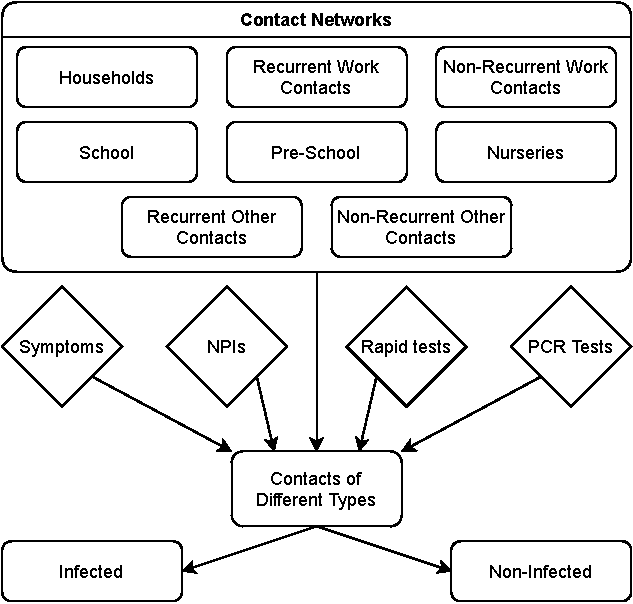
\includegraphics[width=\textwidth]{../figures/model-graph-top-left}
        \caption{{Model description}}
        \label{fig:broad_model_description}
    \end{subfigure}
    \hfill
    \begin{subfigure}[b]{0.425\textwidth}
        \centering
        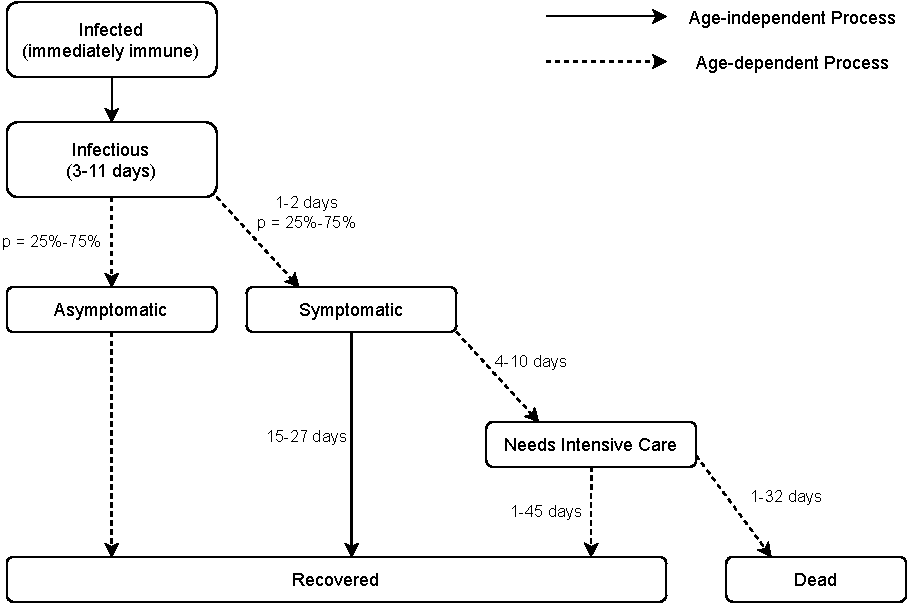
\includegraphics[width=\textwidth]{../figures/model-graph-top-right}
        \vskip4ex


        \caption{Disease progression}
        \label{fig:disease_progression}
    \end{subfigure}
    \vskip3ex
    \begin{subfigure}[b]{0.425\textwidth}
        \centering

        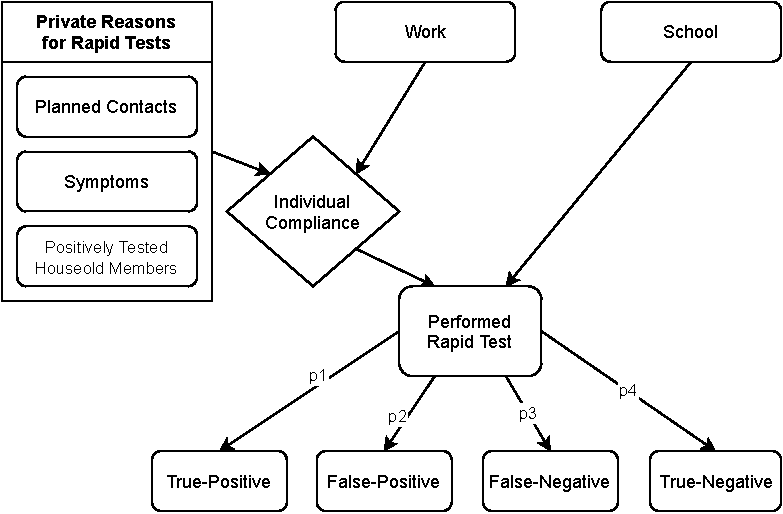
\includegraphics[width=\textwidth]{../figures/model-graph-bottom-left}
        \caption{{Model for antigen tests}}
        \label{fig:antigen_tests}
    \end{subfigure}
    \hfill
    \begin{subfigure}[b]{0.425\textwidth}
        \centering
        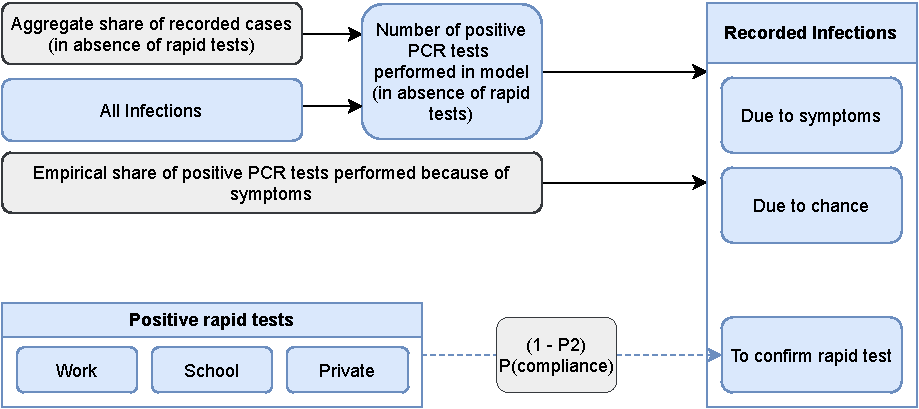
\includegraphics[width=\textwidth]{../figures/model-graph-bottom-right}
        \caption{{Model for undetected cases}}
        \label{fig:model_for_official_cases}
    \end{subfigure}

    \caption{Model description}
    \label{fig:model-description}

    \floatfoot{\noindent Note: ...}
\end{figure}

In our model, susceptibility to contracting the SARS-CoV-2 virus is dependent on age. A
possible infection progresses as shown in Figure~\ref{fig:disease_progression}. We
differentiate between an initial period of infection without being infectious or showing
symptoms, being infectious (presymptomatic or asymptomatic), showing symptoms, requiring
intensive care, and recovery or death as for example also modeled in \cite{Grimm2021}.
The probabilities of transitioning between these states depend on age; their duration is
random within intervals calibrated to medical literature (for a detailed description see
Section~\ref{sec:medical_params}). Conditional on the type of contact, infectiousness is
independent of age \citep{Jones2021}.

The model includes several other features, which are crucial to describe the evolution
of the pandemic in 2020-2021. New virus strains with different profiles regarding
infectiousness can be introduced. Agents may receive a vaccination. With a probability
of 75\% \citep{Hunter2021}, vaccinated agents become immune and they do not transmit the
virus \citep{Petter2021, LevineTiefenbrun2021, Pritchard2021}.\footnote{75\% is
    lower than what is usually reported for after the second dose of the Biontech/Pfizer
    vaccine, which is most commonly used in Germany. We choose it because our model neither
    includes booster shots, nor does it allow vaccinated individuals who became immune to
    transmit the disease\citep{Petter2021, LevineTiefenbrun2021, Pritchard2021}. If
    anything, these assumptions would overstate the effect of vaccines for our study period.
    This would be different if a large fraction of vaccinated individuals had received a
    second dose already.} During the vaccine roll-out, priority may depend on age and
occupation.

We include two types of tests. Polymerase chain reaction (PCR) tests directly reveal
whether an individual is infected or not. PCR tests require some days to be processed and
there are aggregate capacity constraints throughout. In contrast, rapid antigen tests
yield immediate results; after a phase-in period, all tests that are demanded will be
performed. Specificity and sensitivity of these tests is set according to data analyzed
in \cite{Bruemmer2021, Smith2021}; sensitivity depends on the timing of the test relative
to the start of infectiousness. Figure~\ref{fig:antigen_tests} shows our model for rapid
test demand. Schools may require students to be tested regularly. Rapid tests may be
offered by employers for on-site workers. Individuals may demand tests for private
reasons, which include having plans to meet other people\footnote{A positive test will
make them reduce their contacts; this is why tests impact the actual contacts in
Figure~\ref{fig:model-description}.}, showing symptoms of CoViD-19, and because a
household member tested positively for the virus. We endow each agent with an individual
compliance parameter. This parameter determines whether she takes up rapid tests offered
by employers or follows up on private reasons and whether she reduces her contacts if she
tests positive or develops symptoms. The thresholds are higher for tests in a private
setting than for tests at the workplace until mid April and then compliance because of
private reasons becomes higher than compliance at the workplace.

Modelling a population of agents according to actual demographic characteristics means
that we can use a wide array of data to identify and estimate the model's many
parameters.\footnote{See section~\ref{sec:data_and_parameters} of the supplementary
materials for an overview.} We can rely on contact diaries to get pre-pandemic
distributions of contacts for different contact types and their assortativity by age
group. Mobility data is used to model the reductions in work contacts. School and daycare
policies can be incorporated directly from official directives. Aggregate tests,
vaccinations and the prevalence of virus strains can be taken from official records. The
likelihood to receive a test offer or to take up a test offer and the share of
individuals that have ever taken a test or done weekly tests in the last month can be
calibrated from survey data.\comment[id=HM]{Anything else we need to
mention?}\comment[id=K]{I added some more that I think are worth mentioning.} We estimate
the infection probabilities\comment[id=HM]{need to be more precise here, cannot find in
Appendix}\comment[id=K]{I added \ref{subsec:infection_probs}.} that the simulated new
infections predict age- and region-specific time series.\comment[id=K]{We never directly
targeted the federal states if I remember it right. How large was their weight in the
criterion function @Janos?} However, the two sets of time series are not comparable
directly because not all cases will be recorded. We model the fraction of recorded cases
as depicted in Figure~\ref{fig:model_for_official_cases}.\comment[id=HM]{Add a sentence.}

The model is applied to the second and third wave of the CoViD-19 pandemic in Germany,
covering the period mid-September 2020 to the end of May 2021.
Figure~\ref{fig:pandemic_drivers_model_fit} describes the evolution of the pandemic and
of its drivers. The black line in Figure~\ref{fig:aggregated_fit} shows officially
recorded cases; the black line in Figure~\ref{fig:stringency_index} the Oxford Response
Stringency Index \citep{Hale2020}, which tracks the tightness of non-pharmaceutical
interventions. We transform the index so that lower values represent higher levels of
restrictions. A value of zero means all measures incorporated in the index are turned
on. The value 1 represents the situation in mid-September, with restrictions on
gatherings and public events, masking requirements, but open schools and workplaces. In
the seven weeks between mid September and early November, cases increased by a factor of
10. Restrictions were somewhat tightened in mid-October and again in early November. New
infections remained constant throughout November, before rising again in December, which
prompted the most stringent lockdown to this date. Schools and daycare centers were
closed again, so were customer-facing businesses except for grocery and drug stores.
From the peak of the second wave just before Christmas until the trough in mid-February,
newly detected cases decreased by almost three quarters. The third wave in the spring of
2021 is associated with the B.1.1.7 strain, which became dominant in March. See
Figure~\ref{fig:share_b117}. In early March, some NPIs were being relaxed; e.g.,
hairdressers and home improvement stores were allowed to open again to the public. There
were many changes in details of regulations afterwards, but they did not change the
stringency index.

\begin{figure}[!tp]
    \centering

    \begin{subfigure}[b]{0.475\textwidth}
        \centering
        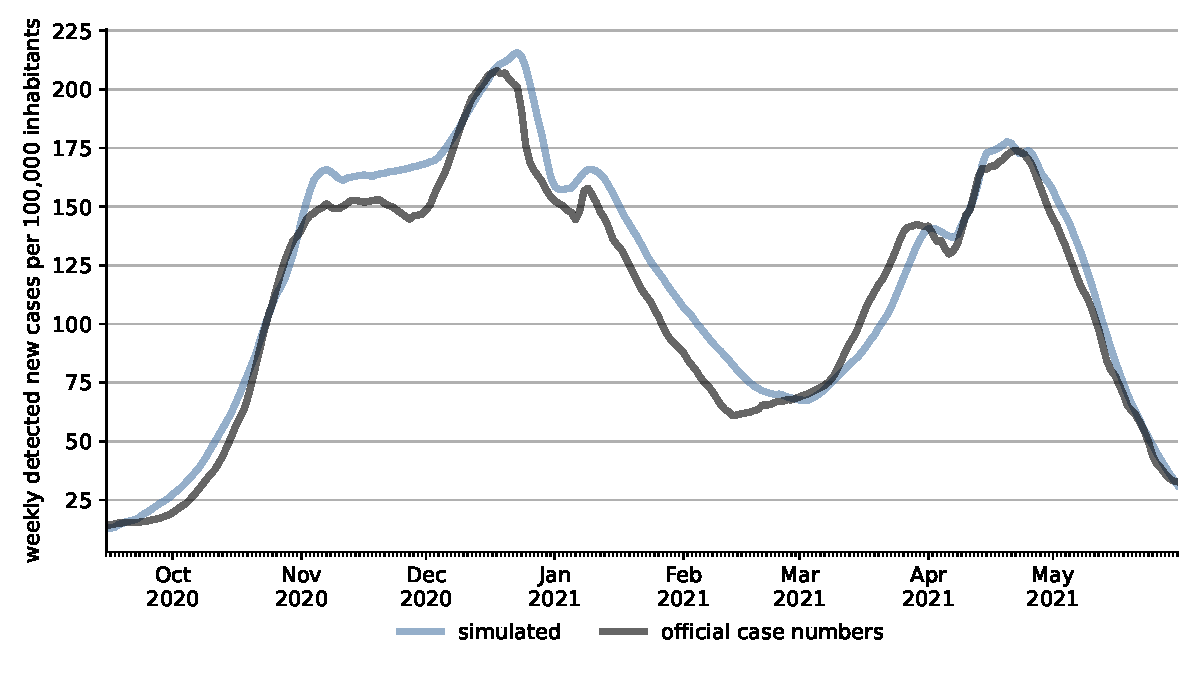
\includegraphics[width=\textwidth]{../figures/results/figures/scenario_comparisons/combined_fit/full_new_known_case}
        \caption{{Recorded cases: Empirical and simulated}}
        \label{fig:aggregated_fit}
    \end{subfigure}
    \hfill
    \begin{subfigure}[b]{0.475\textwidth}
        \centering
        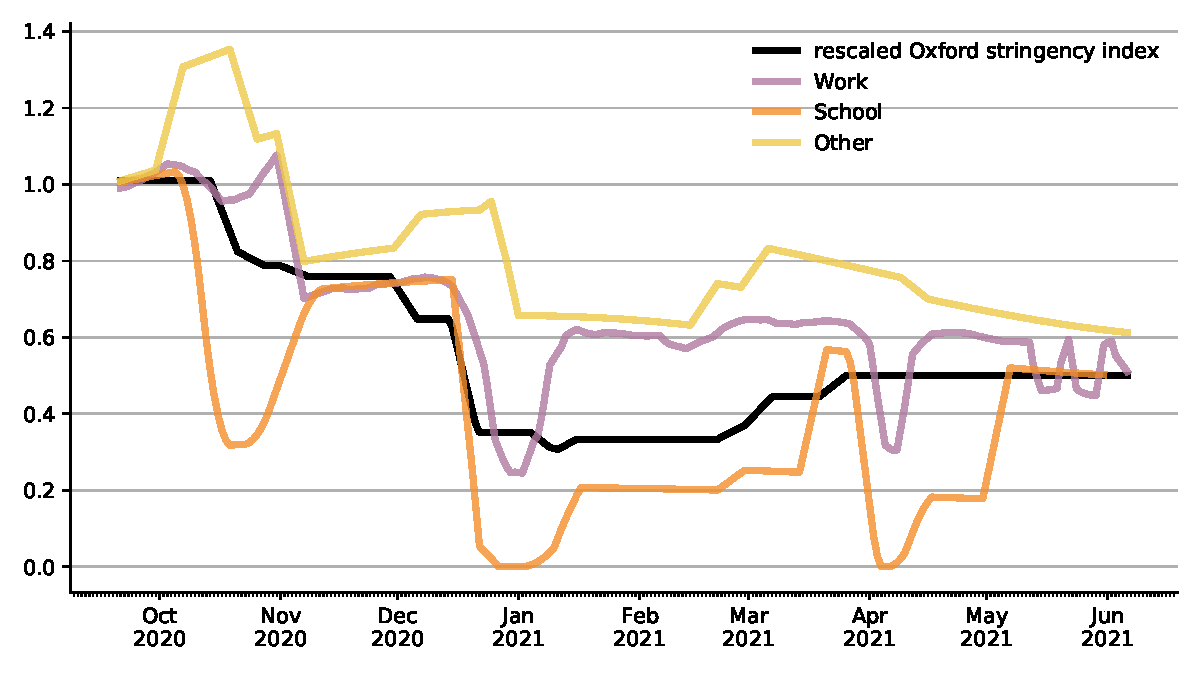
\includegraphics[width=\textwidth]{../figures/results/figures/data/stringency2_with_seasonality}

        \caption{{Stringency of NPIs and infectious contacts}}
        \label{fig:stringency_index}
    \end{subfigure}

    \vskip3ex

    \begin{subfigure}[b]{0.475\textwidth}
        \centering

        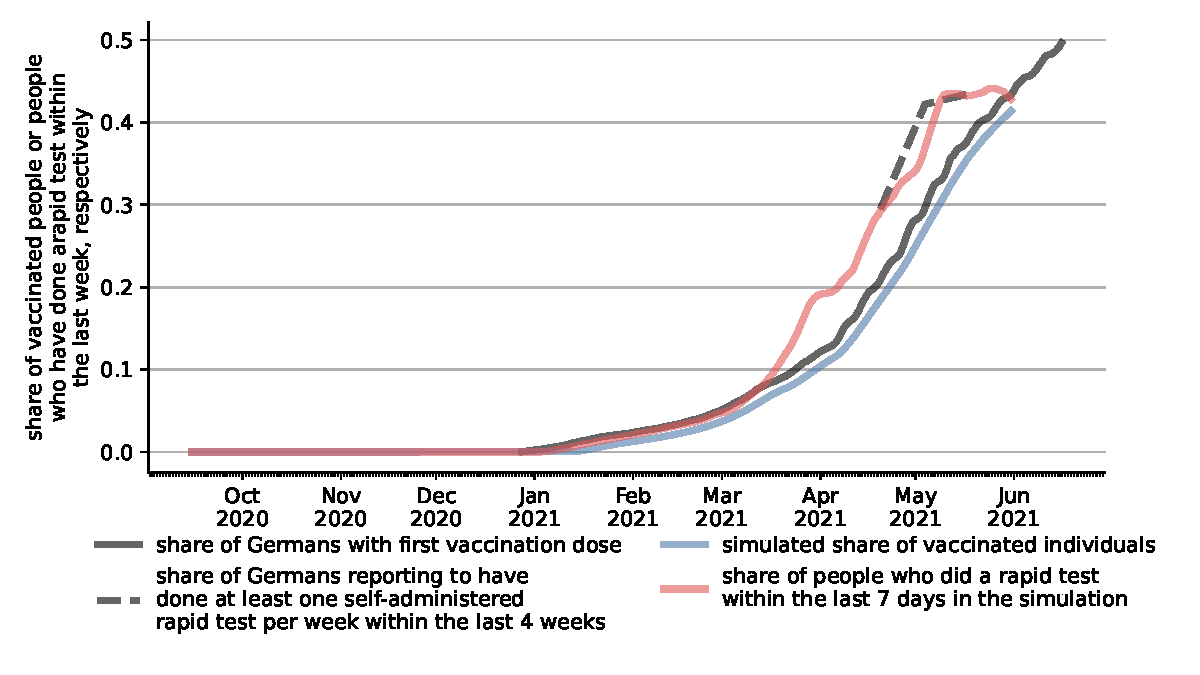
\includegraphics[width=\textwidth]{../figures/results/figures/scenario_comparisons/combined_fit/full_share_rapid_test_in_last_week_and_vaccinated}

        \caption{{Tests and vaccinations}}
        \label{fig:antigen_tests_vaccinations}
    \end{subfigure}
    \hfill
    \begin{subfigure}[b]{0.475\textwidth}
        \centering

        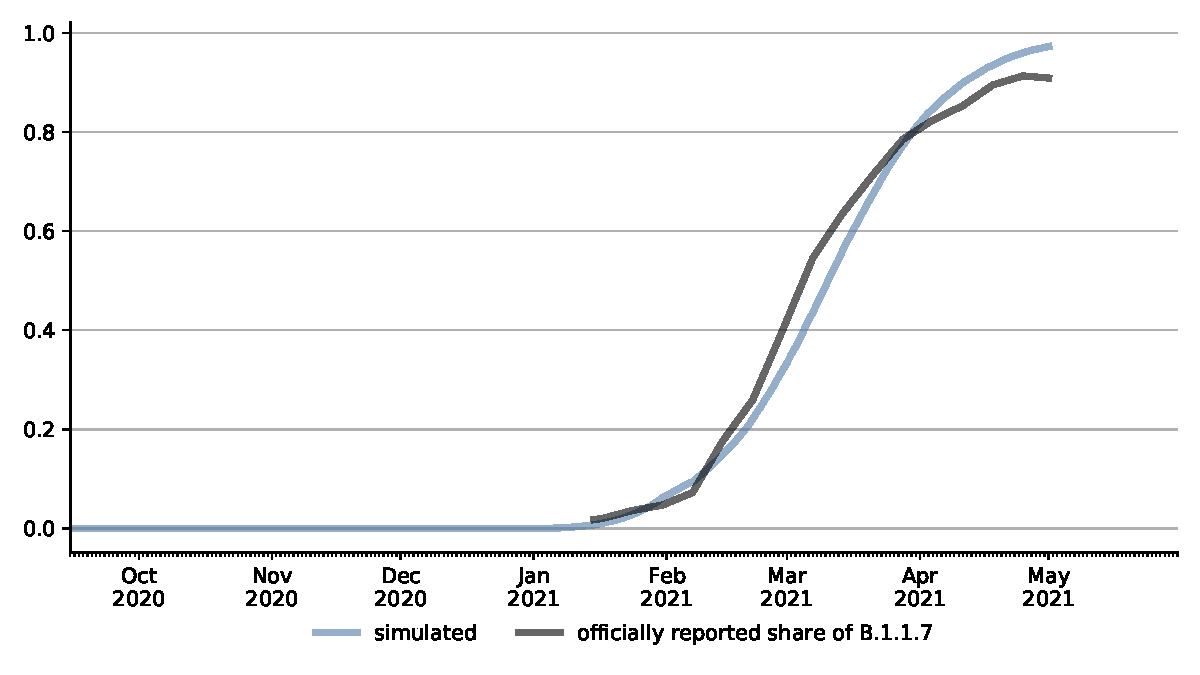
\includegraphics[width=\textwidth]{../figures/results/figures/scenario_comparisons/combined_fit/full_share_b117}

        \caption{Fraction of B.1.1.7 strain}
        \label{fig:share_b117}
    \end{subfigure}

    \caption{Evolution of the pandemic, its drivers, and model fit, September 2020 to May 2021}
    \label{fig:pandemic_drivers_model_fit}

    \floatfoot{\noindent Note: All aggregates; See S.XXX for statistics by age group and
        by geographical region. Also more disaggregated data.

        Sources: ...}

\end{figure}

By this time, the set of policy instruments had become much more diverse. Around the
turn of the year, the first people were vaccinated with a focus on older age groups and
medical personnel (Figure~\ref{fig:antigen_tests_vaccinations}. By the end of May, just
over 40\% had received at least one dose of a vaccine. Around the same time, rapid tests
started to replace regular PCR tests for staff in many medical and nursing facilities.
These had to be administered by medical doctors or in pharmacies. At-home tests approved
by authorities became available in mid-March, rapid test centers were opened and one
test per person and week was made available free of charge. Depending on the state,
customers were only allowed to enter certain stores with a recent negative rapid test
result. These developments are characteristic of many countries: The initial focus on
NPIs to slow the spread of the disease has been accompanied by vaccines and a growing
acceptance and use of rapid tests. At broadly similar points in time, novel strains of
the virus have started to pose additional challenges.

We draw simulated samples of agents from the distribution of recorded infections in
September 2020 and use the model to predict recorded infection rates until the end of
May 2021. See Supplementary Materials~\ref{sec:data_and_parameters} and \ref{sec:model}
for detailed descriptions of the data and the model, respectively. The blue line in
Figure~\ref{fig:aggregated_fit} shows our model's predictions are very close to
officially recorded cases in the aggregate. This is also true for infections by age and
geographical region, which are shown in the supplementary materials
(Figures~\ref{fig:age_group_fit} and \ref{fig:state_fit}, respectively).

The effects of various mechanisms can be disentangled due to the distinct temporal
variation in the drivers of the pandemic. Next to the stringency index, the three lines
in Figure~\ref{fig:stringency_index} summarize how contact reductions, increased hygiene
regulations, and seasonality evolved since early September for each of the three broad
contact networks. For example, a value of 0.75 for the work multiplier means that if the
environment was the same as in September (levels of infection rates, no rapid tests or
vaccinations, only the wildtype virus present), infections at the workplace would be
reduced by 25\%. The lines show the product of the effect of contact reductions,
increased hygiene regulations, and seasonality. See Appendix~\comment[id=HM]{Reference}
for separate plots of the three factors. Two aspects are particularly interesting.
First, all lines broadly follow the stringency index and they would do so even more if
we left out seasonality and school vacations (roughly the last two weeks of October, two
weeks each around Christmas and Easter, and some days in late May). Second, the most
stringent regulations are associated with the period of strong decreases in new
infections between late December 2020 and mid-February 2021. The reversal of the trend
is associated with he spread of the B.1.1.7 variant. The steep drop in recorded cases
during May 2021 is associated with at least weekly rapid tests to around 42~percent of
the population, a vaccination rate that rose from 28\% to 43\%, and mostly seasonality
impacting a fall in the relative infectiousness of contacts outside of work and school.

In order to better understand the contributios  of rapid tests, vaccinations, and of
seasonality on the evolution of infections in 2021,
Figure~\ref{fig:2021_scenarios_broad} considers various scenarios. NPIs are always the
same as in the baseline scenario. Figure~\ref{fig:2021_scenarios_recorded} shows the
model fit (the blue line, same as in Figure~\ref{fig:aggregated_fit}), a scenario
without any of the three factors (red line), and three scenarios turning these factors
off one by one. Figure~\ref{fig:2021_scenarios_newly_infected} does the same for total
infections in the model. Figure~\ref{fig:2021_scenarios_decomposition} employs Shapley
values to decompose the difference in total infections between the scenario without any
of the three factors and our main specification.

\begin{figure}[!tp]
    \centering

    \begin{subfigure}[b]{0.475\textwidth}
        \centering
        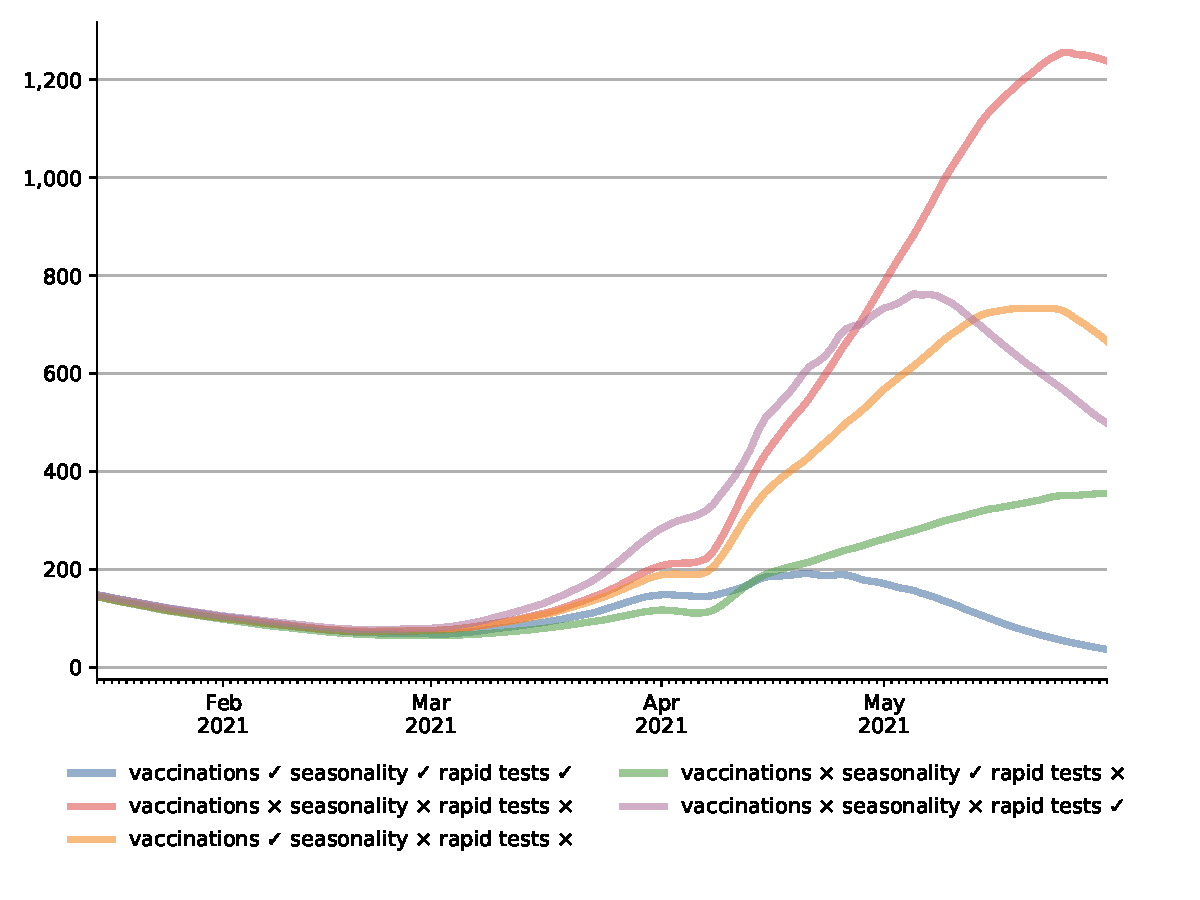
\includegraphics[width=\textwidth]{../figures/results/figures/scenario_comparisons/effect_of_channels_on_pessimistic_scenario/full_new_known_case}
        \caption{{Recorded cases: 2021 scenarios}}
        \label{fig:2021_scenarios_recorded}
    \end{subfigure}
    \hfill
    \begin{subfigure}[b]{0.475\textwidth}
        \centering
        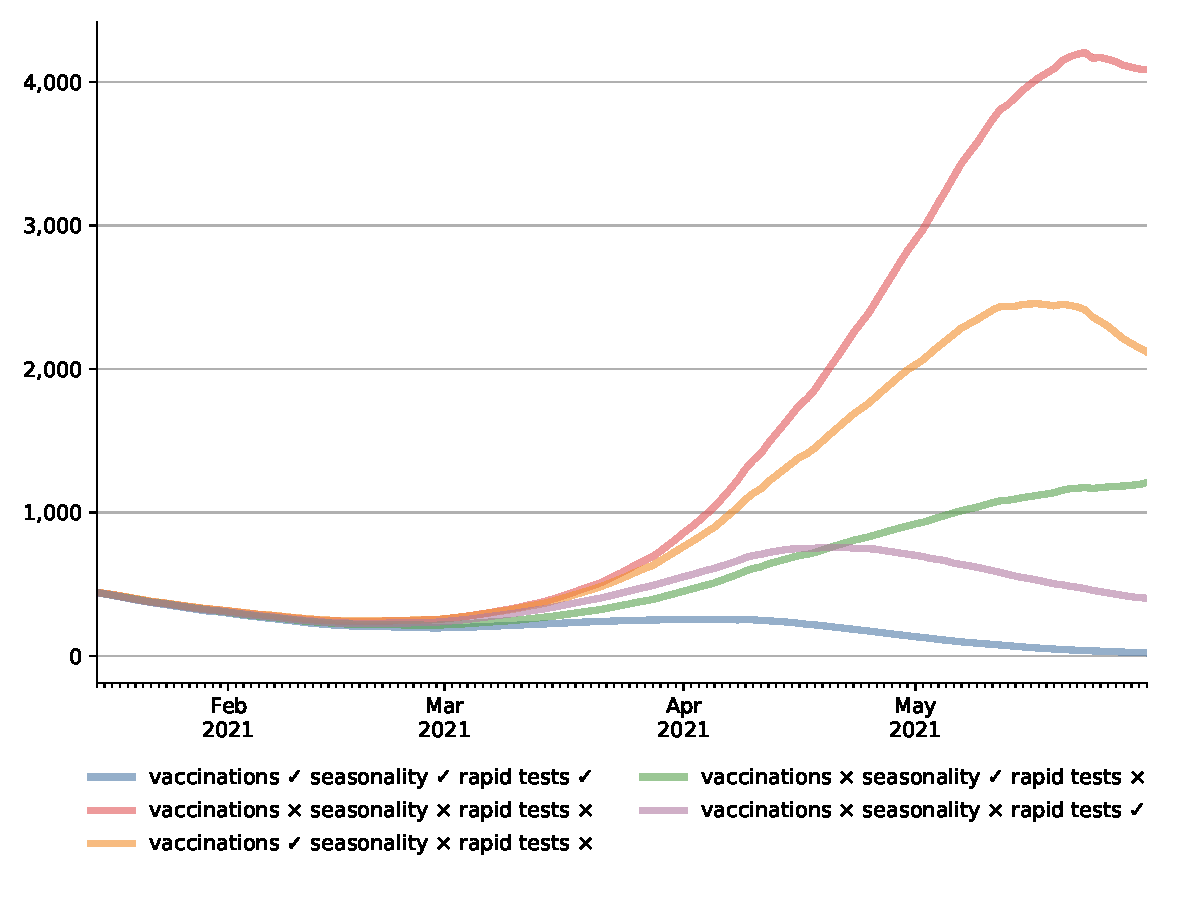
\includegraphics[width=\textwidth]{../figures/results/figures/scenario_comparisons/effect_of_channels_on_pessimistic_scenario/full_newly_infected}
        \caption{{Total cases: 2021 scenarios}}
        \label{fig:2021_scenarios_newly_infected}
    \end{subfigure}

    \begin{subfigure}[b]{0.475\textwidth}
        \centering
        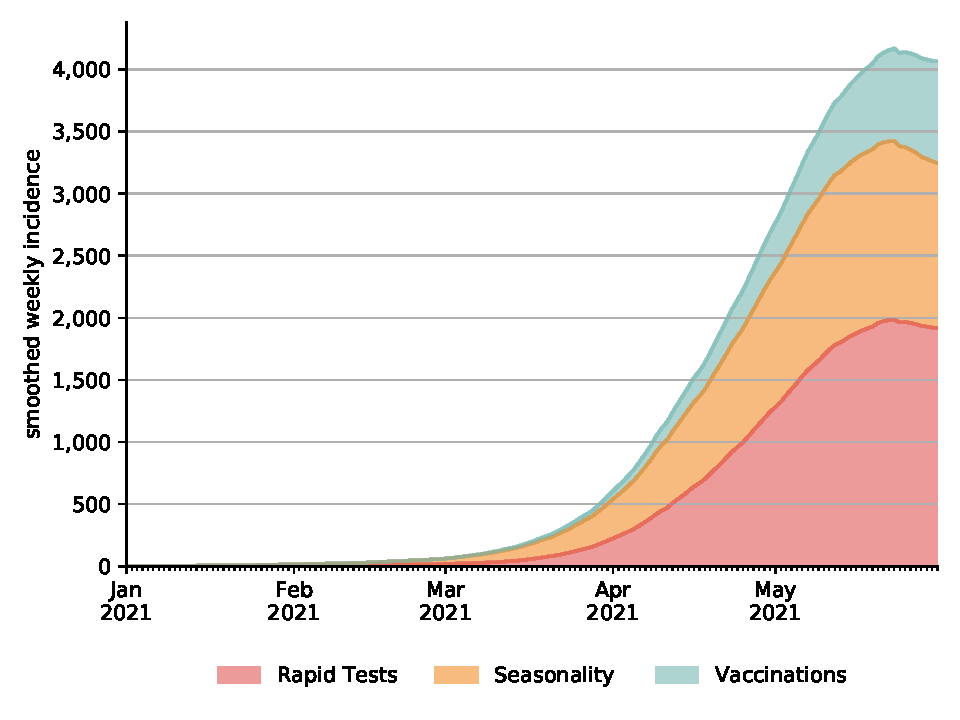
\includegraphics[width=\textwidth]{../figures/results/figures/full_decomposition_channels_area}
        % 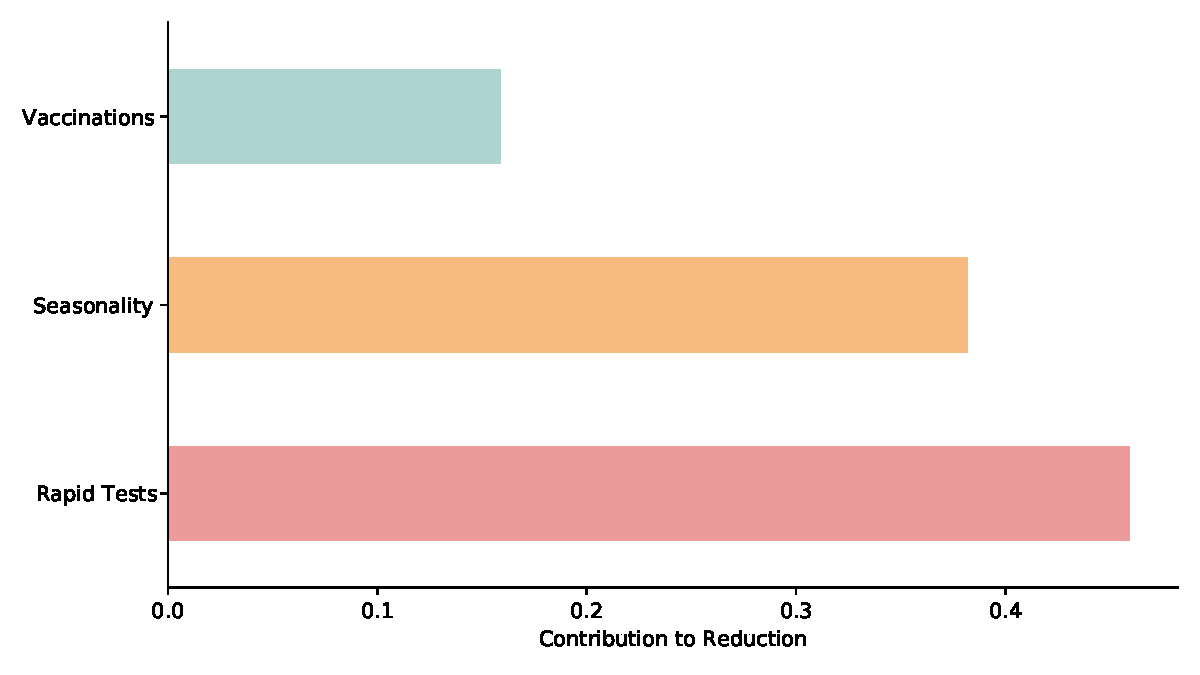
\includegraphics[width=\textwidth]{../figures/results/figures/full_decomposition_channels_bar}
        \caption{Decomposition of the difference between the scenario without any of the
            three factors and the main scenario in
            Figure~\ref{fig:2021_scenarios_newly_infected}.}
        \label{fig:2021_scenarios_decomposition}
    \end{subfigure}
    \hfill
    \begin{subfigure}[b]{0.475\textwidth}
        \centering
        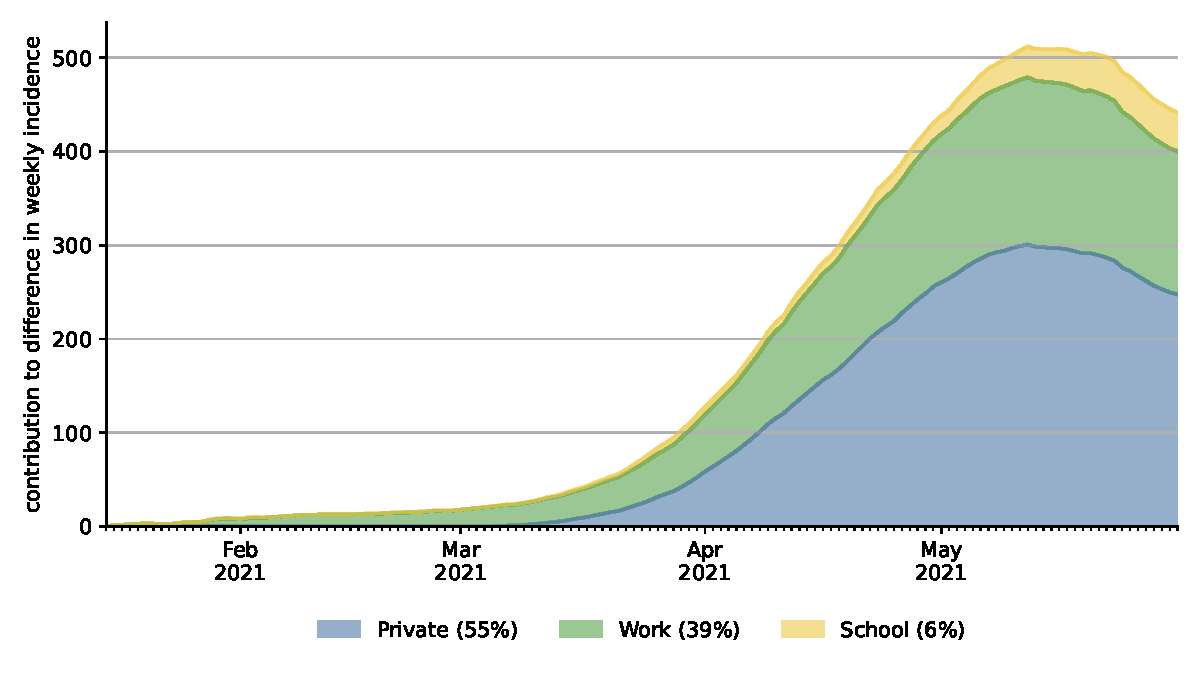
\includegraphics[width=\textwidth]{../figures/results/figures/full_decomposition_rapid_tests_area}
        % 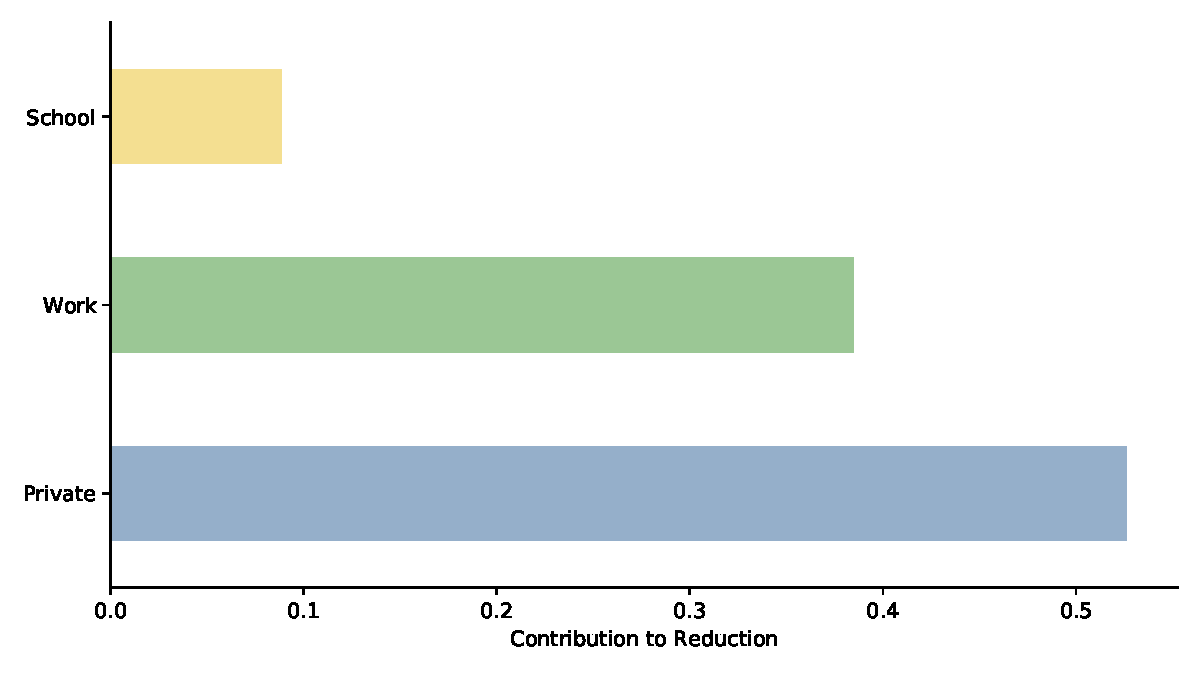
\includegraphics[width=\textwidth]{../figures/results/figures/full_decomposition_rapid_tests_bar}
        \caption{Decomposition of the difference between the scenario without rapid
            tests and the main scenario in Figure~\ref{fig:2021_scenarios_newly_infected}.}
        \label{fig:2021_scenarios_decomposition_tests}
    \end{subfigure}

    \caption{The effect of different interventions on recorded and actual infections}
    \label{fig:2021_scenarios_broad}

    \floatfoot{\noindent Note: All aggregates; See S.XXX for statistics by age group and
        by geographical region.

        The decomposition is based on Shapley values where the individual contribution
        of a channel is its average contribution over different sizes of coalitions
        (combinations with other channels). The individual contribution to a coalition
        is the difference between the effect size of the coalition with the particular
        channel and without.}
\end{figure}

Until mid-March, there is no visible difference between the different scenarios.
Seasonality hardly changes, and only few vaccinations or rapid tests were administered.
Even thereafter, the effect of the vaccination campaign is surprisingly small at first
sight. Whether considering recorded or total infections with only one channel active,
the final level is always the highest in case of the vaccination campaign (orange
lines). The Shapley value decomposition shows that vaccinations contribute about 15\% to
the cumulative difference between scenarios. Reasons for this are the slow start---it
took until March~24th until 10\% of the population had received their first vaccination,
the 20\% mark was reached on April 19th---and the focus on older individuals. These
groups contribute less to the spread of the disease than others due to a lower number of
contacts, see Supplementary Material~\ref{subsec:contacts_by_age}. It is important to
note that the initial focus of the campaign was to prevent deaths and severe disease;
the case fatality was rate considerably lower during the third wave when compared to the
second (4.4\% between October and February and 1.4\% between March and June). It is
important to note that by the end of our study period, when first-dose vaccination rates
reached around 40\% of the population, the numbers of new cases would have started to
decline.

Seasonality has a large effect in slowing the spread of SARS-CoV-2. By May 31, both
observed and recorded cases would be reduced by a factor of four if only seasonality
mattered. However, in this period, cases would have kept on rising throughout, just at a
much lower pace. Nevertheless, we estimate it to be a quantitatively important factor
determining the evolution of the pandemic, explaining most of the early changes and
almost 40\% of the cumulative difference by the end of May.

The largest effect---almost one half when considering the decompositions---comes from
rapid testing. Here, it is crucial to differentiate between recorded cases and actual
cases. Additional testing means that infections become known, which would otherwise
remain undetected. Figure~\ref{fig:2021_scenarios_recorded} shows that this means that
until late April, recorded cases are higher than in the scenario where none of the three
mechanisms is turned on. Compared to the scenario with vaccinations only, this point is
reached around mid-May and it would be June for the comparison with the seasonality-only
scenario. The effect on total cases, however, is visible immediately. Despite the fact
that only a small fraction of the population performed weekly rapid tests in
March\footnote{X\% in the model; 27\% of respondents to the COSMO study reported in
    early March that they \textit{ever} did a rapid test)}\comment[id=HM]{Put in}, new
infections on April 1 would be reduced by 53\% relative to the scenario without
vaccinations, rapid tests, or seasonality.

So why is rapid testing so effective? In order to shed more light on this question,
Figure~\ref{fig:2021_scenarios_decomposition_tests} decomposes the difference in the
scenario without rapid tests only (purple line in
Figure~\ref{fig:2021_scenarios_newly_infected}) and the main specification into the
three channels for rapid tests. Tests for pupils have the smallest effect, which is
largely explained by the relatively small number of students (XXM pupils vs. YYM
workers)\comment[id=HM]{fill in} and the fact that schools did not operate at full
capacity during our period of study. Almost 40\% come from tests at the workplace.
Despite the fact that we phase rapid tests for private reasons are phased in only late,
they make up for more than half of the total effect.

\comment[id=HM]{How many tests are actually performed along each of the three dimensions? Could this be a quantity story rather than the directed testing story I am making up here as wishful thinking?}

The reason lies in the fact that a substantial share of these tests is driven by an
elevated probability to carry the virus, i.e., showing symptoms of CoViD-19 or following
up on a positive test of a household member. The latter is essentially a form of contact
tracing, which has been shown to be very effective.\comment[id=HM]{cite Priesemann
paper, others?} This is also the reason for why the number of tests performed fall at
the very end of our study period. Falling infection rates mean that there are fewer
events triggering private test demand.
\comment[id=HM]{Positive rates along the three channels might be nice here, if previous comment is not a quant story}
\comment[id=HM]{I think there is a story in here about risk conditional on past exposure vs. prospective risk in gatherings, but it is too late to work through it. We might just want to calculate the probabilities.}

Two of the most contentious NPIs concern schools and mandates to work from home. In many
countries, schools switched to remote instruction during the first wave, so did Germany.
After the summer break, they were operating at full capacity with increased hygiene
measures, before being closed again from mid-December on. Some states started opening
them gradually in late February, but usual operaton was not back until the beginning of
June. Figure~\ref{fig:school_scenarios} shows the effects of different policies regarding school starting at Easter, a point where rapid tests had become widely available. 

In light of the large negative effects school closures have on children and
parents\comment[id=HM]{need to cite a couple of poor learning outcomes / mental health
papers. There must be well-published ones}---and in particular on those with low
socio-economic status---the results in

Effects:
\begin{itemize}
    \item Schools were essentially closed
    \item What are the different $R_t$-values? In no-test scenario and $R_t>1$, might be
          worth chopping off 0.05 or whatever that might be?
    \item With tests it is really hard to make a case for that
\end{itemize}

Alternative:
\begin{itemize}
    \item Germany quite lenient on home office relative to other countries (employer had
          to allow)
    \item Testing: Rapid tests are cheap (less than 1\euro), just a nuisance.
\end{itemize}

Results
\begin{itemize}
    \item Advantage of testing in both cases: Recurrent. Small cost relative to other
          stuff. Certain publicness.
    \item Mandatory tests: Screening effect for hard-to-reach populations (do not
          consider in this paper, also due to poor data in DE)
\end{itemize}


\begin{figure}[!tp]
    \centering

    \begin{subfigure}[b]{0.475\textwidth}
        \centering
        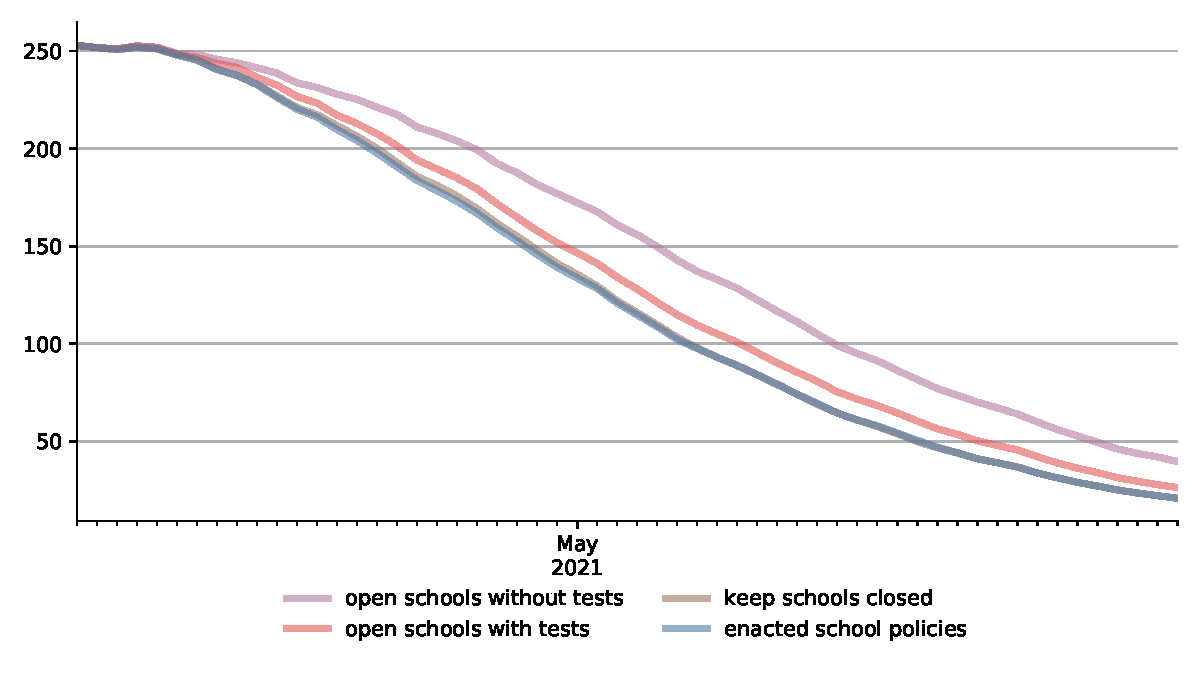
\includegraphics[width=0.9 \textwidth]{../figures/results/figures/scenario_comparisons/school_scenarios/full_newly_infected}
        \caption{{Effects of different schooling scenarios}}
        \label{fig:school_scenarios}
    \end{subfigure}
    \hfill
    \begin{subfigure}[b]{0.475\textwidth}
        \centering
        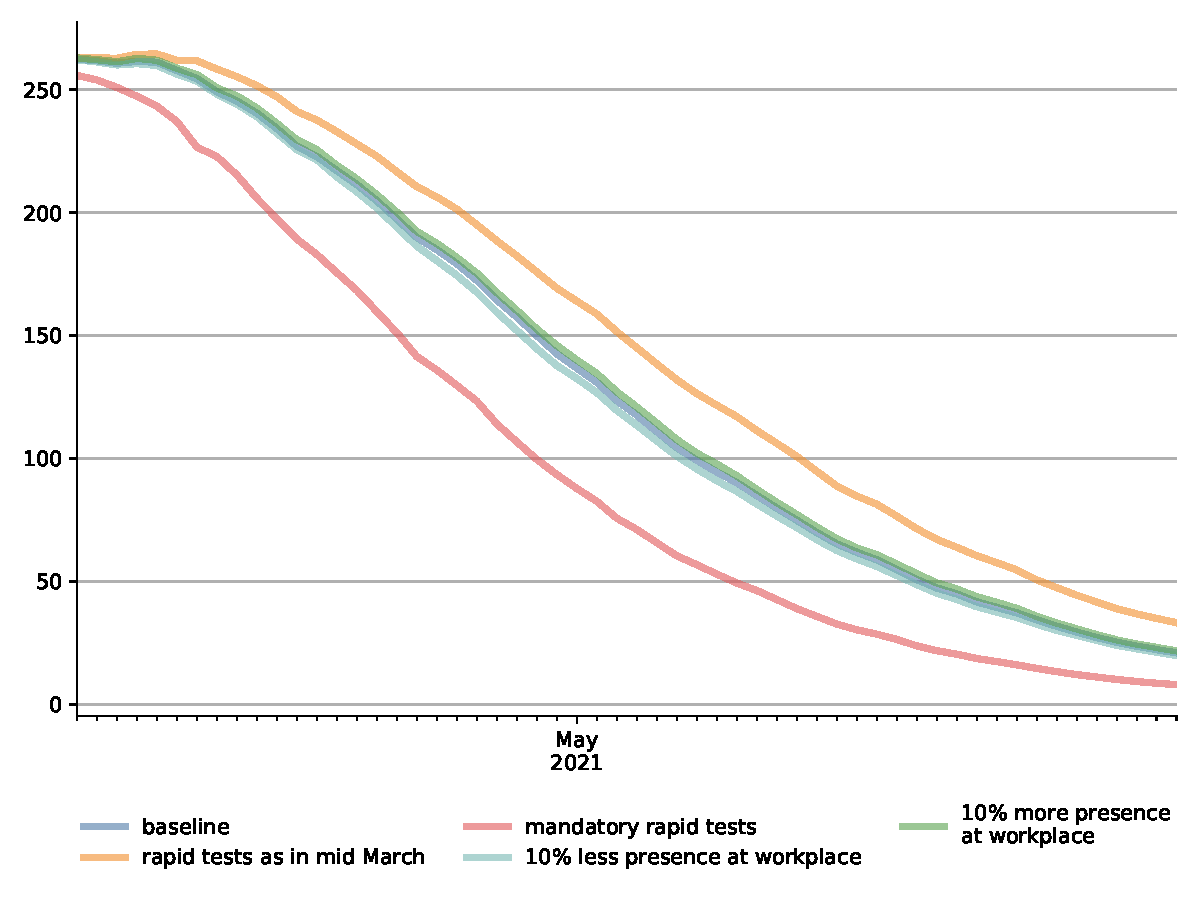
\includegraphics[width=0.9 \textwidth]{../figures/results/figures/scenario_comparisons/new_work_scenarios/full_newly_infected}
        \caption{{Effects of different work scenarios}}
        \label{fig:workplace_scenarios}
    \end{subfigure}
    \vskip3ex

    \caption{Effects of different scenarios for policies regarding schools and workplaces.}
    \label{fig:school_workplace_scenarios}

    \floatfoot{\noindent Note: Interventions start at Easter because there were no
        capacity constraints for rapid tests afterwards.}

\end{figure}


\phantomsection % Needed for the bibliography bookmark to point to the correct page

\begin{refcontext}[sorting=none]  % Sort BIBLIOGRAPHY by appearance.
    \printbibliography[heading=bibintoc]
\end{refcontext}

\clearpage
\setcounter{page}{1}
\begin{appendices}

    \begin{refsection}
        \begin{center}
            {
                \Large
                Supplementary Material for\\[2ex]

                \textbf{\papertitle}
            }
            \vskip4ex
            {
                \large
                Janoś Gabler,

                Tobias Raabe,

                Klara Röhrl,

                Hans-Martin von Gaudecker

            }
        \end{center}

        \tableofcontents
        \clearpage

        \section{Materials and Methods}
\label{sec:materials_and_methods}

The model is described by a large number of parameters that govern the number of contacts
a person has, the reduction in contacts due to NPIs, the demand for rapid tests and PCR
tests, the likelihood of becoming infected on each contact, the likelihood of developing
light or strong symptoms or even dying from the disease as well as the duration each
stage of the disease takes.

\subsection{Course of the Disease}
\label{sub:course_of_disease}

The following medical parameters describing the progression of the disease are taken from systematic reviews (e.g. \citet{He2020}). After an infection occurs, the disease progresses in the way depicted in Figure~\ref{fig:course_of_disease}.

\begin{figure}[!tp]
    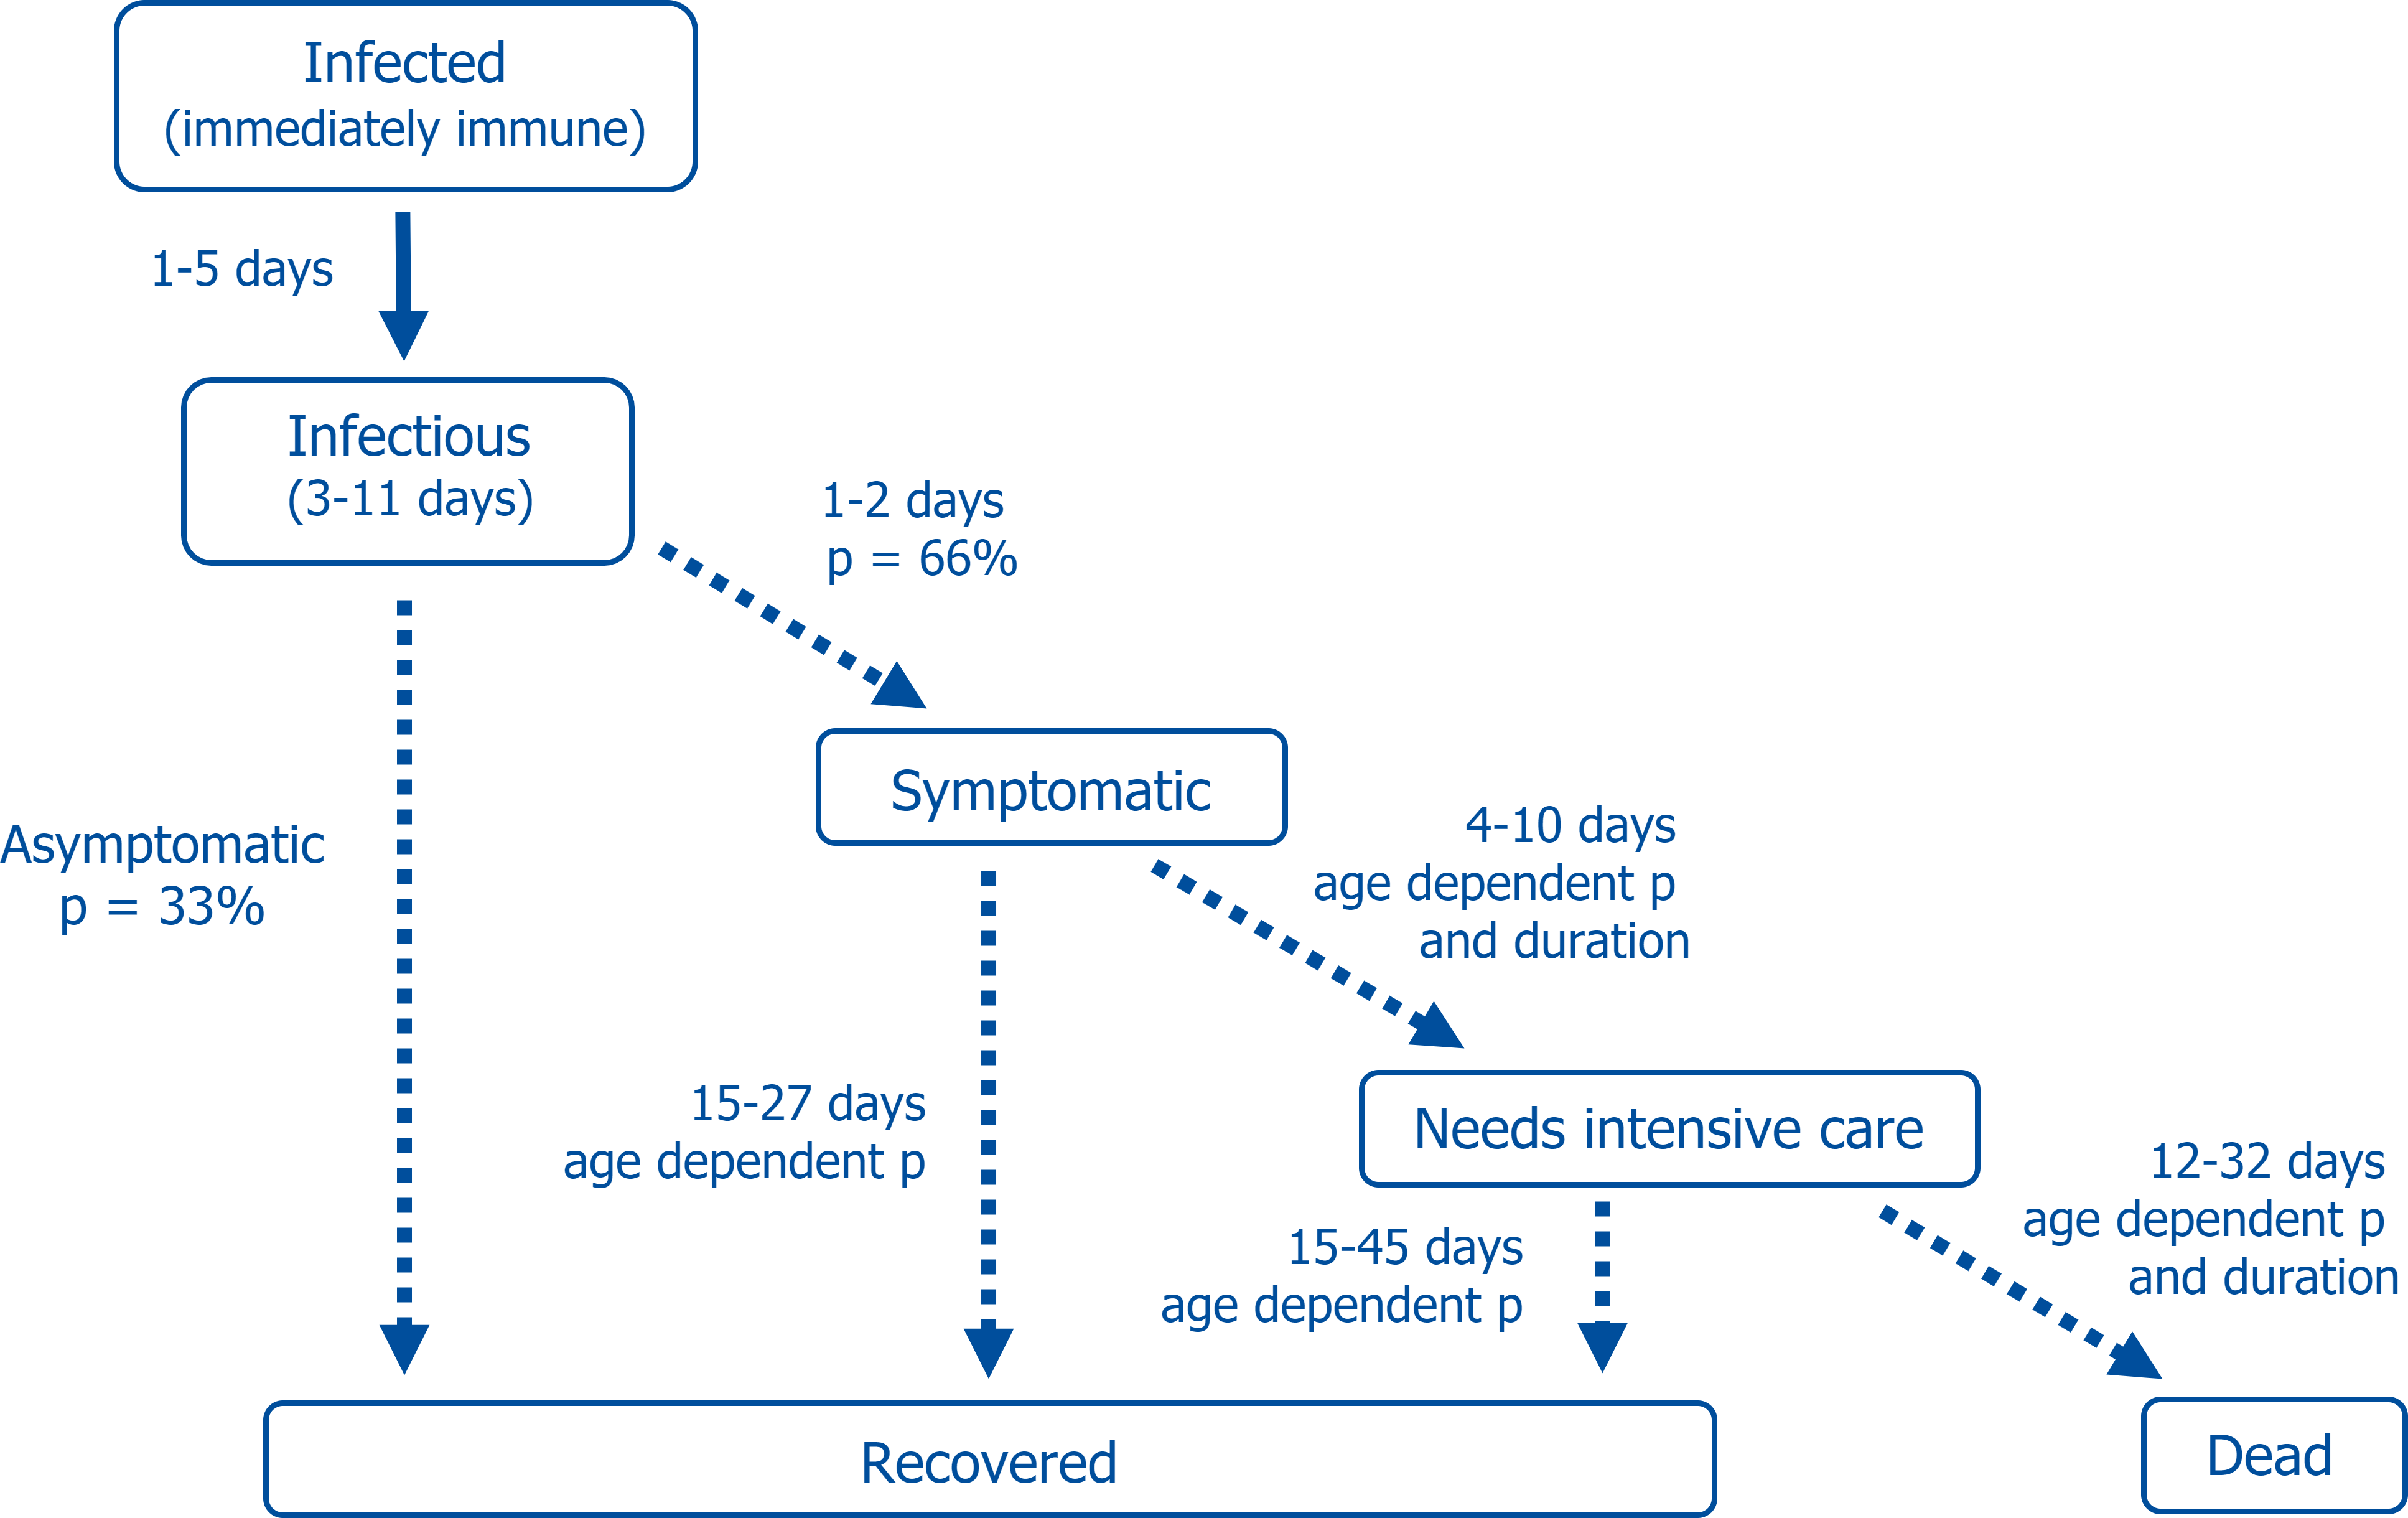
\includegraphics[width=\textwidth]{../figures/disease_progression.png}
    \caption{Course of Disease in the model}
    \label{fig:course_of_disease}
\end{figure}

First, infected individuals will become infectious after one to five days. About one third of people stays asymptomatic. The rest develops symptoms about one to two days after they become infectious. Modeling asymptomatic and pre-symptomatic cases is important because those people do not reduce their contacts or demand a test and can potentially infect many other people \citep{Donsimoni2020}.

A small share of symptomatic people will develop strong symptoms that require intensive care. The exact share and time span is age-dependent. An age-dependent share of intensive care unit (ICU) patients will die after spending up to 32 days in intensive care. Moreover, if the ICU capacity was reached, all patients who require intensive care but do not receive it die.

It would be easy to make the course of disease even more fine-grained. For example, we could model people who require hospitalization but not intensive care. So far we opted against that because only the ICU capacity might become a bottleneck in Germany.

We allow the progression of the disease to be stochastic in two ways: Firstly, state changes only occur with a certain probability (e.g. only a fraction of infected individuals develops symptoms). Secondly, the number of periods for which an individual remains in a state is drawn randomly. The parameters that govern these processes are taken from the literature. They can vary with the age of an individual.

Detailed information on the calibration of the disease parameters is available as part of our \href{https://sid-dev.readthedocs.io/en/latest/reference_guides/epi_params.html}{online documentation}.


\subsection{The Synthetic Population}
\label{subsec:synthetic_population}

We build a synthetic population based on the German microcensus \citep{FDSAeDBUDL2018}.
We only use private households, i.e. exclude living arrangements such as nursing homes as
non-private households vary widely in size and it is very difficult to know which
contacts take place in such living arrangements.

We sample households to build our synthetic population of over one million households
keeping for each of the 2.3 million individuals their age, gender, occupation and whether
they work on Saturdays and Sundays. For each household we draw its county and set the
corresponding federal state.% we draw the county because county is not part of the campus file

We randomly assign 35\% of children below three to attend a nursery \citep{Destatis2020}.
For children between three and six years old, we assume all go to preschool (officially
92.5\% according to \cite{Destatis2020}).
% nurseries and preschools
Children that attend a nursery meet in groups of four \citep{BertelsmannStiftung2019}
plus one adult care taker every weekday when there are no school vacations. Preschool
children meet in groups of nine \citep{BertelsmannStiftung2019} with two adult care
takers. These groups are mixed with respect to age but all belong to the same state and
mostly to the same county.

% school
Every child that goes to school is part of a school class. Each school class meets
three times per weekday, each time with a different set of two teachers, unless
there are vacations or policies that suspend schools.\footnote{We
implement vacations on the federal state level.} Each class consists of approximately 23
students \citep{OECD2013}. All students in a class are of the same age
and live in the same state and mostly also in the same county. In addition, each
child gets assigned a value that captures his or her need to attend nursery, preschool or
school. This allows us to capture various degrees of emergency care that can be granted
while educational facilities are closed or are on some kind of rotating schedule.

% workers
Workers are assigned to a daily meeting work group. The group sizes vary to match the
number of daily repeating work contacts reported by working individuals in
\cite{Mossong2008}. These groups only consist of workers that work in the same county.
For a distribution of the number of daily recurring work contacts see
Figure~\ref{fig:n_contacts_work_daily_recurrent}. To match the number of weekly work groups
we match each worker with up to 14 other workers into pairs to match the number of
reported weekly work contacts shown in Figure~\ref{fig:n_contacts_work_weekly_recurrent}.
Each pair is assigned a weekday on which they always meet in the absence of work
policies. 80\% of these contacts are individuals from the same county.
% work contact priority
In the same way children have an educational priority determining if they are entitled to
emergency care workers are assigned a work contact priority that captures how necessary
their work is and to which degree they can work from home. This means that it's always
the same individuals that continue to have work contacts when work from home mandates of
a certain strictness are in place.

% other recurring contacts
In addition to creating groups for educational facilities and work we also have other
recurring contacts to represent things like groups of friends or sports teams that
practice regularly together. Both daily and weekly groups are created analogously to the
work groups but matching the numbers in Figure~\ref{fig:n_contacts_other_daily_recurrent}
and Figure~\ref{fig:n_contacts_other_weekly_recurrent}. In addition, since leisure
contacts are highly assortative by age all individuals that have a daily leisure contact
are matched with a person not only from the same county but also from the same age group.

% individual responses
The individuals in our population can react to events such as developing symptoms that
are typical of CoViD-19, a positive PCR test or a positive rapid test by reducing their
contacts. To determine who would reduce their contacts in such a situation or demand a
rapid test we introduce a quarantine compliance parameter. Similarly, we introduce a
rapid test compliance parameter that determines in which order individuals start
demanding rapid tests when rapid tests become increasingly available. This makes sure
that when for example only 10\% of workers get tested, it's the same workers that have
access to tests every week.

% vaccination rank
Lastly, for the distribution of vaccinations every individual is assigned a vaccination
group and a vaccination rank from that group that creates a complete vaccination queue
over the population including a share that refuses to be vaccinated ($\xi$) which we
calibrate to  15\% \citep{RKI2021c}. The vaccination groups are created to match the
recommendations by the Ständige Impfkommission \citep{VygenBonnet2020}.\footnote{We cover
that teachers were prioritized more than recommended by the commission.} To cover that
the Pfizer-BioNTech vaccine was later approved for younger age groups we put adolescents
and children into two groups that follow after the general population. These groups do
not become eligible within our simulation frame until June. The way vaccinations are
rolled out in our model is shown in Figure~\ref{fig:vaccinations_by_age_group}.

\begin{figure}[ht]   % vaccinations by age group
  \centering
  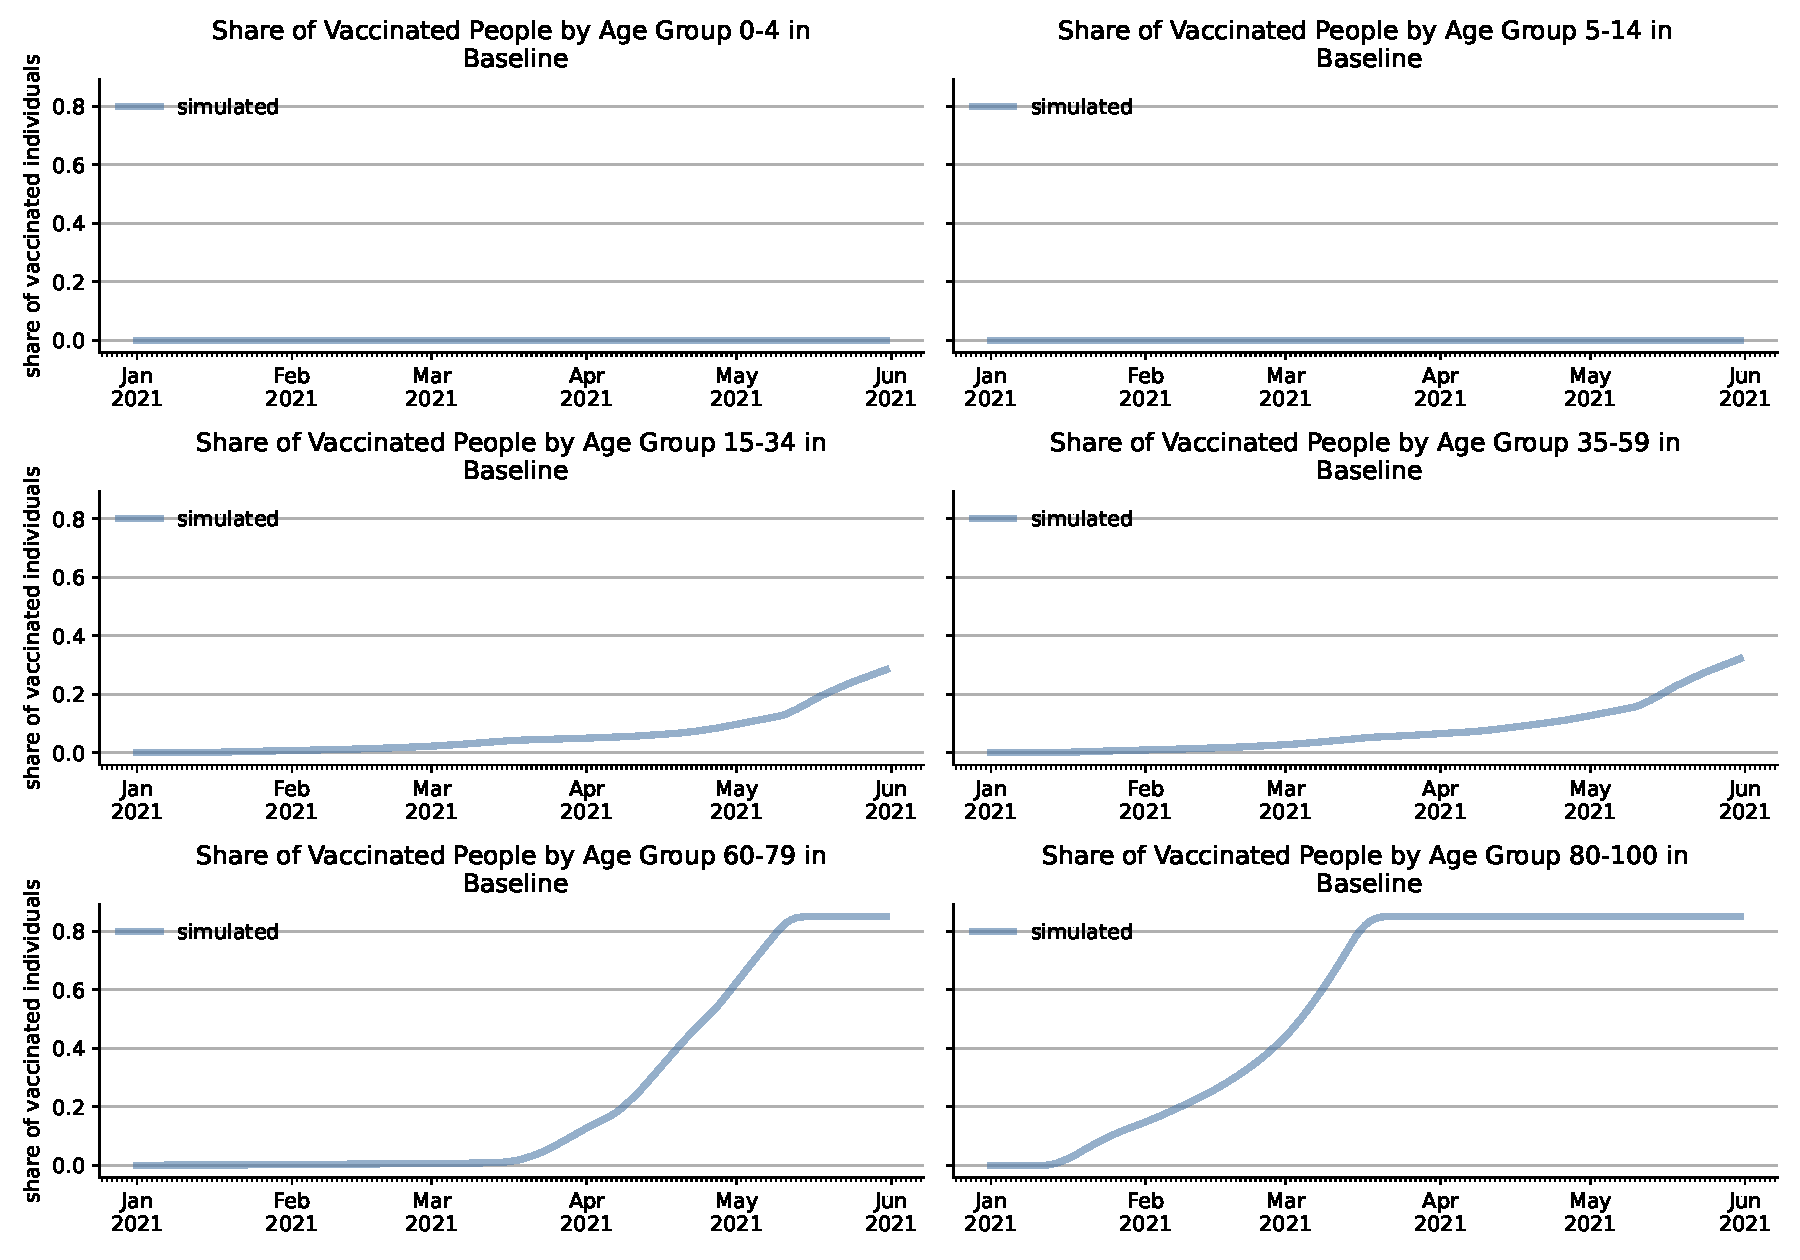
\includegraphics[width=\textwidth]{figures/results/figures/vaccinations/spring_baseline}
  \caption{Vaccination Rates by Age Group}
  \floatfoot{\noindent \textit{Note:} An individual's vaccination priority depends on her
  work contact priority, her age group and a random component to capture
  preconditions like diabetes. 15\% of the population refuse to be vaccinated ($\xi$).
  Adolescents would be vaccinated after the general population and children last. The
  figure clearly shows that the first vaccinations go to some workers with very high work
  contact priority and to the 80 to 100 age group followed by the 60 to 79 year olds.
  Both groups are saturated with vaccinations by mid March and start of May respectively.
  By June a third of the younger adults have received the vaccination but these groups
  still remain far from herd immunity thresholds.}
  \label{fig:vaccinations_by_age_group}
\end{figure}

\FloatBarrier


\subsection{Modeling Numbers of Contacts}
\label{sec:number_of_contacts}

Consider a hypothetical population of 1,000 individuals in which 50 were infected with a
novel infectious disease. From this alone, it is impossible to say whether only
those 50 people had contact with an infectious person and the disease has an infection
probability of 1 per contact or whether everyone met an infectious person but the
disease has an infection probability of only 5 percent per contact. SEIR models do not
distinguish contact frequency from the infectiousness of each contact and
combine the two in one parameter that is not invariant to social distancing policies.

To model social distancing policies, we need to disentangle the effects of the number of
contacts of each individual and the effect of policy-invariant infection probabilities
specific to each contact type. Since not all contacts are equally infectious, we
distinguish different contact types.

The number and type of contacts in our model can be easily extended. Each type of
contacts is described by a function that maps individual characteristics, health states
and the date into a number of planned contacts for each individual. This allows to model
a wide range of contact types.

In our empirical application we distinguish the following  contact types that
are depicted in Figure~\ref{fig:model_contacts_infections} and can be further grouped
in the categories household, work, education and others.

types of contacts:

\begin{itemize}
    \item Households: Each household member meets all other household members every day.
    % Household sizes and structures are calibrated to be representative for Germany.


    \item Recurrent work contacts, capturing contacts with coworkers, repeating
          clients and superiors. Some of these recurrent contacts take place on
          every workday, others just once per week.

    \item Random work contacts: Working adults have contacts with randomly drawn other
          people, which are assortative in geographical location and age.


    \item Schools: Each student meets all of his classmates every day. Class sizes are
    calibrated to be representative for Germany and students have the same age. Schools
    are closed on weekends and during vacations, which vary by states. School classes
    also meet six teachers everyday and some of the teachers meet each other.

    \item Preschools: Children who are at least three years old and younger than six may
    attend preschool. Each group of nine children interacts with the same two adults
    every day. The children in each group are of the same age. The remaining mechanics
    are similar to schools.

    \item Nurseries: Children younger than three years may attend a nursery and interact
    with one adult. The age of the children varies within groups. The remaining
    mechanics are similar to schools.

    \item Random other contacts: Contacts with randomly drawn other
    people, which are assortative with respect to geographic location and and age group.
    This contact type reflects contacts during leisure activities, grocery shopping,
    medical appointments, etc..

    \item Recurrent other contacts representing contacts with friends neighbors or
        family members who do not live in the same household. Some of these contacts
        happen daily, others only once per week.


\end{itemize}

The number of random and recurrent contacts at the workplace, during leisure activities
and at home is calibrated with data provided by \citet{Mossong2008}. For details see
Section~\ref{subsec:data_number_of_contacts}. In particular, we sample the number of
contacts or group sizes from empirical distributions that sometimes depend on age. It
would also be possible to use economic or other behavioral models to predict the number
of contacts.

% Theoretically, each contact type can have its own infection probability. However, to
% reduce the number of free parameters and thus avoid a potential over-fitting we only
% estimate different infection probabilities for the areas work, school, preschool and
% nurseries, households and other contacts.


\subsection{Assortativity}
\label{subsec:assortativity}

As explained in section \ref{sec:matching}, the probability that two individuals are
matched can depend on background characteristics. In particular, we allow this
probability to depend on age and county of residence ($\alpha$). While we do not have
good data on geographical assortativity and set it such that 80\% of contacts are within
the same county, we can calibrate the assortativity by age from \cite{Mossong2008}.

\begin{figure}[ht]
    \centering
    \begin{subfigure}[b]{0.425\textwidth}
        \centering
        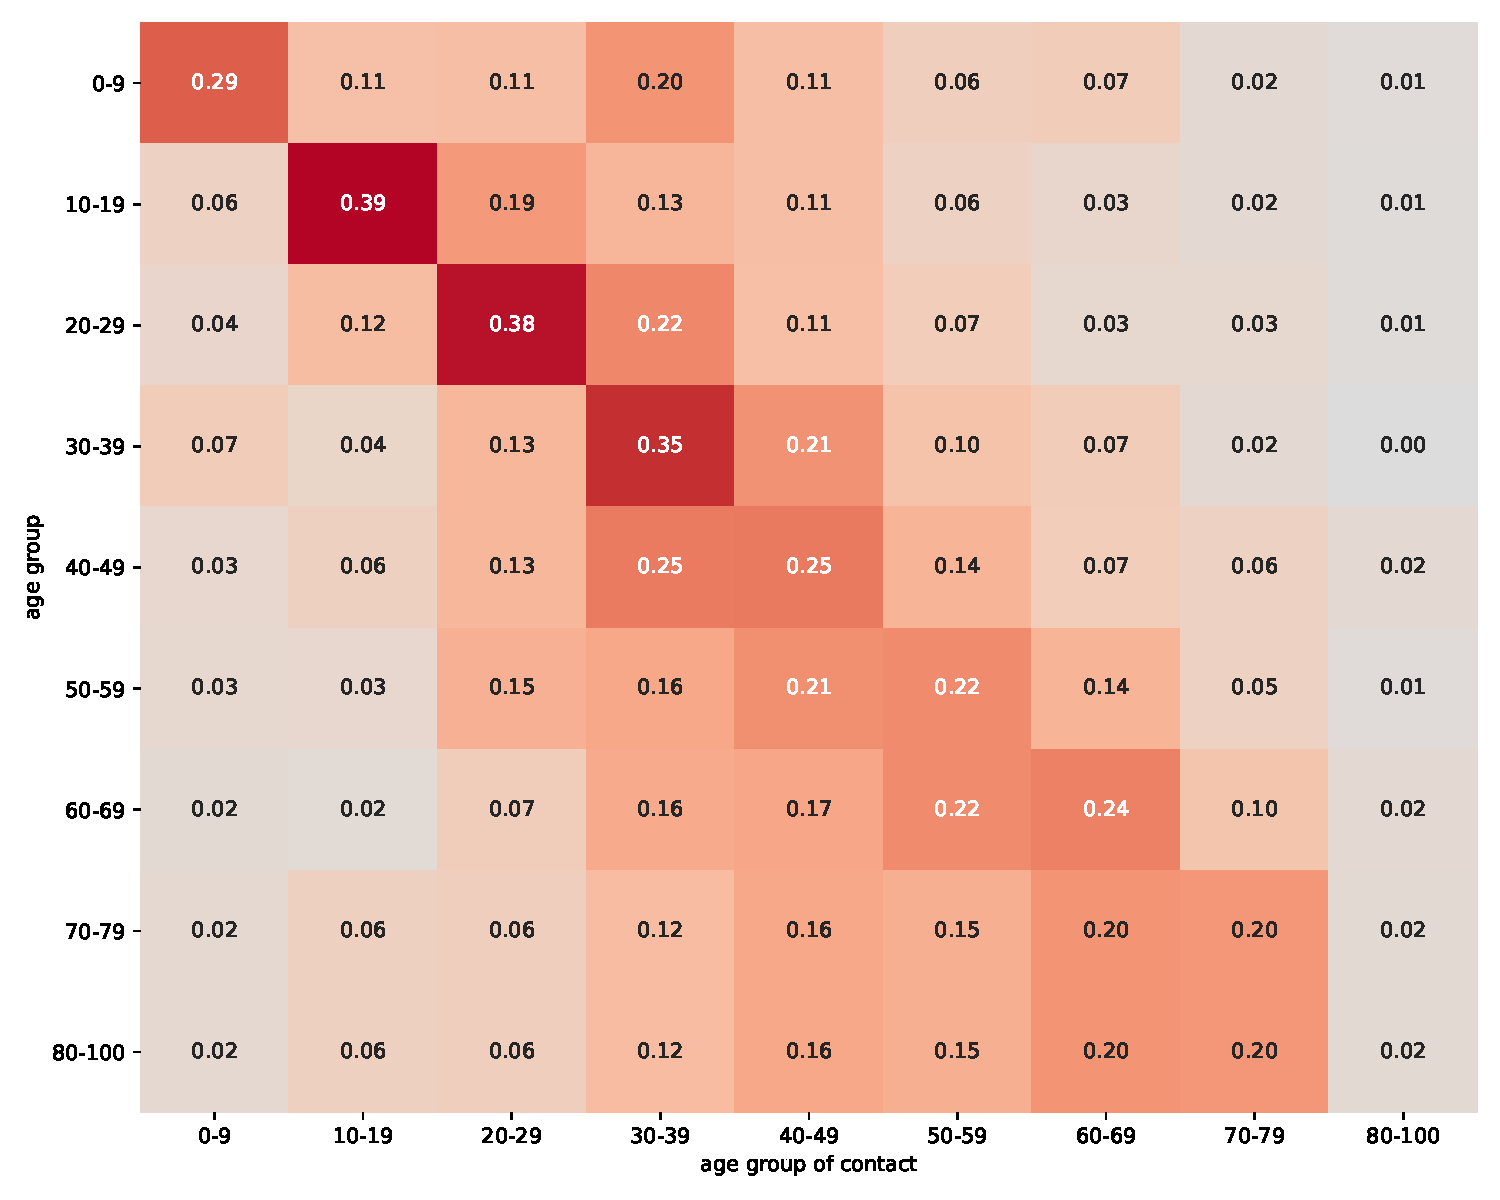
\includegraphics[width=\textwidth]{figures/results/figures/data/assortativity_other_non_recurrent}
        \caption{{Distribution of Non Recurrent Other Contacts by Age Group}}
        \label{fig:assortativity_other}
    \end{subfigure}
    \hfill
    % work assortativity
    \begin{subfigure}[b]{0.425\textwidth}
        \centering
        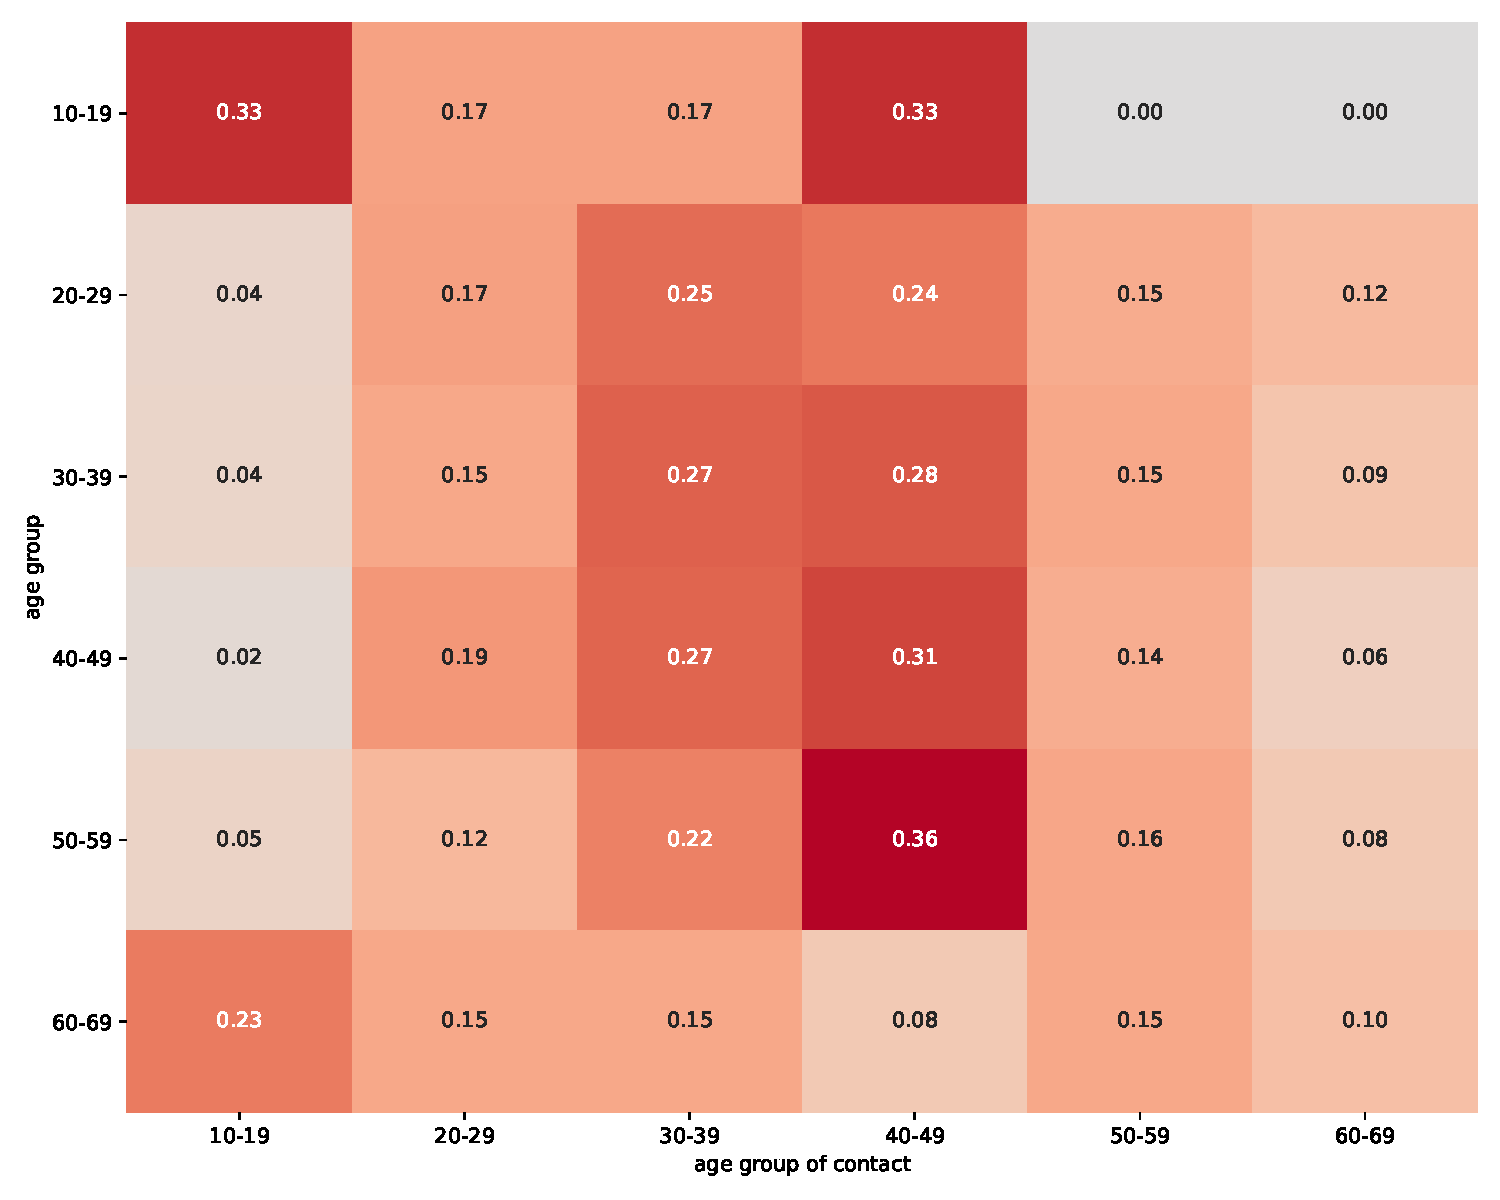
\includegraphics[width=0.9 \textwidth]{figures/results/figures/data/assortativity_work_non_recurrent}
        \caption{{Distribution of Non Recurrent Work Contacts by Age Group}}
        \label{fig:assortativity_work}
    \end{subfigure}

    \vskip3ex


    \caption{Assortativity by Age Group for Non Recurrent Other and Work Contacts}
    \floatfoot{\noindent \textit{Note:} The figure shows the distribution of non
        recurrent contacts by age group for other contacts on the left and work contacts
        on the right. A row shows the share of contacts a certain age group has with all
        other age groups. Higher values are colored in darker red tones. The diagonal
        represents the share of contacts with individuals from the same age group. The
        80-100 age group for other contacts was so small that we assumed for them to have
        the same contact distribution as the 70-79 year olds. For work contacts, we only
        show age groups that have a significant fraction of working individuals.}

    \label{fig:assortativity}

\end{figure}


Figure~\ref{fig:assortativity_other} shows that assortativity of the other contacts by
age is especially strong for children and adolescents. For older people, the pattern
becomes more dispersed around their own age group, but within-age-group contacts are
still the most common contacts. Figure~\ref{fig:assortativity_work} shows that
assortativity by age is also important among work contacts.

For recurrent contacts, we constructed groups to have the following features: Recurrent
work contacts are not assortative by age. Daily work groups are always of the same county
and weekly work contacts are to 80\% with workers from the same county. Other recurrent
contacts are constructed the same way but we impose for daily contacts that they are
always with individuals from the same age group. School classes are groups where the same
children of the mostly same age and county meet with teachers every day. Nurseries and
preschools mix children by age but match them to come mostly from the same county.
Household age composition follows directly from the German microcensus data we use to
construct our synthetic population.

\FloatBarrier

\subsection{Reducing Numbers of Contacts via NPIs}
\label{sec:policies}

Our model makes it very easy to model a wide range of NPIs, either in isolation or
simultaneously. This is important for two reasons: Firstly, it allows to predict and
quantify the effect of novel NPIs. Secondly, it allows to model the actually implemented
policy environment in great detail, which is necessary to use use the full time series
of infections and fatality rates to estimate the model parameters.\footnote{
See \citet{Avery2020} for an explanation why it can be harmful to use too long time
series to estimate simple SEIR type models.}


Instead of thinking of policies as completely replacing how many contacts people have,
it is often more helpful to think of them as adjusting the pre-pandemic number of
contacts. Therefore, we implement policies as a step that happens after the number of contacts is
calculated but before individuals are matched.

On an abstract level, a policy is a functions that modifies the number of contacts of
one contact type. This function can be random or deterministic. For example, school
closures simply set all school contacts to zero. A work from home mandate leads to a
share of workers staying home every day whereas those who cannot work from home are
unaffected. Hygiene measures at work randomly reduce the number of infectious contacts
for all workers who still go to work.

Policies can also interact. For example, school vacations are temporally reducing school
contacts to zero while at the same time increasing other contacts to account for
increased leisure activities and family visits during this time. This is important to
reproduce the finding that school vacations do not reduce infection numbers even though
schools lead to infections when open \citep{Isphording2021}.

The most complex policies are typically found in the education sector. Since the
beginning of 2021 schools have switched back and fourth between full closures,
split class approaches with alternating schedules for some or all age groups and
reopening while maintaining hygiene measures. On top of that there are different
policies for allowing young students whose parents work full time to attend school
even on days where they normally would not. For details on how we calibrate these
policies see Section~\ref{subsec:policies}.

Importantly, policies can depend on the health states of participating individuals.
This allows to quarantine entire school classes if one student tested positive or
to implement official or private contact tracing.

For some policies the exact effect on each contact type is not easy to determine. If
this refers to a policy has been active during the estimation period, it is possible to
estimate such parameters by fitting the model to time series data of infection rates.
This is only possible if the policy was not active during the whole estimation period
and thus the infection probabilities can be identified separately. We do this to account
for hygiene measures at school and in the workplace that have been in effect since
November 2020.

Not all things that reduce contacts compared to the pre-pandemic level are driven
by NPIs. Therefore, we also model endogenous contact reductions that can depend on
the health state of individuals, known risk contacts or the local incidence of
infections. Examples are strong contact reductions for symptomatic individuals or those
who have a positive PCR or rapid tests or contact reductions when a houshold member
tested positive. The extent to which contacts are reduced can be calibrated from
surveys. For an application of our model showcasing private contact tracing in the
context of the Christmas holidays see \cite{Gabler2020}.








\subsection{Rapid Test Demand}
\label{subsec:rapid_test_demand}

In our model, there are five reasons why rapid tests are done:\comment[id=J]{ Add a
    section on how we calibrate rapid test demand; Mainly describe the datapoints we have
    and say that we usually interpolate linearly in between data points. (Only exception
    to that is private rapid test demand, which we fit to data)
}

\begin{enumerate}
    \item someone plans to have work contacts
    \item someone is an employee of an educational facility or a school pupil
    \item a household member has tested positive or developed symptoms
    \item someone has developed symptoms but has not received a PCR test
    \item someone plans to participate in a weekly non-work meeting
\end{enumerate}

%%% \subsubsection{work rapid tests}

For work contacts, we know from the COSMO study (\cite{Betsch2021}, 20th/21st of April)
that 60\% of workers who receive a test offer by their employer regularly use it. We
assume this share to be time constant.

In addition, there are some surveys that allow us to trace the expansion of employers who
offer tests to their employees. Mid march, 20\% of employers offered tests to their
employees \citep{DIHK2021}. In the second half of March, 23\% of employees reported being
offered weekly rapid tests by their employer \citep{Ahlers2021}. This share increased to
61\% until the first days of April \citep{BMWI2021, IZA2021}.

Until mid April 72\% of workers were expected to receive a weekly test offer
\citep{BMWI2021, IZA2021}. However, according to surveys conducted in mid April
\citep{Betsch2021}, less than two thirds of individuals with work contacts receive a test
offer. Starting on April 19th employers were required by law to provide two weekly tests
to their employees \citep{Bundesanzeiger2021}. We assume that compliance is incomplete
and only 80\% of employers actually offer tests.

%%\subsubsection{educ rapid tests}

We assume that employees in educational facilities start getting tested in 2021 and that
by March 1st 30\% of them are tested weekly. The share increases to 90\% for the week
before Easter. At that time both Bavaria \citep{STMGP2021} and Baden-Württemberg
\citep{MinisteriumKultus2021} were offering tests to teachers and North-Rhine Westphalia
\citep{SchulministeriumNRW2021} and Lower Saxony \citep{NSMK2021} were already testing
students and tests for students and teachers were already mandatory in Saxony
\citep{SMK2021}. After Easter we assume that 95\% of teachers get tested twice per week.

Tests for students started later \citep{MinisteriumKultus2021, SchulministeriumNRW2021}
so we assume that they only start in February and only 10\% of students get tested by
March 1st. Relying on the same sources as above we approximate that by the week before
Easter this share had increased to 40\% \citep{SchulministeriumNRW2021}.

After Easter the share of students receiving twice weekly tests is set to 75\%. This is
based on tests becoming mandatory in Bavaria \citep{BayerischeStaatskanzlei2021} and
North Rhine-Westphalia \citep{SchulministeriumNRW2021b} after their Easter breaks and
on the 19th in Baden-Württemberg \citep{KMBaWue2021}.

%%\subsubsection{private rapid tests}

To limit our degrees of freedom, we only have one parameter that governs how many
individuals do a rapid test because of any of the private demand reasons (own symptoms
but no PCR test, planned weekly leisure meeting or a symptomatic or positively tested
household member).

We assume that there is no private rapid test demand until March when both the citizens'
tests and rapid tests for lay people started to become available
\citep{Bundesanzeiger2021a, Bundesregierung2021} and other access to rapid tests was very
limited.

According to the COSMO study \citep{Betsch2021a} 63\% would have been willing to take a
test in the round of 23rd of February 2021 when an acquaintance would have tested
positive. Since this is only asking for willingness not actual behavior and the demand
when meeting with friends is very likely lower, we take this as the upper bound of
private rapid test demand which is reached in the beginning of May. To cover that many
people are likely to have sought and done their first rapid test before the Easter
holidays to meet friends or family, we let the share of individuals doing rapid tests in
that time increase more rapidly than before and after. By end of March 25\% of
individuals would do a rapid test due to a private reason.

All shares of individuals who would take a rapid test if the conditions were met can be
seen in Figure~\ref{fig:rapid_test_demand}.

\begin{figure}
    \centering
    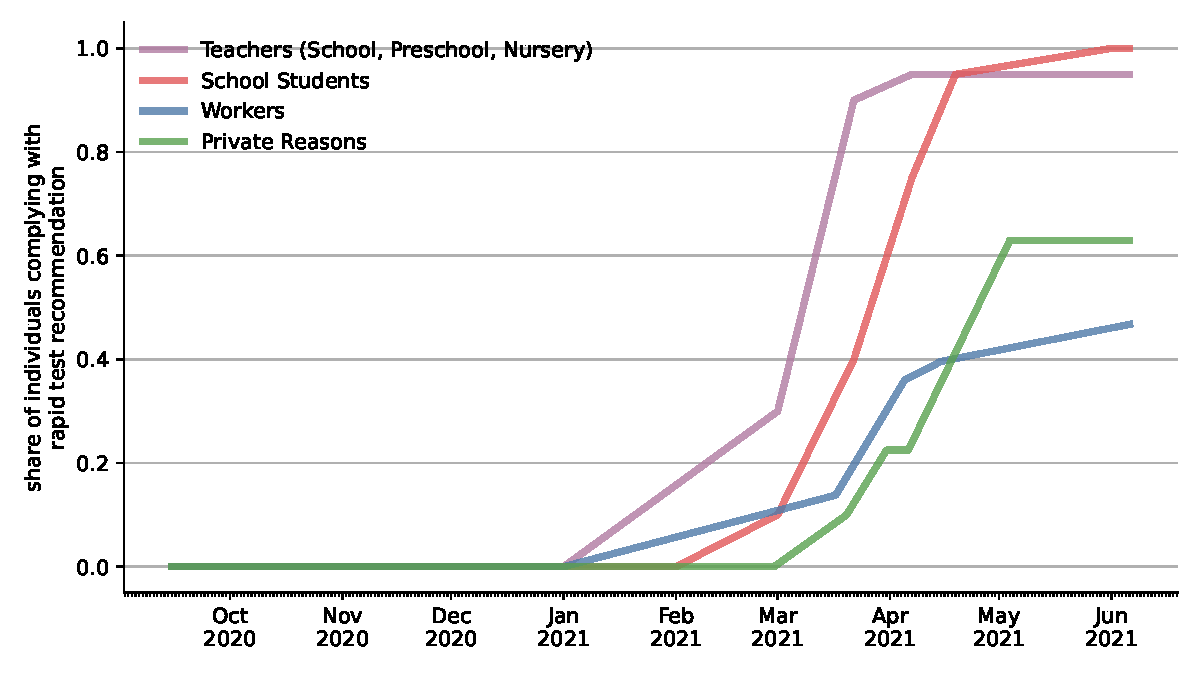
\includegraphics[width=\textwidth]{figures/results/figures/data/testing/rapid_test_demand_shares}
    \caption{\textbf{Share of Individuals Doing a Rapid Test.}}
    \floatfoot{\noindent \textit{Note:} Rapid test demand can be triggered by individuals
    planning to have education contacts, work contacts, developing symptoms without
    access to a PCR test, having a household member with a positive test or symptoms. In
    each case whether a rapid test is done depends on how long it has been since the
    individual's last rapid test and her individual compliance parameters. As an example,
    take a worker in May. In that time workers are encouraged to test themselves twice
    weekly but there is no general requirement to test themselves. If the worker has not
    done a test within the last four days in our model she will demand a test if her
    (time-constant) compliance parameter belongs to the upper 60\% in the population.}
    \label{fig:rapid_test_demand}
\end{figure}


\begin{figure}[ht]
    \centering
    \caption{Share of Individuals With Rapid Tests}
    \label{fig:share_ever_rapid_test}
    \begin{subfigure}{.55\textwidth}
        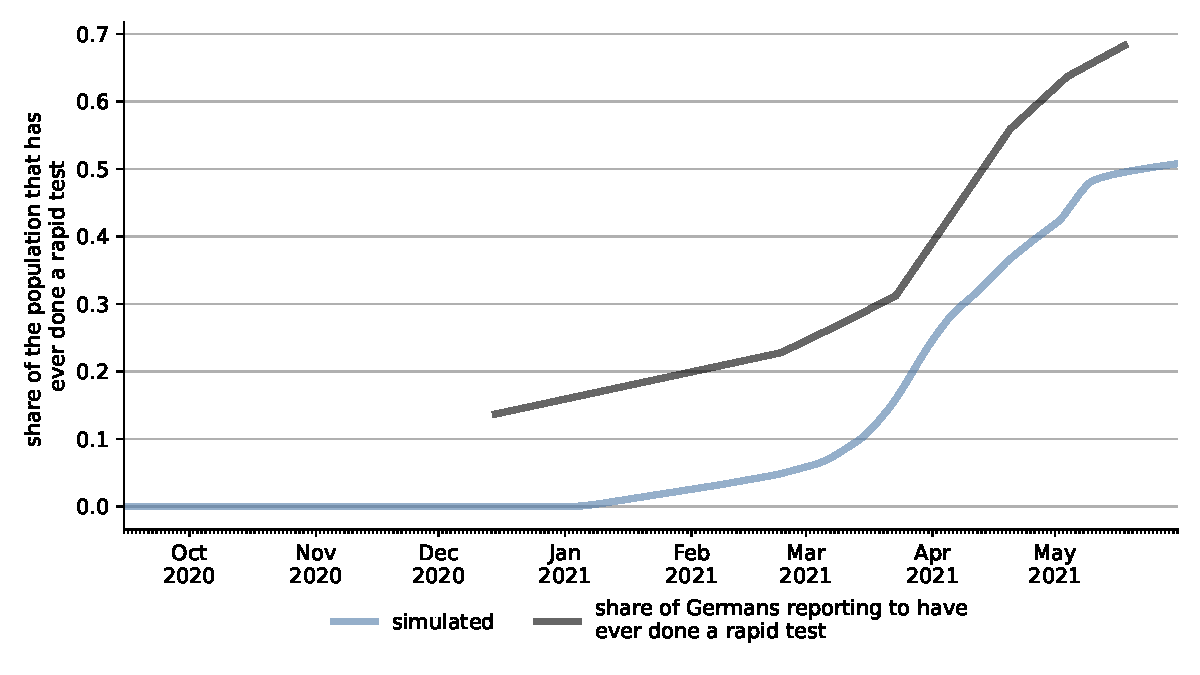
\includegraphics[width=0.9 \textwidth]{figures/results/figures/scenario_comparisons/combined_fit/full_share_ever_rapid_test}
        \caption{Share of Individuals That Have Ever Done a Rapid Test}
    \end{subfigure}%
    \begin{subfigure}{.55\textwidth}
        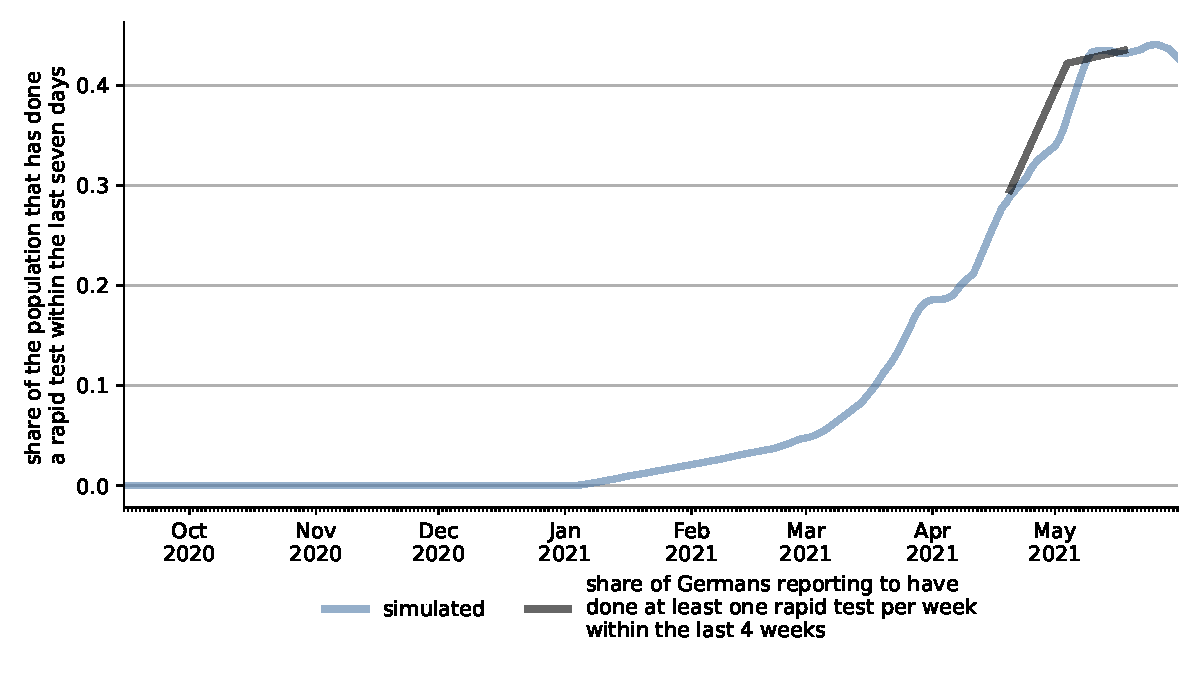
\includegraphics[width=0.9 \textwidth]{figures/results/figures/scenario_comparisons/combined_fit/full_share_rapid_test_in_last_week}
        \caption{Share of Individuals Having Done a Rapid Test in the Last Week}
    \end{subfigure}
    \label{fig:share_rapid_test_last_week}
    \floatfoot{\noindent \textit{Note:} The figure compares the share of individuals who
        have ever done a rapid test or done a rapid test within the last week in our
        simulations to the shares reported in the
        \href{https://projekte.uni-erfurt.de/cosmo2020/web/topic/wissen-verhalten/80-schnelltests/}{COVID-19
        Snapshot Monitoring Survey}. The left panel compares the share of individuals who
        have ever done a rapid test. The right panel compares the share of individuals
        who have done a rapid test within the last seven days in our simulation compared
        to the share reporting to have done at least weekly rapid tests in the last four
        weeks in the COSMO survey. Overall our calibration of rapid tests are slightly
        conservative. The overall share is below that in the study. We fit the share of
        weekly tests quite exactly. However, the study only covers adults while our share
        also includes children who are tested very regularly when attending school.}
\end{figure}

 \comment[id=K]{J: Explain that we don't fit the share ever tested that well because our rapid test compliance is completely fixed. }

\FloatBarrier

\subsection{Share of Detected Cases}
\label{subsec:data_share_known_cases}

One important feature of our model is that we distinguish between undetected and detected
cases and that we model which cases are detected and which are not (see
Section~\ref{sub:testing} for a detailed description for how we model both rapid and PCR
tests). For our model it is important to have an estimate for the share of cases that is
detected in the absence of rapid tests ($\psi_t$). For this we rely on the
\cite[Dunkelzifferradar Project][]{Dunkelzifferradar2020} which uses estimates of the
case fatality rate to estimate the number of total cases given the number of CoViD-19
deaths which are assumed to be perfectly observable. For 2020, we follow the reported
share of detected cases quite closely. One exception is the phase of November 2020 where
we interpolate to maintain monotonicity during the fall as there was no reason why the
share of detected cases should have risen in that time\footnote{The testing policy
changed in November \citep{RKI2020a}. However, this only moved the rare PCR tests more
towards vulnerable groups.}

% After Christmas 2020
Since vaccinations started after Christmas 2020 and these were predominantly given to
nursing homes in the beginning and other vulnerable groups in spring, we expect the
relationship between deaths and the number of total infections to change rapidly in 2021.
This is why we stop using the share of detected cases estimated by the Dunkelzifferradar
after Christmas. Instead, we assume that the share of detected cases would have stayed
the same in the absence of rapid tests. Thus, we also achieve in our model an increase in
the share of detected cases but this is driven from inside our model through increased
rapid testing which lead follow-up PCR tests when they are positive (see
Section~\ref{subsec:results_share_known_cases} and \ref{sub:testing}).

% Christmas and Easter
Lastly, we model reductions in the share of detected cases due to the two major holidays in our
simulation period, Christmas and Easter. During both holidays many laboratories did not
process tests and most physicians' offices were closed, leading to less PCR tests and
short and large drops in the share of known cases. The resulting share of detected cases
in the absence of rapid tests is shown in Figure~\ref{fig:share_known_cases_data} and
was estimated to fit the data.

\begin{figure}[ht]
  \centering
  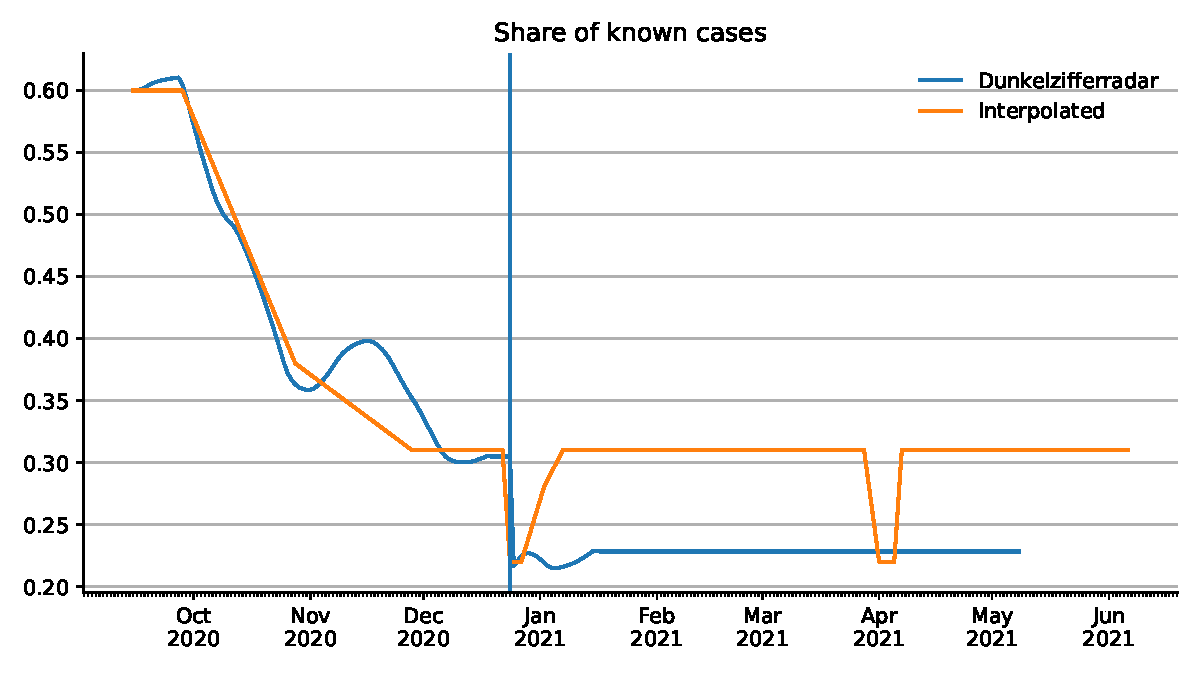
\includegraphics[width=0.5\textwidth]{figures/results/figures/data/testing/assumed_overall_share_known_cases}
  \caption{Share of Detected Cases in the Absence of Rapid Tests}
  \label{fig:share_known_cases_data}
  \floatfoot{\noindent \textit{Note:} The figure shows the share of cases that is
  reported as an official case via PCR confirmation. We use the overall share of known
  cases that was estimated through the case fatality ratio by the \cite[Dunkelzifferradar
  Project][]{Dunkelzifferradar2020} for all of 2020 and then assume it to be constant as
  vaccinations of the elderly strongly affect the case fatality rate which the project
  does not account for. Starting in 2021 in addition to the overall numbers of detected
  cases through symptoms and a random component, cases are also detected through
  confirmation of positive rapid tests which happens endogenously inside the model. For
  the public holidays of Christmas and Easter we lower the share of detected cases as
  fewer PCR tests are available during public holidays. See
  Figure~\ref{fig:share_known_cases_by_age_group} for how the share of detected cases
  develops in our model for each age group}.
\end{figure}

\FloatBarrier


\subsection{PCR Testing and Behavioral Response}
\label{subsec:pcr_testing_and_behavioral_response}

 \comment[id=K]{@Janos: Read this}

After showing how we calibrate rapid test demand and the share of detected cases, this
section describes the remaining parameters for our testing model. Refer to
Section~\ref{sub:testing} for a description of the full testing model.

% share of tests for symptomatics
From the share of detected cases and the number of infections we arrive at the number of
positive PCR tests in our model. A share of these positive tests is given to symptomatic
individuals ($\chi_{symptom,\:t}$). This share is calibrated from German data on case
characteristics \citep{RKICaseCharacteristics} and shown in
Figure~\ref{fig:share_pcr_to_symptomatic}. We keep $\chi_{symptom,\:t}$ constant after
Christmas because the RKI data does not include if a PCR test was done to confirm a
positive rapid test and this share is used for PCR test demand without prior rapid test
indication

\begin{figure}
    \centering
    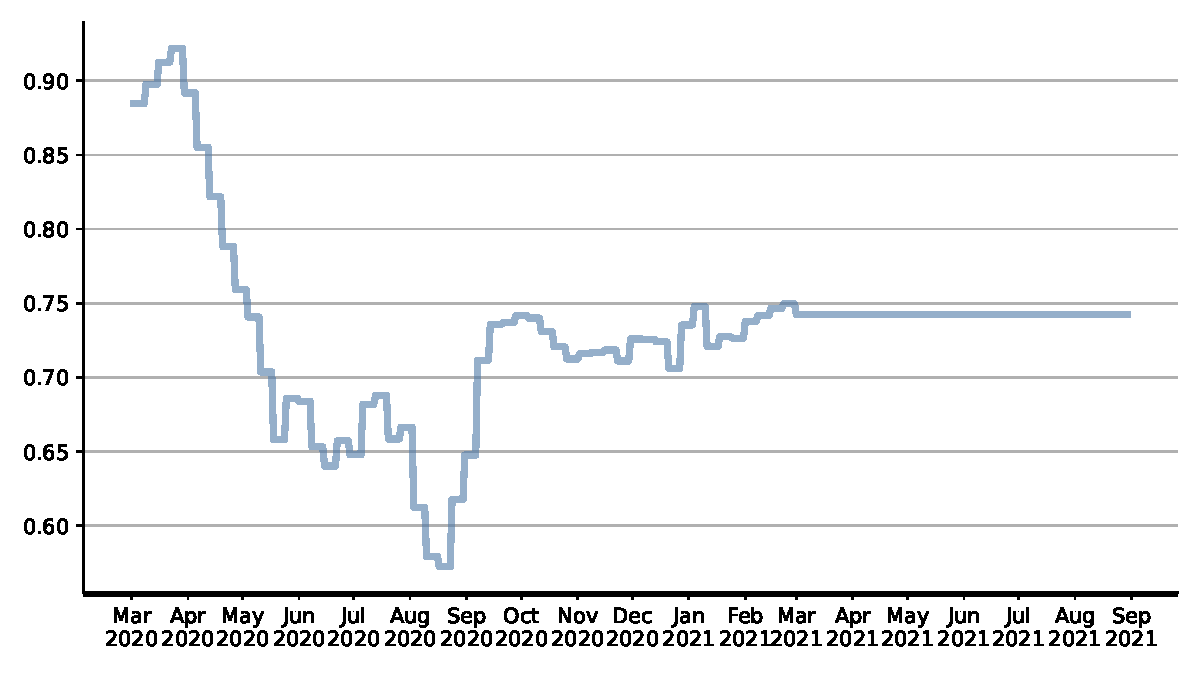
\includegraphics[width=0.5\textwidth]{figures/results/figures/data/testing/used_share_of_pcr_tests_going_to_symptomatics}
    \caption{Share of Positive PCR Tests Administered to Symptomatic Individuals}
    \label{fig:share_pcr_to_symptomatic}
    \floatfoot{\noindent \textit{Note:} The share of positive PCR tests that are
    administered to symptomatic individuals ($\chi_{symptom,\:t}$). Since it was not
    recorded for every case if the person was symptomatic or not we take the midpoint
    between the upper and lower bound. We keep the share constant after Christmas because
    the RKI data does not include if a PCR test was done to confirm a positive rapid test
    and this share is used for PCR test demand without prior rapid test indication.}
\end{figure}

% time until test result
PCR tests take one to four days until their result is revealed to the individual
($\gamma_{PCR,\:d}$). Relying on the ARS data \citep{ARS2020} we calculate that 33\% of
individuals receive the test result after one day, 50\% after two days, 10\% after three
days and 7\% after four days.

% share with positive rapid test requesting pcr
To model the demand for PCR tests through rapid tests, we only need the share of
individuals that seek a PCR test to confirm a positive rapid test result
($\chi_{confirmation}$). We calibrate this from \citet{Betsch2021} who asked this
hypothetical question in March of 2021. There 82\% of Germans reported that they would
follow up on a positive rapid test with a PCR test.

% Behavioral Response ------------------------------------------------------------------

Lastly, we need to set the parameters that decide how individuals reduce their contacts
after certain events, $\tau$. We distinguish between the reduction in household contacts
(which are harder to avoid) and non household contacts. There are three events which
trigger potential contact reductions: showing symptoms of CoViD-19, having received a
positive rapid test and having received a positive PCR test. The only survey data we are
aware of on this is \citet{Betsch2021} where 85\% of individuals claimed they
would isolate and restrict their contatcs after a positive rapid test. We assume this
reduction for non household contacts. As household contacts are much more difficult to
avoid, we assume that they are only reduced by 30\%. We assume the same behavior for
individuals that develop symptoms. Lastly, we assume the response to a positive PCR test
to be stronger than in the other two cases and set the reduction of non household
contacts to 95\% and the reduction of household contacts to 50\%.

\FloatBarrier

\subsection{Estimated Parameters}
\label{subsec:estimated_params}

%%% The free parameters are the infection probabilities by contact category, one hygiene
%%% multiplier for school and work contacts after November 2nd 2020, approx. ten parameters
%%% that govern the reduction of other contacts\comment[id=K]{Must be updated when the
%%% estimation is finished.}, the number of extra contacts during holidays, the share of
%%% detected cases around holidays and the fade in speed of the rapid tests as well as one
%%% parameter that governs the import of B.1.1.7 cases in January 2021.



\FloatBarrier

% infection probabilities

To calibrate infection probabilities outside of the model, it would be important to know
the exact duration and distance of each contact type as well as viral loads. Since this
is not available in any data set, we estimate those parameters inside the model with the
method of simulated moments \citep{McFadden1989} by minimizing the distance between
simulated and observed infection rates. Since our model includes a lot of randomness, we
average simulated infection rates over several model runs.

We use data for Germany from October 2020 until June 2021. We do not use
earlier periods for three reasons. Firstly, in the beginning PCR tests were highly
limited and therefore it would be difficult to find good initial conditions for our
simulations. In addition during the summer the case numbers were extremely low. This
could lead to the epidemic going extinct in our simulation. Additionally, our model does
not include international travel or other imports of cases. These would be important but
difficult to model during the summer months.

To avoid over-fitting and simplify the numerical optimization problem, we only allow for
five different probabilities: 1) for contacts in schools 2) contacts in preschools and
nurseries. 3) for work contacts. 4) for households. 5) for other contacts.

The infection probabilities estimated from our model are as follows: For household
contacts (each individual meets all his or her household members every day) the infection
probability is 10\%, for school contacts (all students and teachers meet all other
students and teachers that attend school that day and there are three classes taking
place each day) the probability of infection is 1.2\%, for preschools and nurseries that
infection probability is 0.5\%. Work contacts carry a risk of 14.5\% and other activities
(including leisure activities such as meeting friends) carry the highest risk with
15.875\%.\comment[id=HM]{Are these numbers current? In any case, a table would substitute for this and the previous paragraph. Need to mention B.1.1.7 alongside.}\comment[id=K]{Missing to add data for the other estimated parameters (import of b117 etc)}


\subsection{Shapley Values} % (fold)
\label{sub:shapley_value}

We decompose the effects of different NPIs and seasonality on the infection rates with
Shapley values. Shapley values \citep{Shapley2016} are a concept in game theory to
divide payoffs between a coalition of players. It allows to assign a single value to the
contribution of an NPI or seasonality which takes into account substitutional and
complementary effects with other factors.

More formally, define a coalitional game with $N$ players and a super-additive function
$\nu$ which maps subsets of $N$ to the real numbers. The function $\nu$ is also called
the characteristic function and assigns a value to a coalition. Then, the Shapley value
$\phi$ for player $i$ is

\begin{align*}
    \phi_i(\nu) = \frac{1}{|N| !} \sum_{S \subseteq N \setminus \{i\}} |S| ! (|N| - |S| - 1)! (\nu(S \cup \{i\}) - \nu(S))
\end{align*}

The last term $(\nu(S \cup \{i\}) - \nu(S))$ is the marginal contribution of player $i$
minus the coalition without player $i$. Then, compute the sum of marginal contributions
over all subsets $S$ of $N$ which do not include player $i$. Each marginal contribution
has to be multiplied by all combinations of other players in $S$ which precede $i$ and
all possible combinations of remaining players which follow player $i$ in the coalition.
To arrive at the Shapley value for player $i$, divide the sum by the total number of
combinations.

The Shapley value has some properties.

\begin{description}
  \item[Efficiency] The sum of Shapley values is equal to the value of a coalition
  formed by all players.
  \item[Symmetry] The Shapley does not depend on the label of a player but only on its
  position in the characteristic function.
  \item[Linearity] The Shapley value depends linearly on the values from the
  characteristic function $\nu$.
  \item[Dummy Axiom] The Shapley value of a player who contributes nothing to any
  coalition is 0.
\end{description}

To produce Figure~\ref{fig:2021_scenarios_decomposition} and
Figure~\ref{fig:2021_scenarios_decomposition_tests}, we calculate the Shapley values of
each factor in the comparison on the cumulative number of saved infections between the
main scenario and the scenario without any of the factors for every day. Then, we divide
up the saved infections on a particular day according to the Shapley values for the same
day which yields the daily saved infections for each factor.


% subsection shapley_value (end)

\clearpage

\begin{landscape}

\subsection{Overview Model Parameters} % (fold)
\label{sub:param_tables}

 \comment[id=K]{@Janos: Double check this.}


\FloatBarrier

\begin{table}[htb]
\centering
\caption{Contacts, Matching and Policies}
\label{tab:contacts_and_matching}
\input{../bld/param_tables/contacts_matching_policies}
\end{table}


\begin{table}[htb]
\centering
\caption{Infection Probabilities and Virus Variants}
\label{tab:infection_probs}
\input{../bld/param_tables/infection_probs}
\end{table}


\begin{table}[htb]
\centering
\caption{Disease and Vaccination Model}
\label{tab:disease_and_vacc_model}
\input{../bld/param_tables/disease_model}
\end{table}


\begin{table}[htb]
\centering
\caption{Rapid Testing}
\label{tab:rapid_testing}
\input{../bld/param_tables/rapid_testing}
\end{table}


\begin{table}[htb]
\centering
\caption{PCR Testing, Case Detection and Behavioral Response}
\label{tab:pcr_testing_and_case_detection}
\input{../bld/param_tables/pcr_testing_and_case_detection}
\end{table}

\FloatBarrier

\end{landscape}

\FloatBarrier


\subsection{Reproducibility}
\label{subsec:code}

The source code used for this paper is open source and available under the MIT License.
It is split into two parts
\begin{itemize}
    \item The source code for the model can be found at
   \href{https://github.com/covid-19-impact-lab/sid/}{https://github.com/covid-19-impact-lab/sid/}
   and its documentation at
   \href{https://sid-dev.readthedocs.io}{https://sid-dev.readthedocs.io}.
   \item The source code for the application to Germany can be found at
   \href{https://github.com/covid-19-impact-lab/sid-germany/}{https://github.com/covid-19-impact-lab/sid-germany/}
   with a shorter documentation at
   \href{https://sid-germany.readthedocs.io}{https://sid-germany.readthedocs.io}.
\end{itemize} 

We are grateful to the authors and contributors of the following software packages upon
which our software is built: conda \cite{Anaconda2016}, conda-forge
\cite{CondaForge2015} dask \cite{Rocklin2015}, estimagic \cite{Gabler2020a}, holoviews
\cite{Stevens2015}, matplotlib \cite{Hunter2007}, numba \cite{Lam2015}, numpy
\cite{Harris2020}, pandas \cite{Reback2020,McKinney2010}, pytask \cite{Raabe2020},
Python \cite{VanRossum1995}, scipy \cite{Virtanen2020}.


        \FloatBarrier

        \section{Supplementary Text}
\label{sec:supplementary_text}

% Model

\subsection{Literature Review}
\label{sec:literature_review}

We build on two strands of literature: Recent extensions of the epidemiological SEIR
model and agent-based simulation models.

The traditional SEIR model is not fine-grained enough to model nuanced policies. This
has motivated a large number of researchers to extend the standard model to allow for
more heterogeneity and flexibility. Examples are \citet{Grimm2020},
\citet{Donsimoni2020} and \citet{Acemoglu2020} who develop multi group SEIR models to
analyze the effects of targeted lockdowns and \citet{Berger2020} who extend the SEIR
model to analyze testing and conditional quarantines. For a more comprehensive review
see \citet{Avery2020}. Others have used the results of a standard SEIR model as input
for economic models that estimate the cost of policies (e.g. \citet{Dorn2020}).

While the popularity of the SEIR model is mainly due to its simplicity, the extensions
are quite complex. It is unlikely that there will be a SEIR model that combines all
proposed extensions. Moreover, the extensions do not address other key issues: The main
parameter of the SEIR model, the basic reproduction number ($R_0$), is not
policy-invariant. It is a composite of the number of contacts each person has and the
infection probability of the contacts. In fact, policy simulations are done by setting
$R_0$ to a different value but it is hard to translate a real policy into the value of
$R_0$ it will induce. In other words, SEIR models are not suited for evaluating the
effect of policies which have never been experienced before.

Another commonly used model class in epidemiology are agent-based simulation models. In
these models individuals are simulated as moving particles. Infections take place when
two particles come closer than a certain contact radius (e.g. \citet{Silva2020} and
\citet{Cuevas2020}). While the simulation approach makes it easy to incorporate
heterogeneity in disease progression, it is hard to incorporate heterogeneity in meeting
patterns. Moreover, policies are modeled as changes in the contact radius or momentum
equation of the particles. The translation from real policies to corresponding model
parameters is a hard task.

\citet{Hinch2020} is a recent extension of the prototypical agent-based simulation model
that replaces moving particles by contact networks for households, work and random
contacts. This model is similar in spirit to ours but focuses on contact tracing rather
than social distancing policies.

The above assessment of epidemiological models is not meant as a critique. We are aware
that these models were not designed to predict the effect of fine-grained social
distancing policies in real time and are very well suited to their purpose. We invite
epidemiologists to provide feedback and collaborate to improve our model.


\subsection{Summary}
\label{sub:model_summary}

To alleviate these problems we propose a different model structure. Our model inherits many features from agent-based simulation models but replaces the contacts between moving particles by contacts between individuals who work, go to school, live in a household and enjoy leisure activities. The structure of the model is depicted in Figure~\ref{fig:model_graph}.

\begin{figure}[!ht]
    \centering
    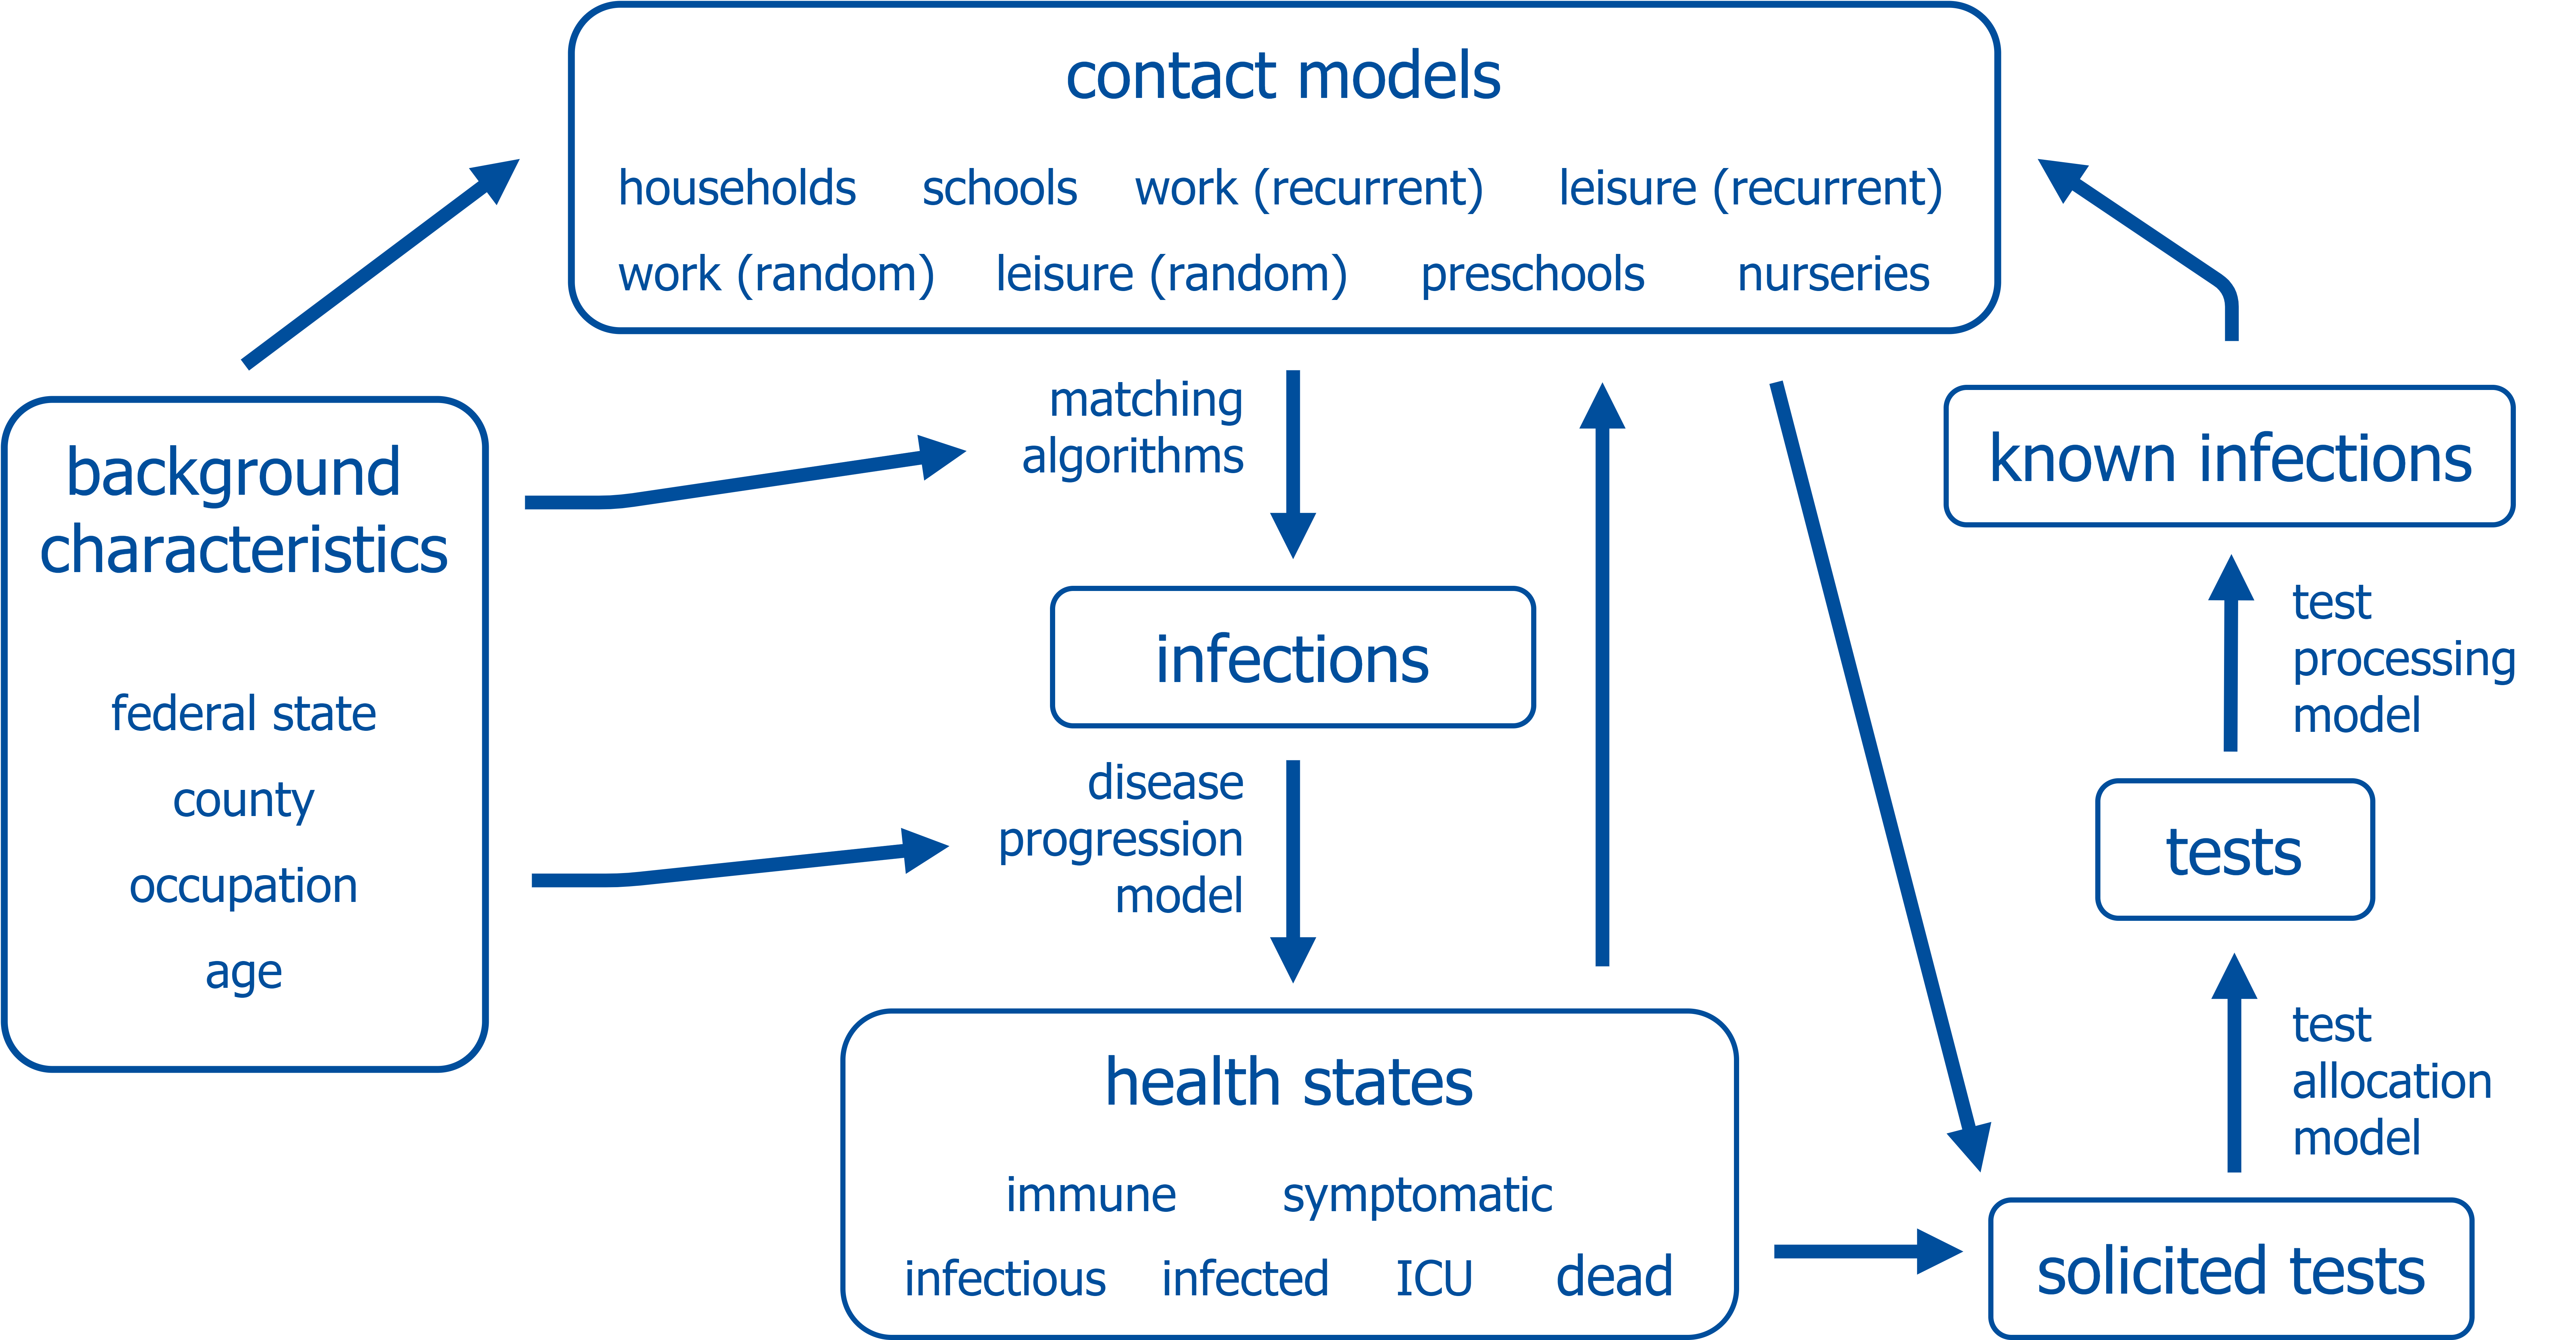
\includegraphics[width=0.7\textwidth]{../figures/model_detailed.png}
    \caption{Simplified graph of the model}
    \label{fig:model_graph}
\end{figure}

The background characteristics include age, county and occupation of each simulated individual. Contact models are functions that map individual characteristics into a predicted number of contacts. Currently we distinguish between eight types of contact models which are all listed in Figure~\ref{fig:model_graph}: households, recurrent and random work contacts, recurrent and random leisure contacts, and nursery, preschool, and school contacts.

The predicted number of contacts is translated into infections by a matching algorithm. There are different matching algorithms for recurrent contacts (e.g. classmates, family members) and non-recurrent contacts (e.g. clients, contacts in supermarkets). The infection probability can differ for each contact type. All types of contacts can be assortative with respect to geographic and demographic characteristics.

Once a person is infected, the disease progresses in a fairly standard way which is also depicted in Figure~\ref{fig:course_of_disease}. Asymptomatic cases and cases with mild symptoms are infectious for some time and recover eventually. Cases with severe symptoms additionally require hospitalization and lead to either recovery or death.

There are two possible ways to enable testing for Covid-19 in the model. The first way allows to specify the ratio of known to unknown infections for each day. A random sample of all newly infected individuals will then receive a test result in the following days. The second approach consists of three steps. First, individuals demand a test because they, e.g., experience symptoms. Secondly, tests are allocated to individuals while respecting governmental access restrictions to test. Thirdly, depending of the capacities of laboratories, tests are processed for some time until the individual receives her test result.

In addition, people who have symptoms, received a positive test, or had a risk contact can reduce their number of contacts across all contact types endogenously.

The model makes it very simple to translate policies into model quantities. For example, school closures imply the complete suspension of school contacts. A strict lockdown implies shutting down work contacts of all people who are not employed in a systemically relevant sector. It is also possible to have more sophisticated policies that condition the number of contacts on observable characteristics, risk contacts or health states.

Another key advantage of the model is that the number of contacts an individual has of each contact type can be calibrated from publicly available data \citep{Mossong2008}. This in turn allows us to estimate policy-invariant infection probabilities from time series of infection and death rates using the method of simulated moments \citep{McFadden1989}. Since the infection probabilities are time-invariant, data collected since the beginning of the pandemic can be used for estimation. Moreover, since we can model the testing strategies that were in place at each point in time, we can correct the estimates for the fact that not all infections are observed.

Last but not least, performing simulations whose starting point is set amidst the pandemic requires special adjustments to arrive at a realistic distribution of courses of diseases. We solve the initial conditions problem by matching reported infections to individuals in our data while also correcting for reporting lag and undetected cases.

In the following sections we describe each of the model components in more detail.


\subsection{Modeling Numbers of Contacts}
\label{sec:number_of_contacts}

Consider a hypothetical population of 1,000 individuals in which 50 were infected with a novel infectious disease. From this data alone, it is impossible to say whether only those 50 people had contact with an infectious person and the disease has an infection probability of 1 in each contact or whether everyone met an infectious person but the disease has an infection probability of only 5 percent per contact. SEIR models do not even try to distinguish contact frequency from the infectiousness of each contact and combine the two in one parameter that is not invariant to social distancing policies.

To model social distancing policies, we need to disentangle the effects of the number of contacts of each individual and the effect of policy-invariant infection probabilities specific to each contact type. Since not all contacts are equally infectious, we distinguish different contact types.

The number and type of contacts in our model can be easily extended. Each type of contacts is described by a function that maps individual characteristics, health states and the date into a number of planned contacts for each individual. This allows to model a wide range of contact types.

Currently, there are the following contact types:

\begin{itemize}
    \item Households: Each household member meets all other household members every day. The household sizes and structures are calibrated to be representative for Germany.

    \item Random non-work contacts: Each person has contacts with randomly drawn other people which are assortative with respect to region and age group. This contact type reflects contacts during pure leisure activities as well as non leisure activities such as grocery shopping or medical appointments.

    \item Recurrent daily non-work contacts: Each person has daily recurring contacts which allows to model close relationships other than families between individuals.

    \item Recurrent weekly non-work contacts: Each person has weekly recurring contacts like sports groups or other weekly activities.

    \item Random work contacts: Each working adult has contact to randomly drawn other people at work.

    \item Recurrent daily work contacts: Each working adult meets other workers every day. This is meant to capture work colleagues.

    \item Recurrent weekly work contacts: Each working adult meets other workers once per week. We randomize over the days on which the meetings take place. This is meant to capture meetings with clients, superiors or other colleagues which happen infrequently.

    \item Schools: Each student meets all of his classmates every day. Class sizes are calibrated to be representative for Germany and students have the same age. Schools are closed on weekends and during vacations, which vary by states. School classes also meet three pairs of teachers every school day. The pairs are meant to represent interactions between teachers.

    \item Preschools: Children who are at least three years old and younger than six may attend preschool. Each group of nine children interacts with the same two adults every day. The children in each group are of the same age. The remaining mechanics are similar to schools.

    \item Nurseries: Children younger than three years may attend a nursery and interact with one adult. The age of the children varies within groups. The remaining mechanics are similar to schools.
\end{itemize}

The number of random and recurrent contacts at the workplace and at home is calibrated with data provided by \cite{Mossong2008}. For details see Section~\ref{sec:calibration}. In particular, we sample the number of contacts or group sizes from empirical distributions that sometimes depend on age. Instead it would also be possible to use economic or other behavioral models to predict the number of contacts.

Theoretically, each contact type can have its own infection probability. However, to reduce the number of free parameters and thus avoid a potential over-fitting we impose some constraints. For now, infection probabilities in schools, preschools and nurseries are equal. Moreover, we restrict all work contacts to have the same infection probability. ???STILL TRUE???


\subsection{Reducing Numbers of Contacts Through Policies}
\label{sec:policies}

The main motivation of our model is to predict the effect of policies that affect the
number of contacts people have. Examples range from school closures and lockdowns to
more nuanced policies such as mandatory quarantines for symptomatic individuals or a
class splitting policy where only half of the students come to school in person and the
other half joins digitally with weekly rotation.

Instead of thinking of policies as completely replacing how many contacts people have,
it is often more helpful to think of them as adjusting the pre-pandemic number of
contacts.

Therefore, we implement policies as a step that happens after the number of contacts is
calculated but before individuals are matched.

On an abstract level, a policy is a functions that modifies the number of contacts of
one contact type. For example, school closures simply set all school contacts to zero. A
lockdown where only essential workers are allowed to work means that approximately two
thirds of the working population have zero work contacts and the rest has the same
number of contacts as before.

This, in conjunction with our fine-grained contact types, allows us to easily implement
a wide variety of policies. Allowing policies to depend on the health states of the
entire population means that adaptive lockdowns where, for example, schools close when a
certain threshold of infections is surpassed at the county level would be as simple as
determining which counties are above the threshold and then setting all school contacts
in these counties to zero.

The dependency of policies on health states also makes it possible to model contact
tracing. For example, a policy could check whether each child has a classmate who's
received a positive test result and then bar all children of that class from attending
school.

Some policies can be easily implemented if the background characteristics are suitably
extended. For example, a schooling policy of splitting and rotating classes,
where each half attends school every other week can be implemented by storing
whether the child would attend in even or odd weeks in the background characteristics
and then using that information in the policy function.

For some policies the exact effect on each contact type is not easy to determine. If
this refers to a policy during the estimation period, it is possible to estimate such
parameters by fitting the model to time series data of infection rates. This is only
possible if the policy was not active during the whole estimation period and thus the
infection probabilities can be identified separately. If instead it refers to a policy
that we want to simulate, we make a scenario analysis in which the model is simulated
with several assumptions about how the policy affects the number of contacts.


\subsection{Matching Individuals}
\label{sec:matching}

The empirical data described above only allows to estimate the number of contacts each person has. In order to simulate transmissions of Covid-19, the numbers of contacts has to be translated into actual meetings between people. This is achieved by matching algorithms:

As described in section \ref{sec:number_of_contacts}, some contact types are recurrent (i.e. the same people meet regularly), others are non-recurrent (i.e. it would only be by accident that two people meet twice). The matching process is different for recurrent and non recurrent contact models.

Recurrent contacts are described by two components: 1) A variable in the background characteristics. An example would be a school class identifier which could come from actual data or be drawn randomly to achieve representative class sizes. 2) A deterministic or random function that takes the value 0 (non-participating) and 1 (participating) and can depend on the weekday, date and health state. This can be used to model vacations, weekends or symptomatic people who stay home (see section \ref{sec:endogenous_contact_reductions} for details).

The matching process for recurrent contacts is then extremely simple: On each simulated day, every person who does not stay home meets all other group members who do not stay home. The assumption that all group members have contacts with all other group members is not fully realistic, but seems like a good approximation to reality, especially in light of the suspected role of aerosol transmission for Covid-19 (\cite{Morawska2020, Anderson2020}).

The matching in non-recurrent contact models is more difficult and implemented in a two stage sampling procedure to allow for assortative matching. Currently most contact models are assortative with respect to age (it is more likely to meet people from the same age group) and county (it is more likely to meet people from the same county) but in principle any set of discrete variables can be used. This set of variables that influence matching probabilities introduce a discrete partition of the population into groups. The first stage of the two stage sampling process samples on the group level. The second stage on the individual level.

Below, we first show pseudo code for the non-recurrent matching algorithm and then describe how the algorithm works in words.

%%% ToDo: Get syntax highlighting for the pseudo code. Try out different languages.

\begin{lstlisting}
while unmatched contacts remain:
    model, id = draw contact model and individual
    for contact in remaining_contacts[id, model]:
        draw group of other person
        draw other person from that group
        determine if id infects other or vice versa
        remaining_contacts[id, model] -= 1
        remaining_contacts[other, model] -= 1
\end{lstlisting}


We first randomly draw a contact type and individual. For each contact oth the drawn contact type that person has, we first draw the group of the other person (first stage). Next, we calculate the probability to be drawn for each member of the group, based on the number of remaining contacts. I.e. people who have more remaining contacts are drawn with a higher probability. This has to be re-calculated each time because with each matched contact, the number of remaining contacts changes. We then draw the other individual, determine whether an infection takes place and if so update the health states of the newly infected person. Finally, we reduce the number of remaining contacts of the two matched individuals by one.

The recalculation of matching probabilities in the second stage is computationally intensive because it requires summing up all remaining contacts in that group. Using a two stage sampling process where the first stage probabilities remain constant over time makes the matching computationally much more tractable because the number of computations increases quadratically in the second stage group size.


\FloatBarrier

\subsection{Course of the Disease}
\label{sub:course_of_disease}

The following medical parameters describing the progression of the disease are taken from systematic reviews (e.g. \citet{He2020}). After an infection occurs, the disease progresses in the way depicted in Figure~\ref{fig:course_of_disease}.

\begin{figure}[!tp]
    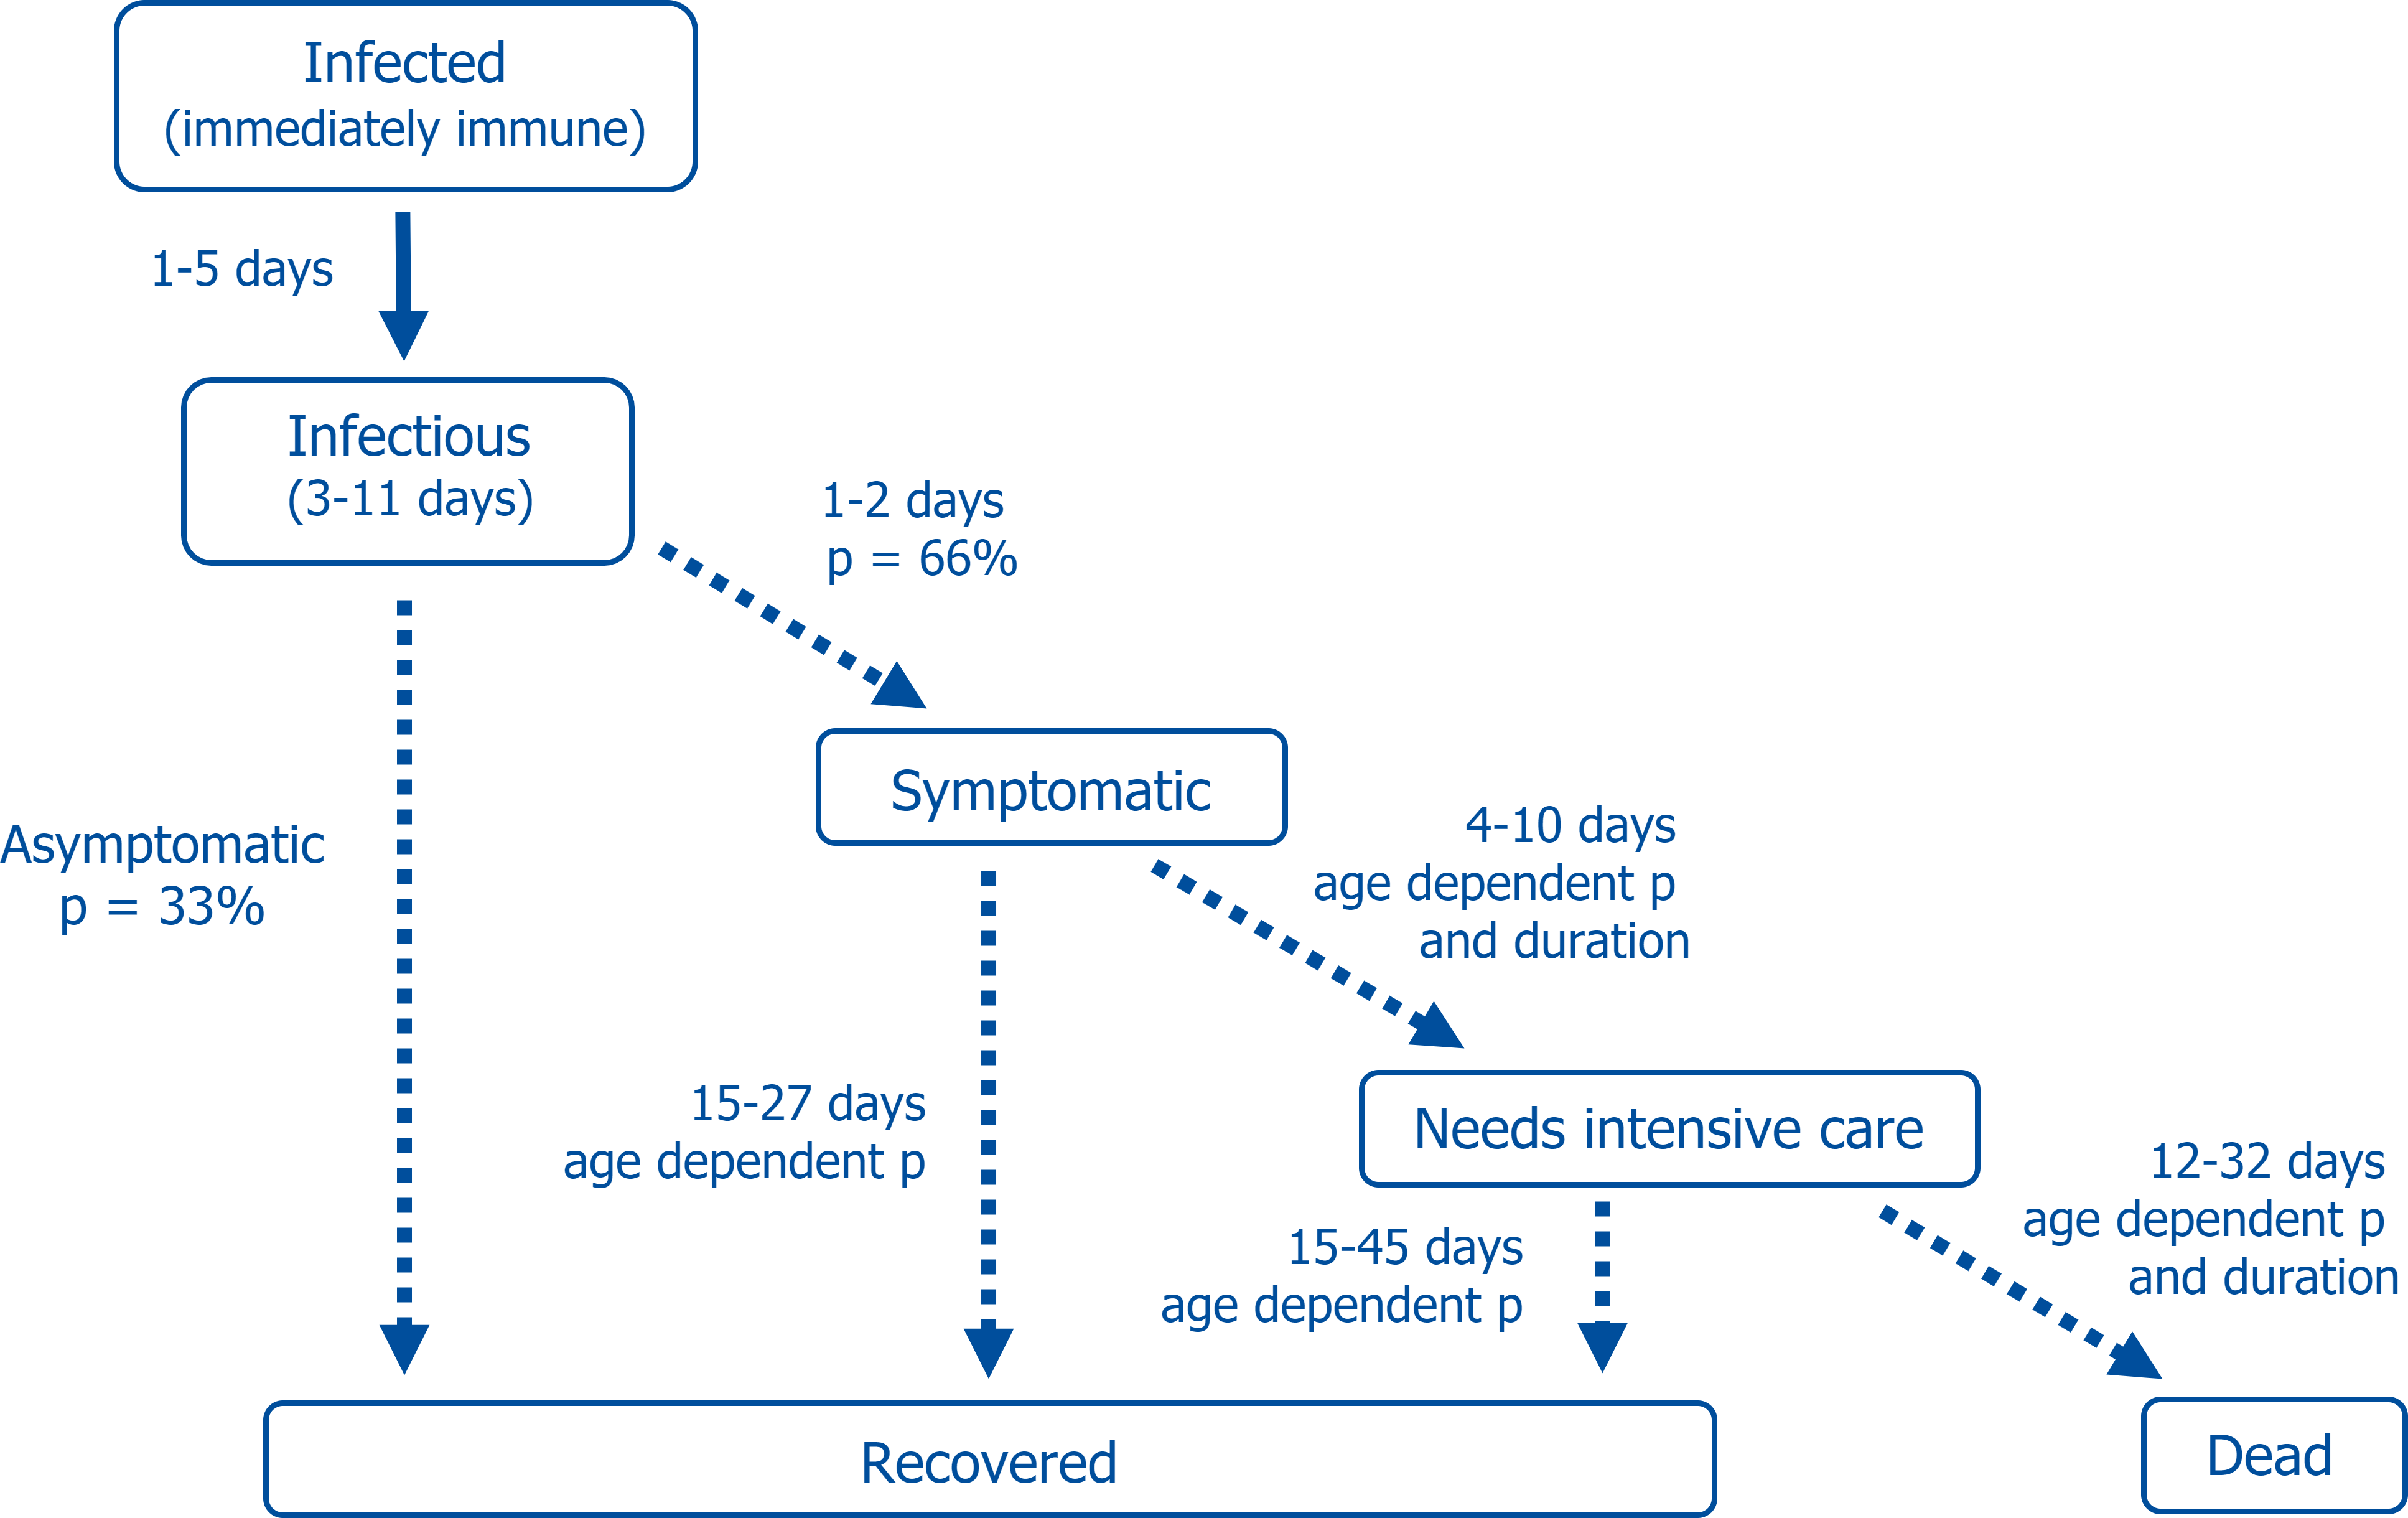
\includegraphics[width=\textwidth]{../figures/disease_progression.png}
    \caption{Course of Disease in the model}
    \label{fig:course_of_disease}
\end{figure}

First, infected individuals will become infectious after one to five days. About one third of people stays asymptomatic. The rest develops symptoms about one to two days after they become infectious. Modeling asymptomatic and pre-symptomatic cases is important because those people do not reduce their contacts or demand a test and can potentially infect many other people \citep{Donsimoni2020}.

A small share of symptomatic people will develop strong symptoms that require intensive care. The exact share and time span is age-dependent. An age-dependent share of intensive care unit (ICU) patients will die after spending up to 32 days in intensive care. Moreover, if the ICU capacity was reached, all patients who require intensive care but do not receive it die.

It would be easy to make the course of disease even more fine-grained. For example, we could model people who require hospitalization but not intensive care. So far we opted against that because only the ICU capacity might become a bottleneck in Germany.

We allow the progression of the disease to be stochastic in two ways: Firstly, state changes only occur with a certain probability (e.g. only a fraction of infected individuals develops symptoms). Secondly, the number of periods for which an individual remains in a state is drawn randomly. The parameters that govern these processes are taken from the literature. They can vary with the age of an individual.

Detailed information on the calibration of the disease parameters is available as part of our \href{https://sid-dev.readthedocs.io/en/latest/reference_guides/epi_params.html}{online documentation}.


\subsection{Testing} % (fold)
\label{sub:testing}

We support to model testing as consisting of three stages. Firstly, we model who demands
a test. Demand functions map from individual characteristics to a probability which is
the probability for this individual to demand a test. There can be multiple demand
functions where each function may describe a different channel. For example, individuals
who experience symptoms or have a risk contact may ask for a test. Or, the ministry of
education requires a negative test result from every teacher every second week. After
the probabilities for each individual and every demand model are computed, individuals
who demand a test as well as the channel is sampled.

The second stage is the allocation phase in which demand and supply for tests are
matched. The number of available tests can be inferred from official data and used to
model shortages in supply. When demand exceeds supply, some individuals might be given
preferred access to tests because of their own vulnerability or their potential to
become a super-spreader.

In the last and third phase, administered tests are processed. This step can become a
bottleneck in the testing process if there are not enough laboratories or necessary
resources available to evaluate all tests.

In our empirical estimation we use a very simplified testing model where the number of
tests to be distributed is calculated from estimates for the ratio of known to all
infections.\footnote{The Dunkelzifferradar project publishes daily estimates of the dark
figure of infections under \url{https://covid19.dunkelzifferradar.de/}} Using these
estimates as well as data on the test distribution over age groups by the
RKI\footnote{https://ars.rki.de/Content/COVID19/Main.aspx} we allocate tests firstly
among the symptomatic and then randomly allocate tests to newly infected to fit the
German test distribution.


% subsection testing (end)


\subsection{Seasonality}
\label{subsec:seasonality}

It is widely acknowledged that the transmission of SARS-CoV-2 is subject to seasonal
influences. Infectiousness is increased in winter when most contacts take place inside
and the immune system is weakened by low levels of vitamin D, dry air and large
temperature swings. For a detailed overview of possible drivers see
\cite{KronfeldSchor2021}.

We follow \cite{Kuehn2020} and \cite{Gavenciak2021} in modeling seasonality in the
transmission of SARS-CoV-2 as a multiplicative factor on infection probabilities. The
factor follows a sine curve that reaches its maximum at January first and its minimum
on June 30.

For simplicity we normalize the factor to reach one at its maximum. Thus the formula of
the seasonality factor is given by:

\begin{equation}
    s_k(t) = 1 + 0.5 \kappa_k  sin \left ( \pi  \left (\frac{1}{2} + \frac{t}{182.5}\right ) \right ) - 0.5 \kappa_k
\end{equation}

Where $\kappa_k$ is difference in the seasonality factor between peak infectiousness
and lowest infectiousness.

The subscript $k$ is needed because the strength of the seasonality effect differs
across contact types: Work, household and school contacts are likely to take place
inside even in summer. Thus they are only subject to seasonality due to factors that
influence the immune system. Other contacts (for example meeting friends and while doing
leisure activities) are mostly happening outside in the summer. Therefore, transmission
via those contacts should have a stronger seasonal pattern.

We calibrate $kappa_{strong}$ to 0.42 and $kappa_{weak}$ to 0.21. This is in line with
\cite{Gavenciak2021} and \cite{Kuehn2020}.


\subsection{Initial Conditions} % (fold)
\label{sub:initial_conditions}

Consider a situation where you want to start a simulation with the beginning set amidst
the pandemic. It means that several thousands of individuals should already have
recovered from the disease, be infectious, symptomatic or in intensive care at the start
of your simulation.
Additionally, the sample of infectious people who will determine the course of the
pandemic in the following periods is likely not representative of the whole population
because of differences in behavior (number of contacts, assortativeness), past policies
(school closures), etc..
The distribution of courses of diseases in the population at the begin of the simulation is
called initial conditions.

To come up with realistic initial conditions, we match reported infections from official
data to simulated individuals by available characteristics like age and geographic
information. The matching must be done for each day of a longer time frame like a month
to have individuals with possible health states. Then, health statuses evolve until the
begin of the simulation period without simulating infections by contacts.
We also correct reported infections for a reporting lag and scale them up to arrive
at the true number of infections.

% subsection initial_conditions (end)


% Additional Results

\subsection{Model Fit}
\label{subsec:fit_results}

This section compares simulated data from our model with empirical data from Germany. We
look at observed infections (overall as well as by age group and federal state), the
spread of the B.1.1.7 mutation, vaccinations\comment[id=K]{We fit vaccinations in the
population by construction. Maybe this should go to a different section?} and rapid test
demand.

% summary of the fit
Overall, our model achieves an excellent fit of the two waves of infections with few free
parameters (Figure~\ref{fig:aggregated_fit2}. As a result the effective replication
number is similar to that reported by the RKI (see Figure~\ref{fig:fit_r_effective}).
This excellent fit is also achieved for most age groups in Germany. The fit is also good
for many German federal states. Despite, the fact that the number of performed rapid
tests and their distribution in the population result endogenously inside our model we
fit the share of the population with at least a weekly rapid test very well and err on
the side of too few individuals that have ever done a rapid test.

% observed infections
Our fit of the infection rates in Germany between October 2020 and June 2021 is
excellent. The incidence in our model matches both the levels and the shape of the
reported incidence almost perfectly. When the prevalence of the virus is high and during
phases of exponential growth, the effect of random events on the incidence is large. That
is why it's important that we rely on 30 simulation runs with different seed sequences to
average over these random differences and have a stable mean.

\begin{figure}[ht]   % observed infections with single runs
  \centering
  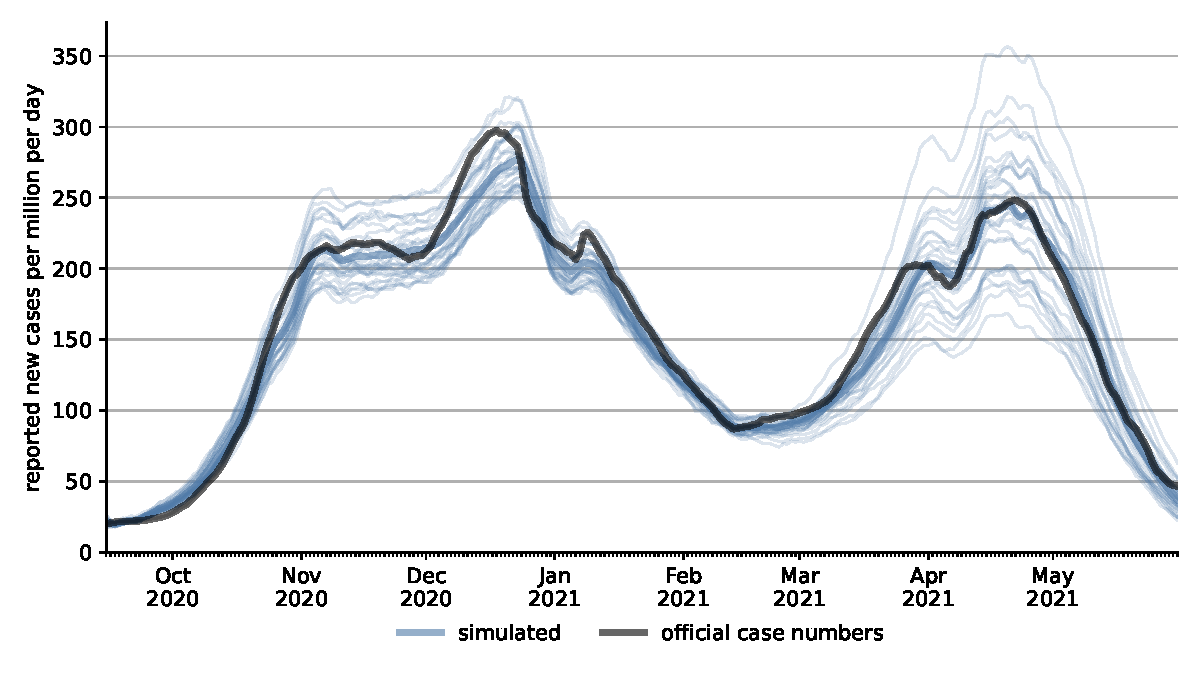
\includegraphics[width=\textwidth]{figures/results/figures/scenario_comparisons/combined_fit/full_new_known_case_with_single_runs}
  \caption{Fit Over the Full Simulation Time Frame with Single Simulation Runs}
  \floatfoot{\noindent \textit{Note:} The figure shows the daily incidence rate per
  million for the reported simulated infections rates. The mean infection rate is the
  thick blue line. Single simulation runs are plotted in lighter and thinner lines. The
  official case numbers as reported by the RKI are plotted in black. The fit is overall
  very good. The higher the mean incidence and the stronger the growth the more variance
  there is between simulation runs. We averaged over 30 simulation runs.}
  \label{fig:aggregated_fit2}
\end{figure}

% observed infections by age group
Zooming into the different age groups in Figure~\ref{fig:age_group_fit}, we can see that
our model is also able to reproduce the infection rates on this level. Differences
between the age groups allow us to identify the infection probabilities because different
age groups have contacts of different types (e.g. Mostly children go to school, the share
of workers is highest in the 35 to 59 age bracket etc.). There are very few points where
our simulated incidences and the empirical incidences do not
coincide:\comment[id=K]{@Janos: I think you can probably present this better...} Firstly,
the age group of 80 to 100 year olds due to the absence of nursing homes in our synthetic
population. Secondly, the increase in adolescents in April. We model the introduction of
rapid tests for students and do see an increase both in the observed infections and the
share of detected cases among students (see
Figure~\ref{fig:share_known_cases_by_age_group}). However, we follow \cite{Betsch2021}
that 82\% of all rapid tests are followed up with a PCR test. It is likely that that
share is higher for rapid tests that were done in schools. The last age group where our
fit does not fit the empirical curve very well is the group of 15 to 34 year olds. This
group has been touted to have a very active social life and it has often been suspected
that this age group also stayed more socially active during the pandemic. However, our
model does not include either effect because of very little data on both and hence it's
unsurprising that the actual case numbers in this group are consistently higher than our
simulated case numbers.\comment[id=K]{Does anyone have an idea why we do not match the
shape from Oct to Dec?}

\begin{figure}[ht]  % observed infections by age group
  \centering
  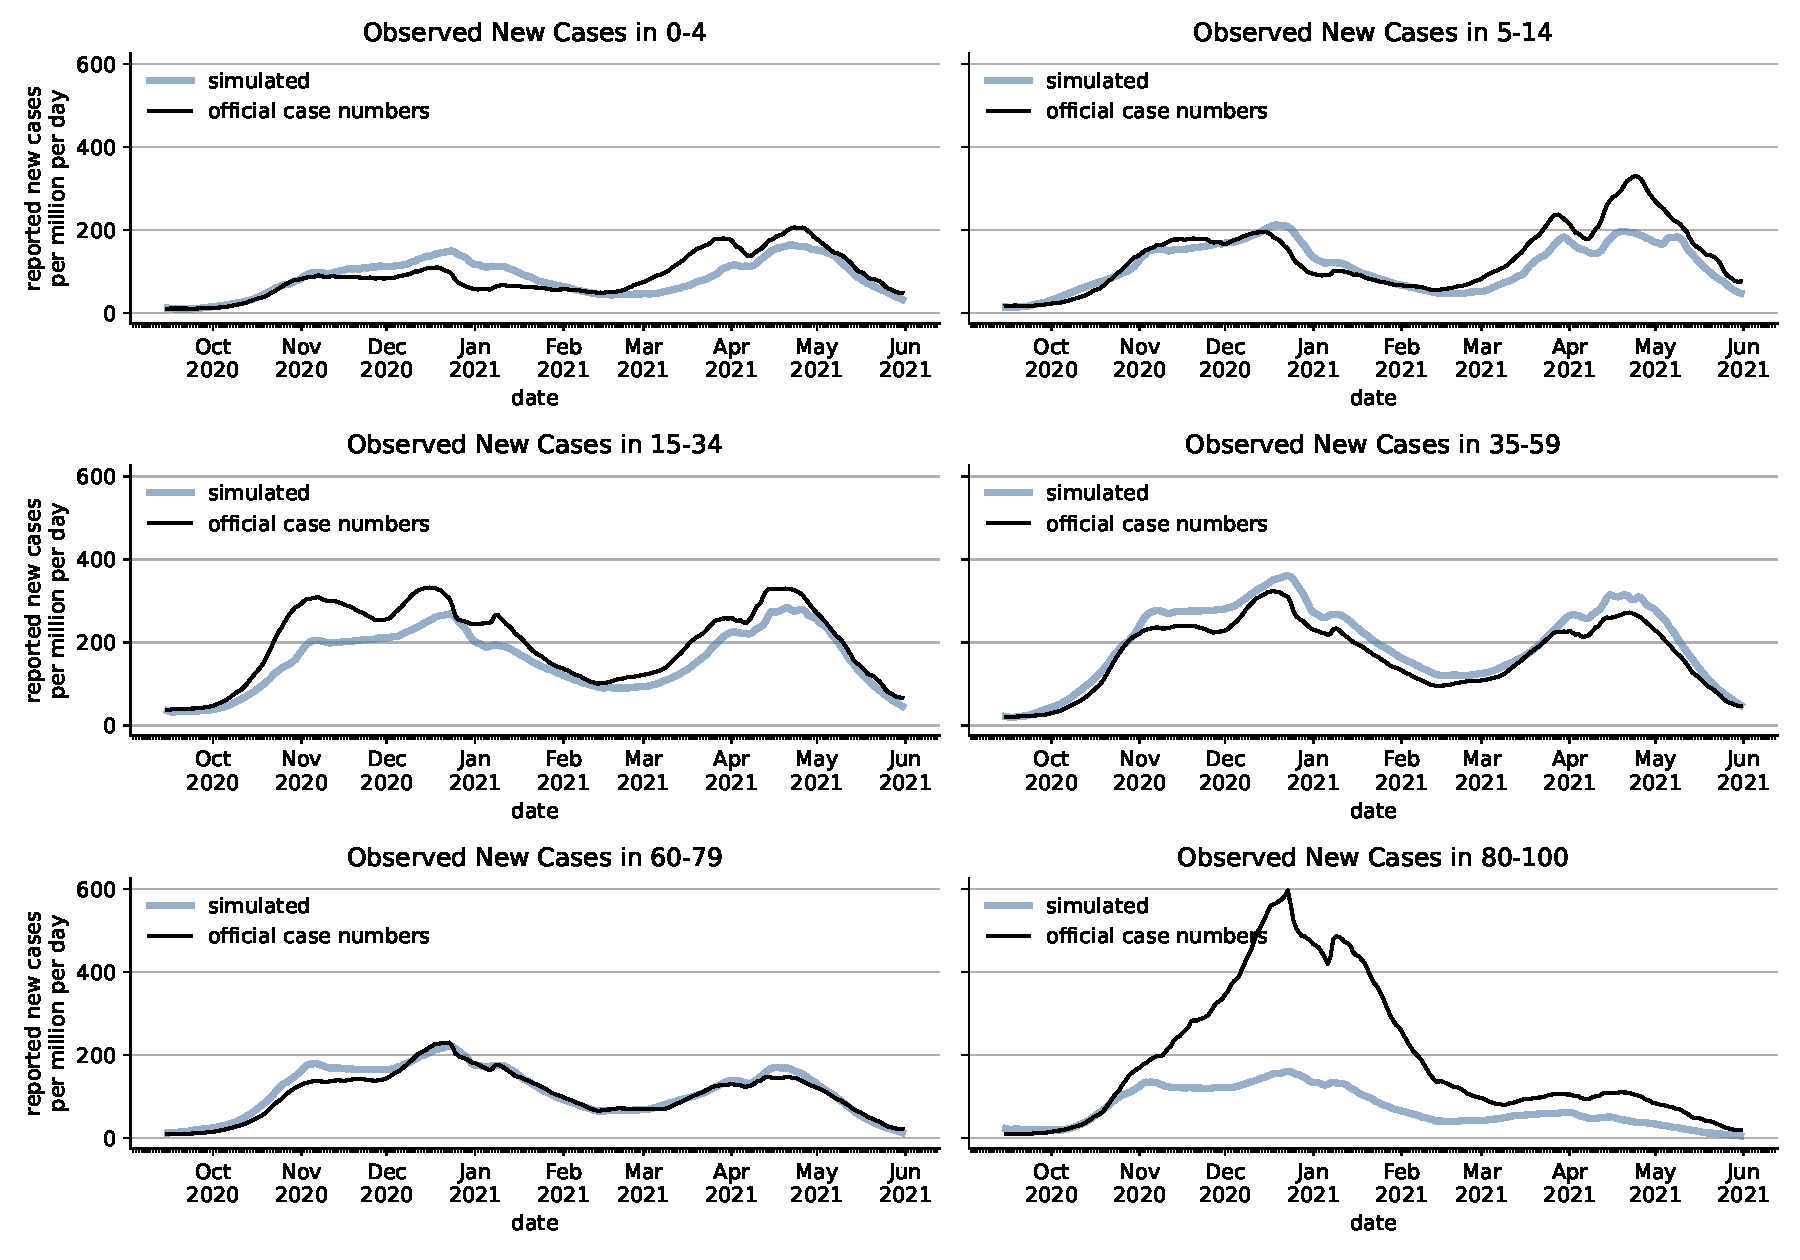
\includegraphics[width=\textwidth]{figures/results/figures/incidences_by_group/age_group_rki/full_combined_baseline_new_known_case}
  \caption{Simulated and Empirical Infections by Age Group}
  \floatfoot{\noindent \textit{Note:} The figure shows the weekly incidence rates per
  100,000 people for the reported versus the simulated infections rates for different age
  groups. The age group of individuals above 80 needs to be interpreted with caution
  because our synthetic population only includes private households, i.e. nursing homes
  are not represented in our model. They accounted for many cases and deaths in the
  winter of 2020 and many 80 to 100 year olds live in these facilities. However, the
  official data does not contain information on whether cases were nursing home
  inhabitants or not. We averaged over 30 simulation runs.}
  \label{fig:age_group_fit}
\end{figure}


\FloatBarrier

% observed infections by federal state
Our model fit is also very good for the different German federal states. This holds not
only for the large states such as North Rhine-Westphalia or Bavaria but also for many
smaller states such as Hessen or Rhineland-Palatinate. This shows that the inclusion of
school vacations and relying on work reductions by \cite{Google2021} combined with the
assortativity of contacts on the county level is sufficient to represent many local
differences.  %
However, admittedly, there are several patterns that our model does not reproduce - for
example because we do not have cross-border travel nor population density. This explains
why our model produces too many infections for federal states such as Schleswig-Holstein
and why it predicts too few infections for states, such as Saxony, bordering high
incidence countries.\comment[id=K]{The Czech Republic had very high numbers in October
(max > 800) but they fell during Nov to 220 and then climbed again to 800 by Jan 12th so
that might be only part of the answer why Saxony had such high numbers.}
However, these missing features are irrelevant for our main conclusions.


\begin{figure}[ht]   % observed infections by federal state
  \centering
  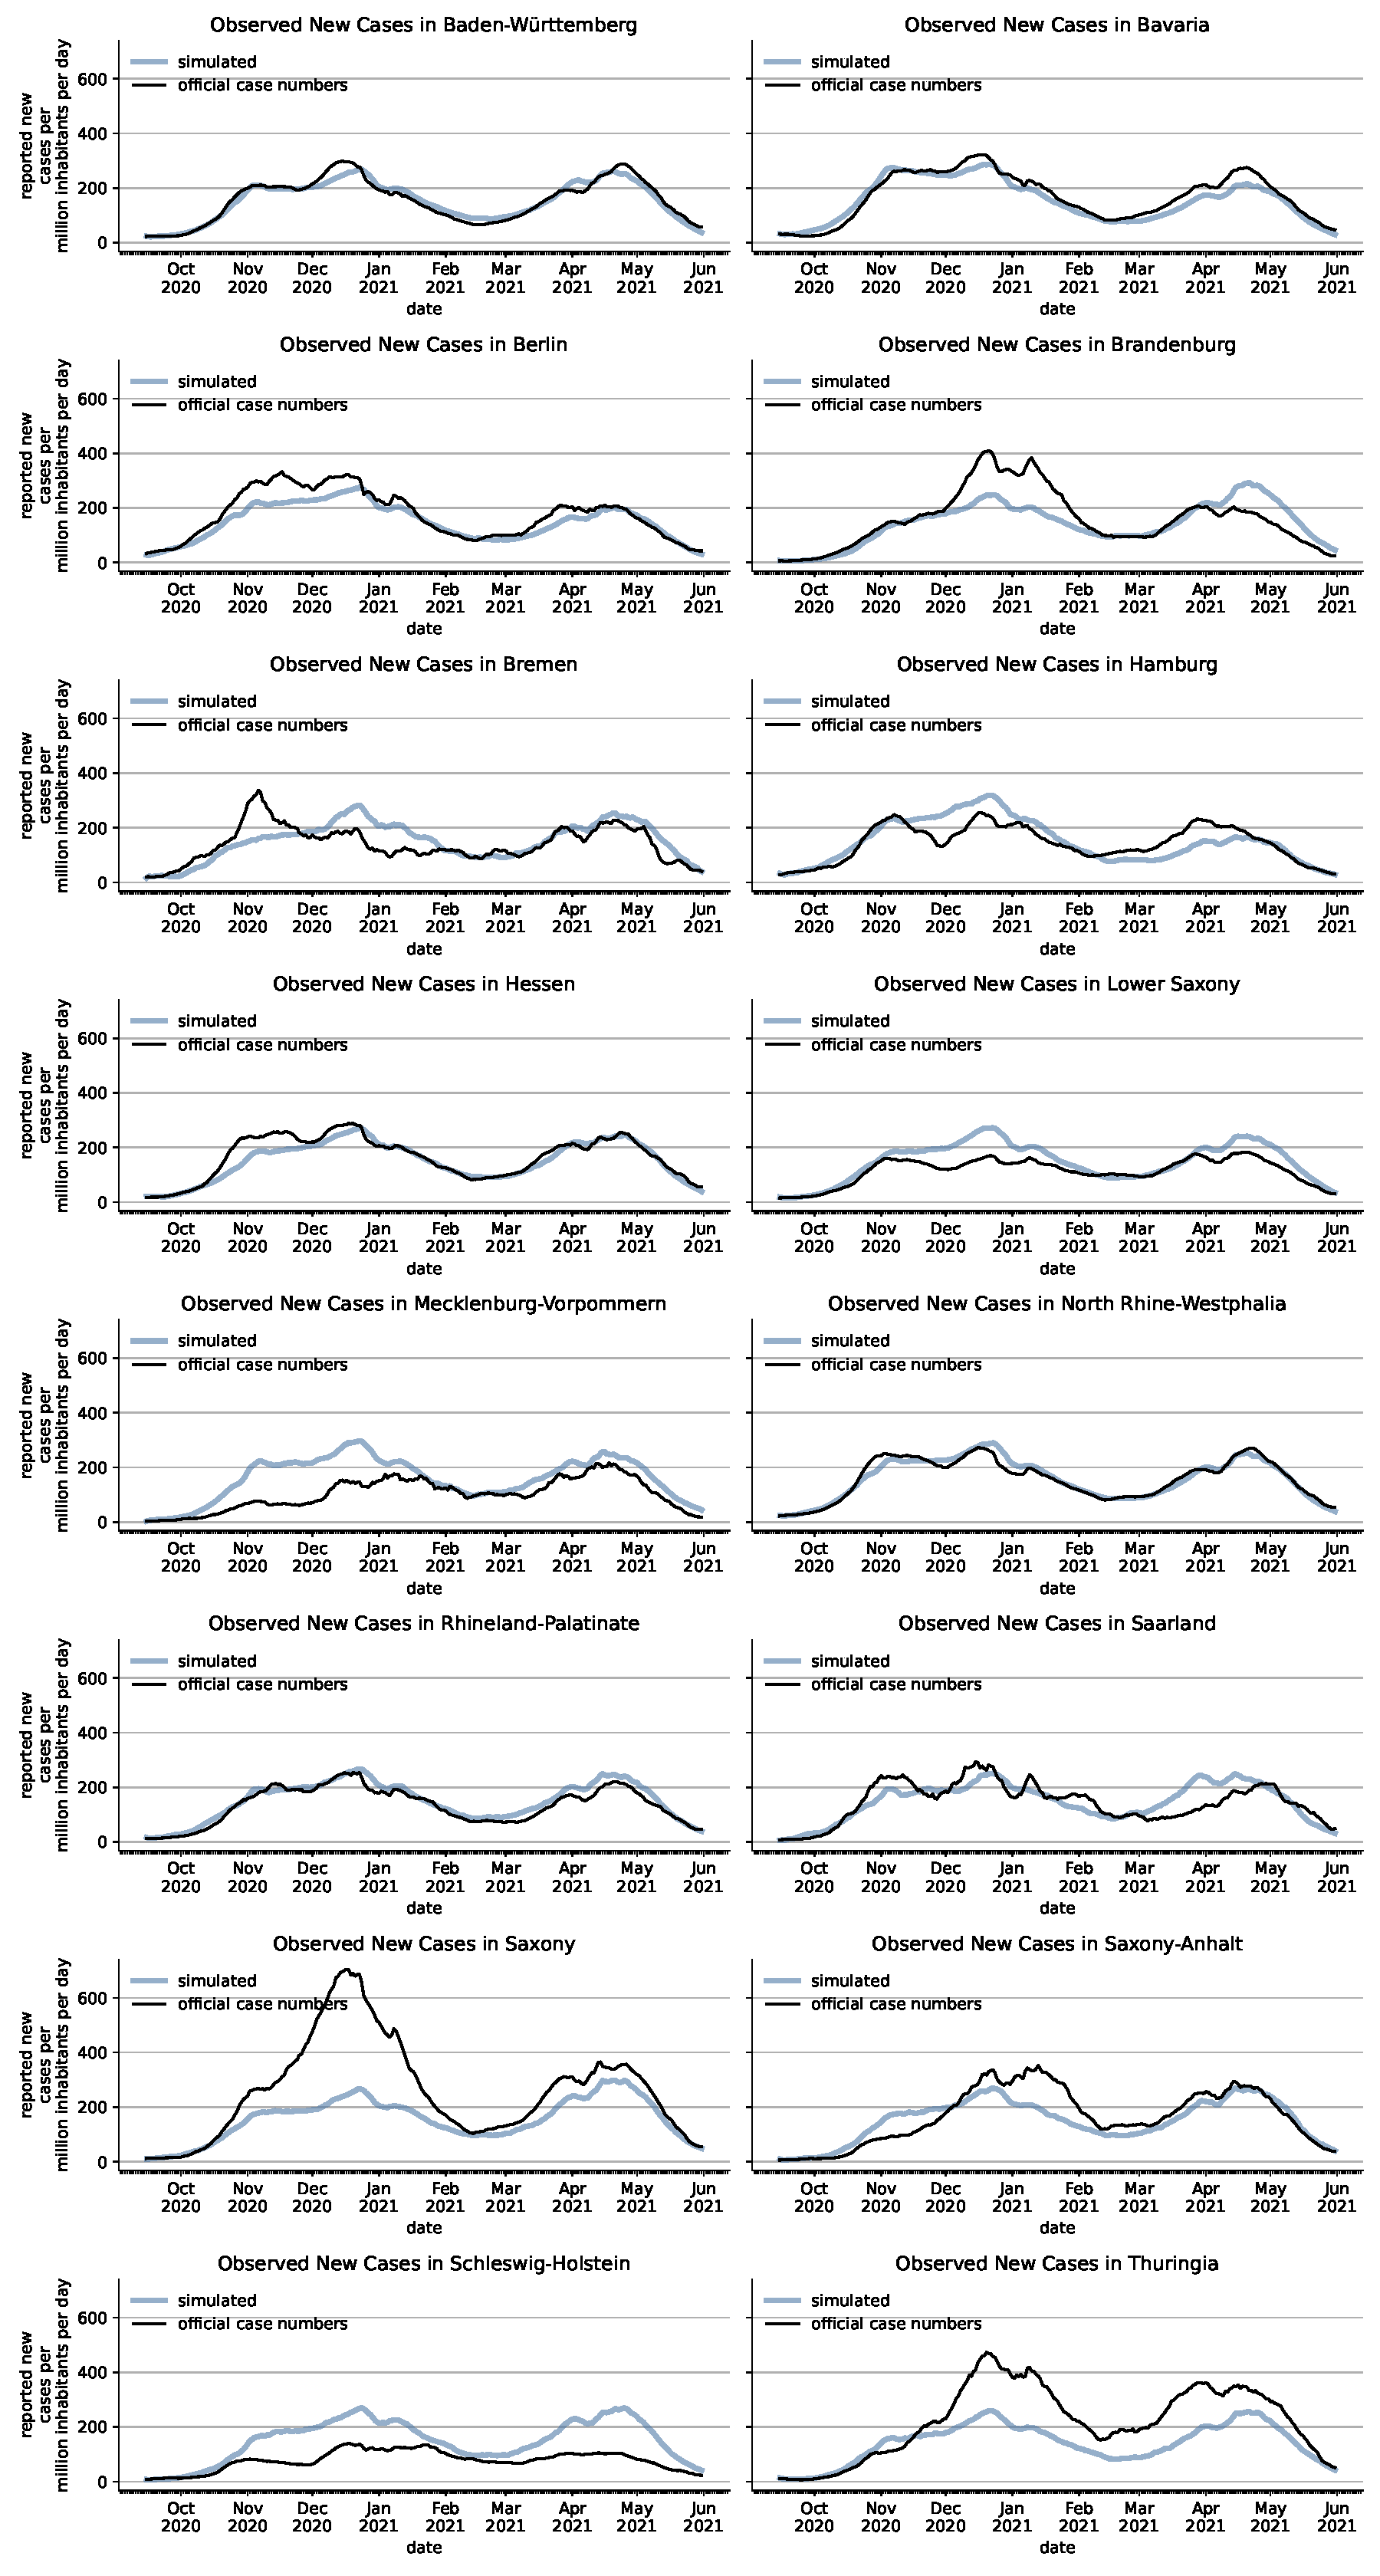
\includegraphics[height=0.95\textheight]{figures/results/figures/incidences_by_group/state/full_combined_baseline_new_known_case}
  \caption{Simulated and Empirical Infections by Federal State}
  \floatfoot{\noindent \textit{Note:} The figure shows the weekly incidence rates per
  100,000 people for the reported versus the simulated infections rates for different
  federal states. We averaged over 30 simulation runs.}
  \label{fig:state_fit}
\end{figure}

\FloatBarrier

Our fit of the effective replication number $R_t$ closely follows the values reported by
the RKI even though we calculate $R_t$ on all infected individuals not just the detected
cases. This explains why the $R_t$ in our simulations is higher during phases where the
share of detected cases falls such as in the fall of 2020 (see
Figure~\ref{fig:share_known_cases_data}) where the RKI underestimated the effective
replication number due to observing a lower share of cases and is lower than the $R_t$
reported by the RKI in spring where the share of known cases increased due to increased
rapid testing.

\begin{figure}[ht]   % R effective
  \centering
  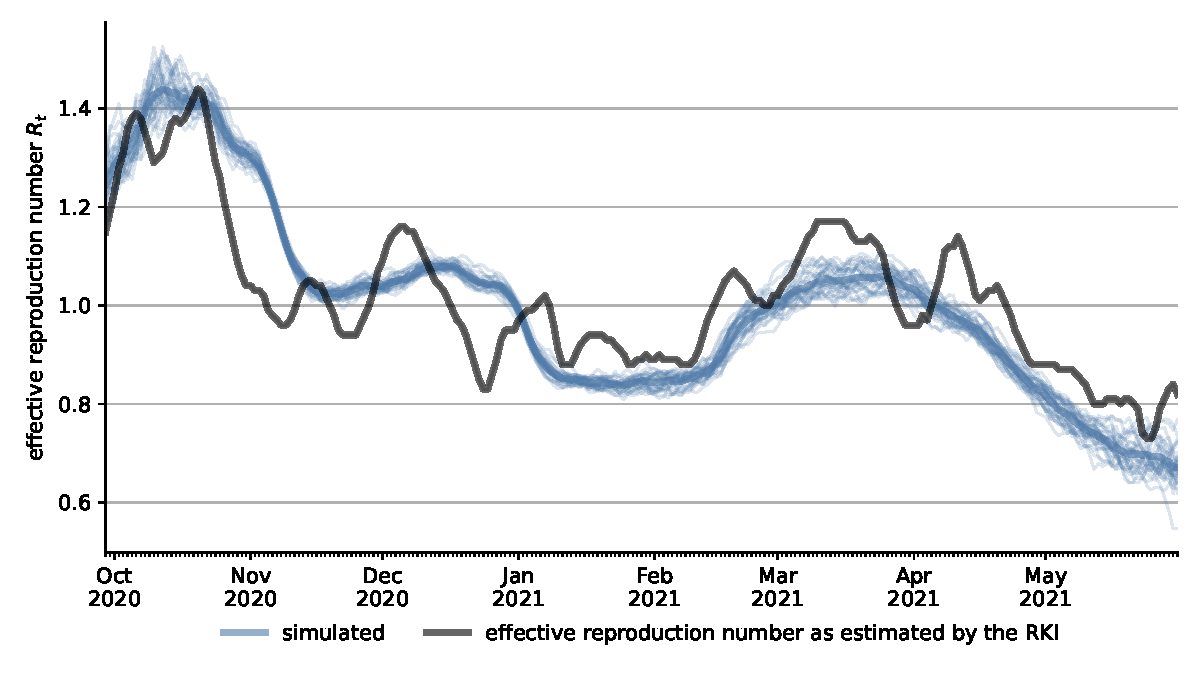
\includegraphics[width=\textwidth]{figures/results/figures/scenario_comparisons/combined_fit/full_r_effective_with_single_runs}
  \caption{Effective Replication Number $R_t$ in the Model and as Reported by the
  Robert-Koch-Institute}
  \floatfoot{\noindent \textit{Note:} The figure shows the effective replication number
  ($R_t$) as reported by the RKI and as calculated in our model. The $R_t$ gives the
  average number of new infections caused by one infected individual. The $R_t$ in our
  model broadly follows the $R_t$ reported by the RKI. Two trends stand out. Firstly, the
  RKI's $R_t$ drops faster in November. This could be due to a change in the testing
  policy that focused tests on the elderly when the second wave hit Germany and led to a
  decline in the overall share of detected cases. The second difference is from mid
  February to mid March where the RKI's reported $R_t$ increased more rapidly than that
  in our model. Here the opposite effect can be expected. During this time rapid tests
  increased strongly leading to more cases being detected. In the short term this leads
  an $R_t$ estimation that is based on detected cases to overestimate the replication
  number.}
  \label{fig:fit_r_effective}
\end{figure}

% B.1.1.7
We fit the proliferation of the B.1.1.7 variant quite exactly despite only introducing a
few cases in January as can be seen in Figure~\ref{fig:fit_share_b117}. Since we only
model B.1.1.7 and do not include other variants B.1.1.7 reaches a share of nearly 100\%
by May while the true rate plateaued at 90\% and B.1.1.7 was then replaced by B.1.617.2
as the dominant variant in June. However, B.1.1.7 still made up over 90\% of all cases in
Germany at the end of our simulation period.

\begin{figure}[ht]   % Share B.1.1.7
  \centering
  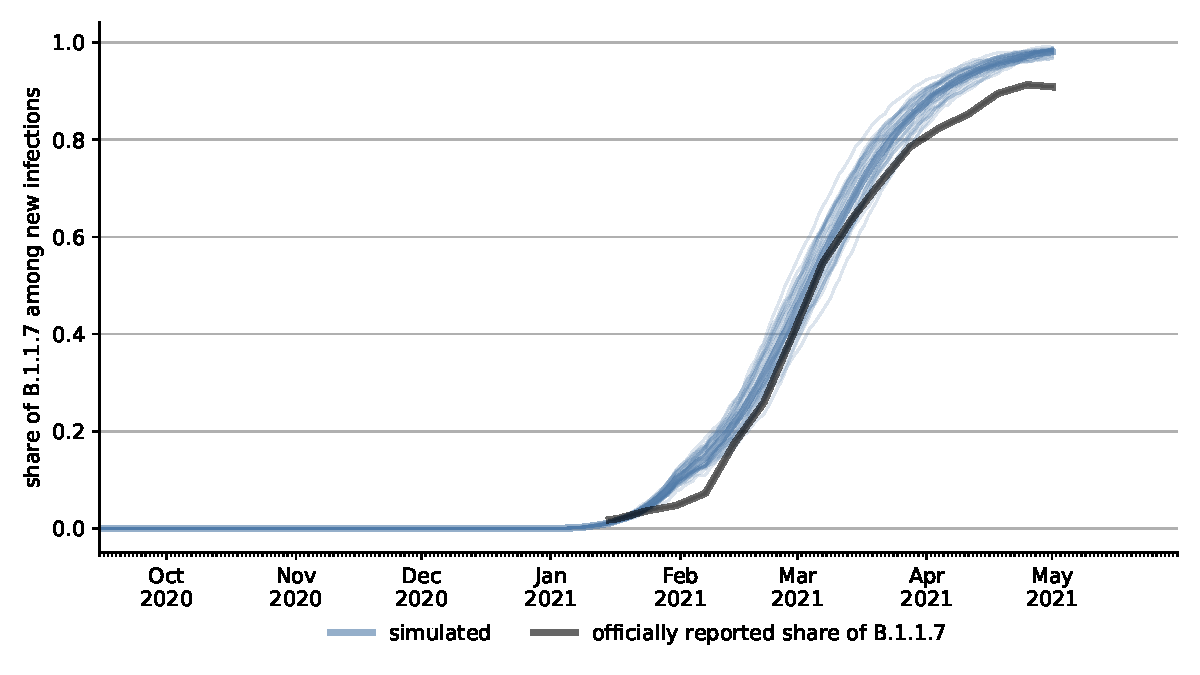
\includegraphics[width=\textwidth]{figures/results/figures/scenario_comparisons/combined_fit/full_share_b117_with_single_runs}
  \caption{Share of B.1.1.7 in the Model and as Reported by the Robert-Koch-Institute}
  \floatfoot{\noindent \textit{Note:} The figure shows the share of B.1.1.7 as
  reported by the RKI and as calculated in our model. We only introduce a few cases over
  the cause of January. From then B.1.1.7 takes over endogenously through its increased
  infectiousness. We model no other features of B.1.1.7. At most we introduce 0.75 cases per 100,000 inhabitants.}
  \label{fig:fit_share_b117}
\end{figure}

% vaccinations

The fit of the share of vaccinated individuals can be seen in
Figure~\ref{fig:fit_vaccinations}. In Germany, vaccines were rolled according to four
priority groups. The first vaccines were mostly reserved for nursing homes and some
selected professions such as first responders. Since we do not have nursing home
inhabitants in our model, we subtract the first percent of vaccinations which is
equivalent to the share of Germans living in nursing homes. Afterwards, the share of
vaccinated individuals in the population follows the German increase quite exactly. We
took great care to model the prioritization of older individuals and professions that
cannot reduce physical contact easily such as teachers or medical staff (see
Section~\ref{subsec:synthetic_population}. How the share of vaccinated individuals
develops by age group can be seen in Figure~\ref{fig:vaccinations_by_age_group}.

\begin{figure}[ht]   % fit of vaccinations
  \centering
  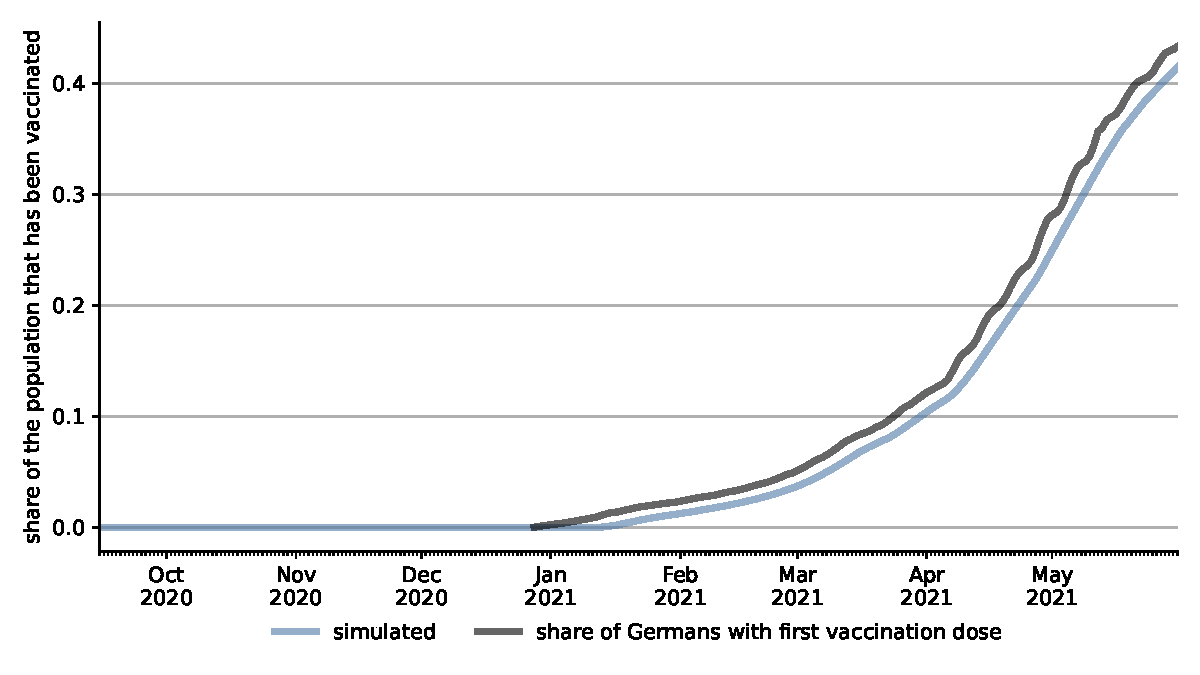
\includegraphics[width=\textwidth]{figures/results/figures/scenario_comparisons/combined_fit/full_ever_vaccinated}
  \caption{Share of Vaccinated Individuals}
  \floatfoot{\noindent \textit{Note:} The figure shows the rate of individuals that are
  vaccinated in our synthetic population versus in the general German population. Note
  that we excluded the vaccinations that were given to nursing homes, approximately the
  first percent of the German population that were vaccinated. Overall, our model covers
  a time frame that goes from zero vaccinated individuals to a state where over 40\% of
  the population are vaccinated. Our vaccinations work imperfectly but we do not model
  different vaccines nor do we distinguish between first and second shot.}
  \label{fig:fit_vaccinations}
\end{figure}

% rapid test demand
The most difficult moment to match in our model is the rapid test demand. Since we have
five different channels through which individuals demand rapid tests and many of the
demand curves are at least partially calibrated through survey data. It is therefore very
reassuring that we fit the share of individuals that do weekly rapid tests almost
perfectly. For the share of individuals that have ever done a rapid test our model is
conservative. There are two reasons for this: Firstly, we only introduce rapid tests in
2021. This is due to the small number of rapid tests in 2020 as well as a lack of data on
the number of random tests and who received them. Secondly, there is no randomness in an
individual's rapid test demand. This reduces the randomness in our model at the cost of
having less individuals that only occasionally test themselves. \comment[id=K]{Write that
this makes us underestimate the effect of random tests?} However,
Section~\ref{subsec:model_validation} shows that our results are very robust to changes
in the exact shares of individuals demanding rapid tests.

\begin{figure}[ht]     % rapid test demand
    \centering
    \caption{Share of Individuals With Rapid Tests}
    \label{fig:share_ever_rapid_test2}
    \begin{subfigure}{.55\textwidth}
        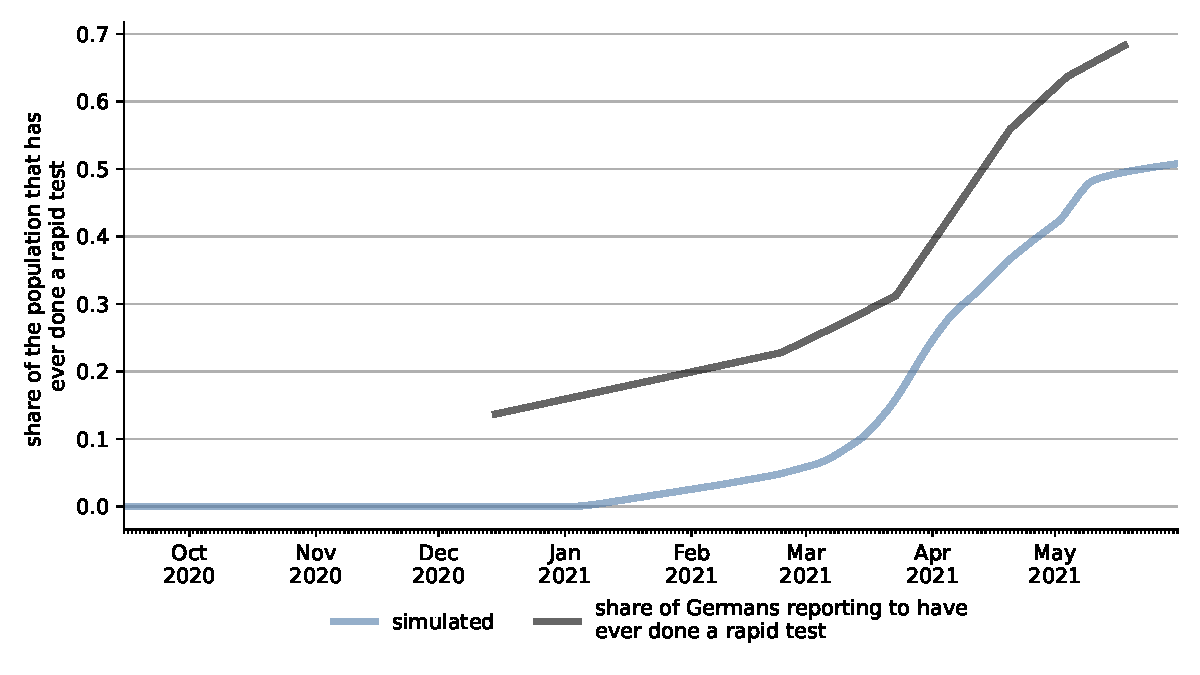
\includegraphics[width=0.9 \textwidth]{figures/results/figures/scenario_comparisons/combined_fit/full_share_ever_rapid_test}
        \caption{Share of Individuals That Have Ever Done a Rapid Test}
    \end{subfigure}%
    \begin{subfigure}{.55\textwidth}
        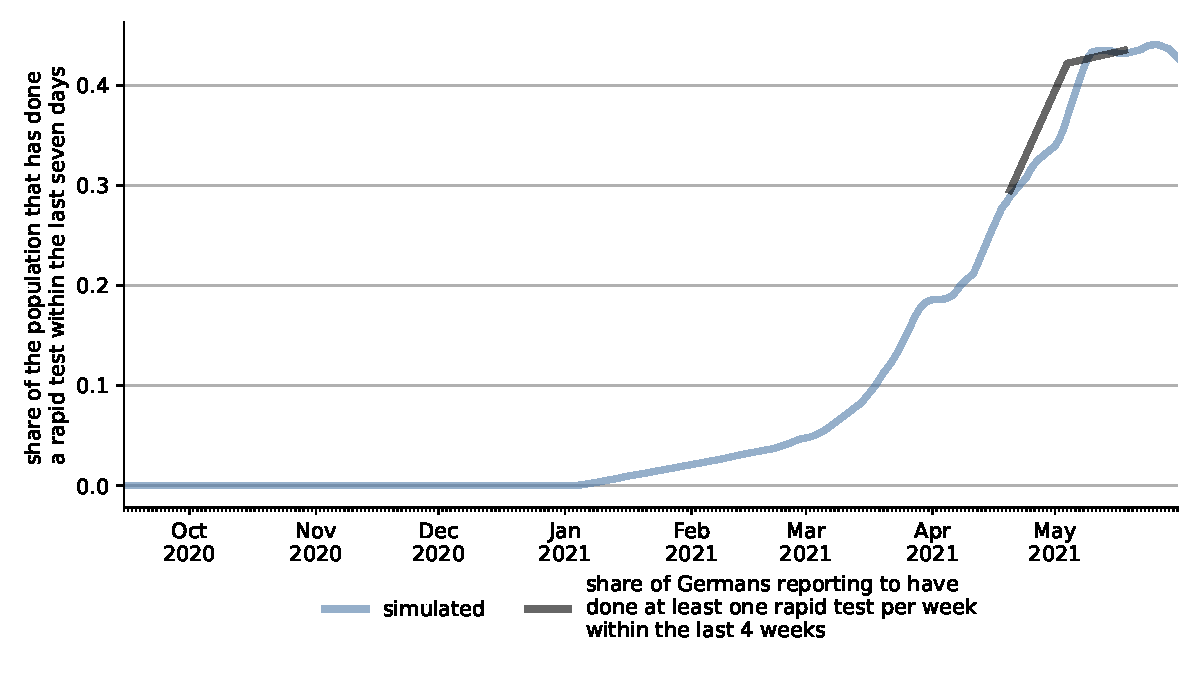
\includegraphics[width=0.9 \textwidth]{figures/results/figures/scenario_comparisons/combined_fit/full_share_rapid_test_in_last_week}
        \caption{Share of Individuals Having Done a Rapid Test in the Last Week}
    \end{subfigure}
    \label{fig:share_rapid_test_last_week2}
    \floatfoot{\noindent \textit{Note:} The figure compares the share of individuals who
        have ever done a rapid test or done a rapid test within the last week in our
        simulations to the shares reported in the
        \href{https://projekte.uni-erfurt.de/cosmo2020/web/topic/wissen-verhalten/80-schnelltests/}{COVID-19
        Snapshot Monitoring Survey}. The left panel compares the share of individuals who
        have ever done a rapid test. The right panel compares the share of individuals
        who have done a rapid test within the last seven days in our simulation compared
        to the share reporting to have done at least weekly rapid tests in the last four
        weeks in the COSMO survey. Overall our calibration of rapid tests are slightly
        conservative. The overall share is below that in the study. We fit the share of
        weekly tests quite exactly. However, the study only covers adults while our share
        also includes children who are tested very regularly when attending school.}
\end{figure}



\FloatBarrier



\subsection{Model Validation}
\label{subsec:model_validation}

Achieving a good in-sample fit does not necessarily guarantee that our model will also
be able to make out of sample predictions. For example, it could be that the results
are very sensitive to the exact number of vaccinations, the work mobility multiplier
or the number of rapid tests that are performed -- all of which are things that cannot
be exactly known ex-ante.

In this section we compare simulated infections that use all available data with
out of sample predictions that only use data that was available at March 1 2021.

For the out of sample predictions we predict the number of vaccinations between March
and June with a simple linear regression model that was fitted on vaccine data from
February. The work mobility multiplier is predicted to be constant at a value of
0.75, which is an approximate average of the second half of February.

The area that is frought with the most uncerainty are the introduction of rapid test,
because it comprises both, supply and demand factors. Moreover, accurately predicting
the number of rapid tests ist expected to be important because rapid tests play a large
role for the transmission dynamic.



\begin{figure}[ht] % Robustness Check
  \centering
  \begin{subfigure}[b]{.49\textwidth}
    \centering
    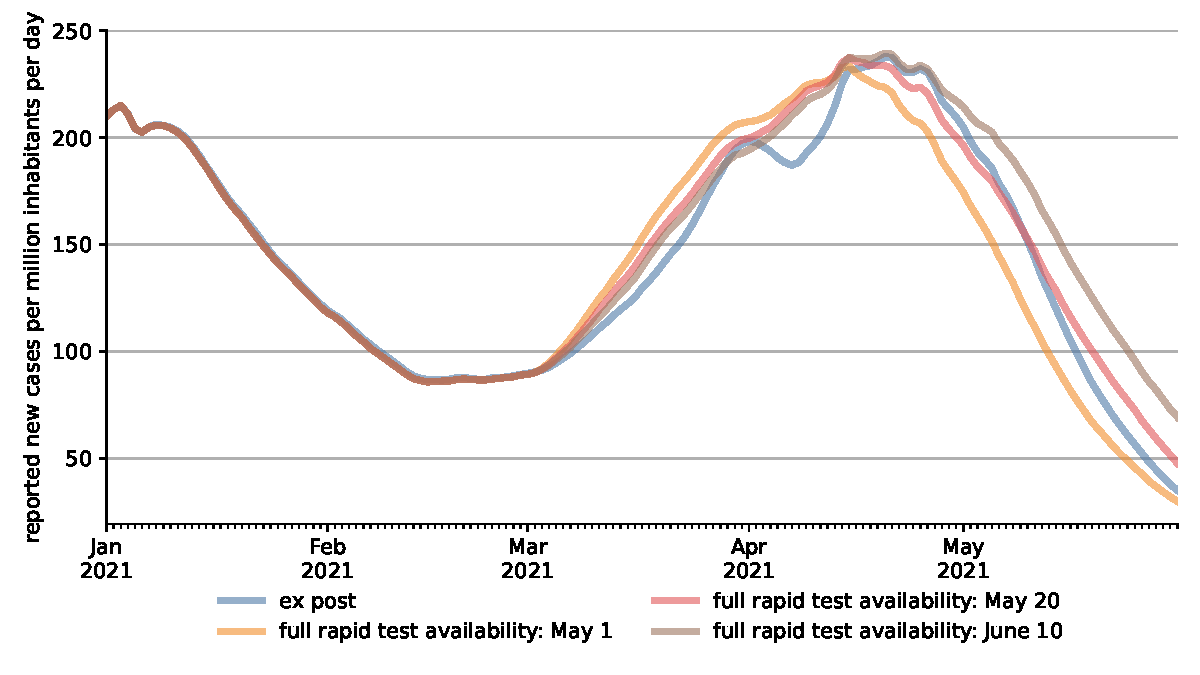
\includegraphics[width=0.9 \textwidth]{figures/results/figures/scenario_comparisons/robustness_check/full_new_known_case}
    \caption{Reported Cases}
    \label{fig:robustness_check_new_known_case}
  \end{subfigure}%
  \hfill
  \begin{subfigure}[b]{.49\textwidth}
    \centering
    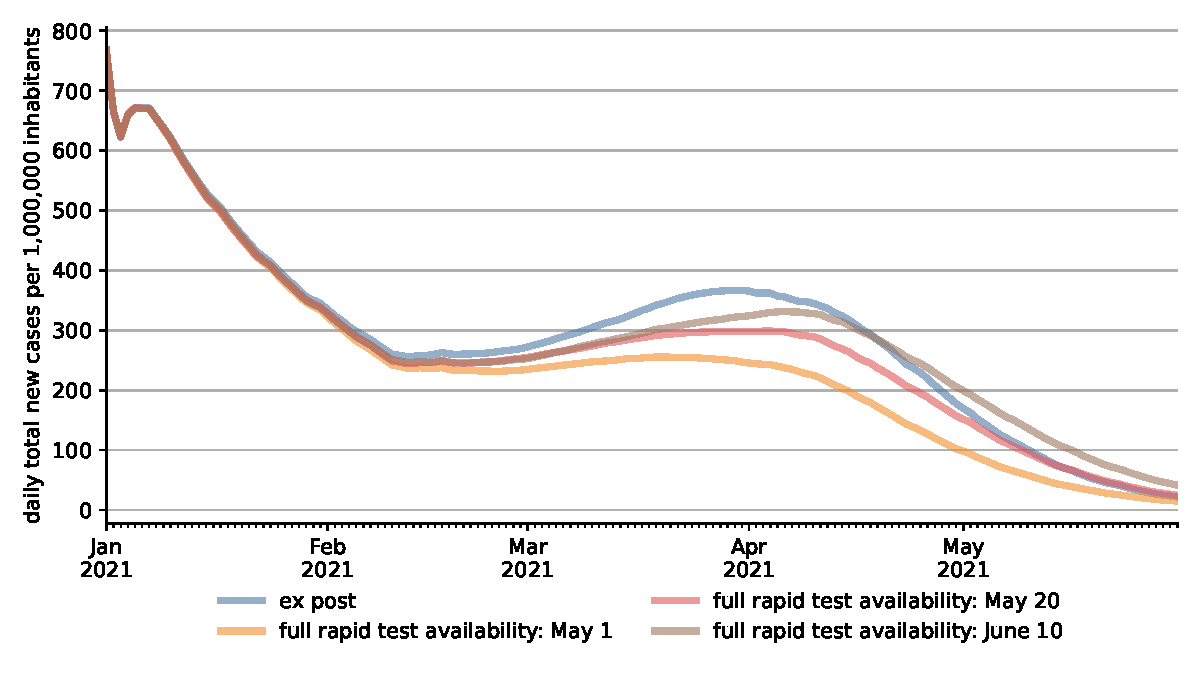
\includegraphics[width=0.9 \textwidth]{figures/results/figures/scenario_comparisons/robustness_check/full_newly_infected}
    \caption{Total Cases}
    \label{fig:robustness_check_newly_infected}
  \end{subfigure}
  \caption{Out of sample prediction for reported and total cases from March to June
    2021. The ex-post scenario is an in-sample prediction that uses all available
    information and is very close to actual case numbers. For the other scenarios data
    on vaccinations, work mobility and rapid tests that became available after March 1
    have been replaced by prediction models that are calibrated with data from February.
    Moreover, they do not model a lower number of detected cases over the easter
    holidays. The different scenarios make different assumptions on the date at which
    full availability of rapid tests is reached. While the out of sample predictions
    differ substantially for the exact case numbers at the beginning of June (between
    20 and 70 cases per million), they can all reproduce the decline in case numbers
    that is jointly driven by seasonality, large scale rapid tests and vaccinations.
  }
  \label{fig:robustness_check_detailed}
  \floatfoot{\noindent \textit{Note:} \textcolor{red}{To be written}}
\end{figure}

 \comment[id=K]{@Janos: Please add caption and description for the robustness check.}


\subsection{Robustness to assumptions about rapid test sensitivity}
\label{subsec:robustness_rapid_test_sensitivity}

\Copy{r.1.b-appendix}{
    Our main results are based on rapid test sensitivities read from clinical trials. Recent studies showing that the actual sensitivity of rapid tests may be lower than that \citep[e.g.,][]{Scheiblauer2021}.

    This section shows that our results are robust to making less favorable assumptions
    on rapid test sensitivity. We proceed by describing several possible ways of
    calibrating rapid test sensitivity profiles based on recent studies. Since none of
    these methods is inherently better than the others, we make simulations with two
    sensitivity profiles: The average over all methods and the lower envelope over all
    methods using recent studies.

    Both profiles imply lower sensitivities of rapid tests than used in our main
    results. This is especially true during the later stage of an infection. However,
    the main results stay very robust. The original result was that rapid tests,
    seasonality and vaccinations are responsible for 42\%, 43\% and 16\%, respectively.
    With the average profile, the effect of rapid tests decreases to 41 \%. With the
    lower envelope profile, which is an extremely unfavorable assumption, it becomes
    38\%.

    % what do we need
    The effect of rapid tests on infection dynamics strongly depends on \emph{when} an
    infection is detected. Earlier detection means that it is more likely that the
    infection has not yet been discovered for a different reason (e.g. due to the onset
    of symptoms) and that the infected person can be isolated before spreading the
    disease to others.

    The sensitivity of rapid tests depends on the viral load in the respiratory tract.
    It is low at the beginning of an infection (especially before the onset of
    infectiousness), high in the first few days of infectiousness and then gradually
    decreasing towards the end of infectiousness.

    We thus need to calibrate a profile of rapid test sensitivities based on the number
    of days until or since the onset of infectiousness.

    % what is available -> two step mapping
    Unfortunately, such sensitivity profiles are not usually reported in studies. We
    thus need to create them by combining two types of studies: 1. Studies that report
    the viral load in terms of threshold cycle ($Ct$) values determined by PCR test
    \citep[e.g.][]{Cosentino2022,Ong2021,Bonnet2022,Jang2021,Zuin2021}. 2. Studies that
    report the sensitivity of rapid tests for different $Ct$ values
    \citep[e.g.][]{Scheiblauer2021,Bruemmer2021}.

    % what options do we have to configure the mappings
    It is natural to assume that the evolution of $Ct$ values over time as well as the
    effect of $Ct$ values on rapid test sensitivity are continuous functions. However,
    the results of the available studies are usually reported in a discretized way. This
    leads to multiple ways of calculating the sensitivity profiles. Some try to recover
    the underlying continuous functions using interpolation or regression, others simply
    use the discretized values.

    % Describe CT value formula vs. bin averages
    For the calibration of $Ct$ values over time we can either use discretized values
    for several time bins from \cite{Ong2021} and \cite{Jang2021}. Alternatively, we can
    use linearized formulas for calculating sensitivities over time \cite{Cosentino2022}
    and complement it with interpolations of data points from \cite{Jang2021} in the
    pre-infectious stage. Throughout we assume that the $Ct$ values of individuals who
    eventually develop symptoms and those who do not follow the same trajectory. This is
    in line with results by \cite{Zuin2021} and recent evidence that rapid tests excel
    at discovering asymptomatic cases \cite{Rosella2022}.

    % Describe sensitivity lookupd vs. interpolation
    For the mapping of $Ct$ values to rapid test sensitivities, again we have two
    options. First, we can simply look up the discretized values for the three $Ct$ bins
    provided in \cite{Scheiblauer2021} (below 20, 25 to 30 and above 35). Secondly, we
    can use linear regression to estimate a continous mapping for the relationship by
    assuming that the $Ct$ values of each bin are achieved exactly at the bin midpoints
    and that the relationship is linear.

    % Properties of the different methods
    In general, using discretized values can lead to an underestimation of peak
    sensitivities and an overestimation of very low sensitivities. This is because
    discretization is essentially a smoothing device. On the other hand, it has the
    advantage of simply working with published results, without introducing any tuning
    parameters or other assumptions.

    % resulting profiles.
    \begin{figure}
        \centering
        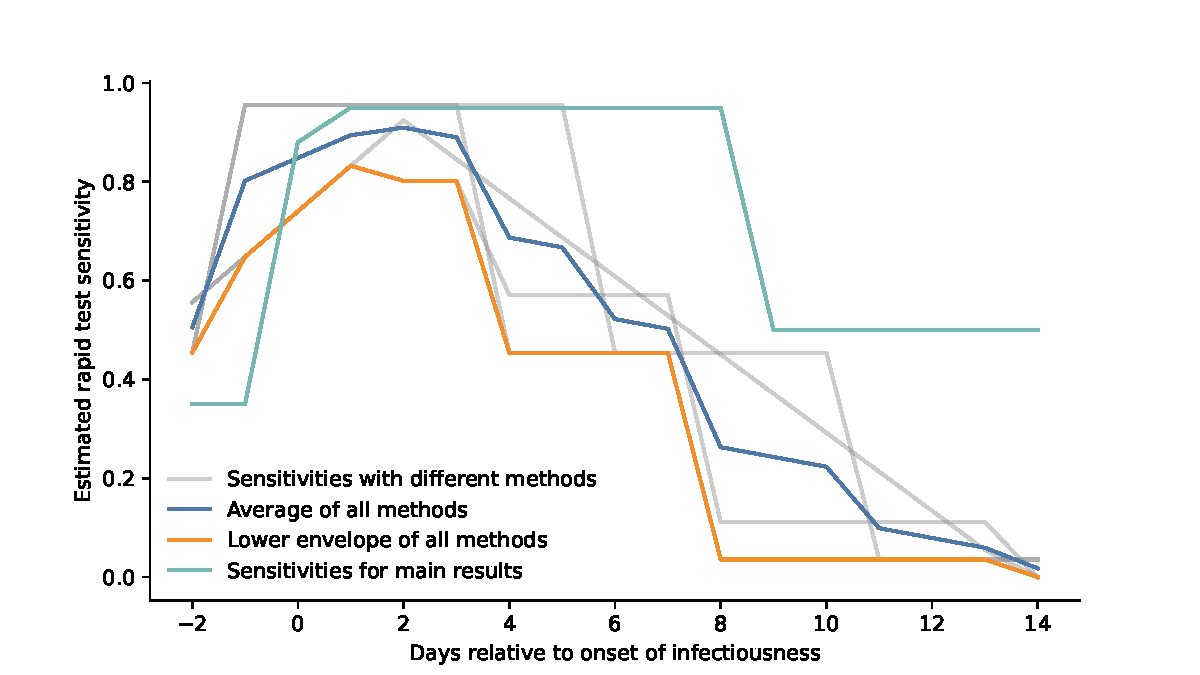
\includegraphics[width=0.9\textwidth]{figures/results/figures/data/testing/sensitivity_params_with_different_methods}
        \caption{Rapid test sensitivity profiles}
        \floatfoot{\noindent \textit{Note:} The figure shows estimated sensitivities of
            rapid tests over the course of an infection. The x-axis shows days relative
            to the onset of infectiousness. The y-axis shows the estimated rapid test
            sensitivities. The grey lines are the raw sensitivity estimates obtained
            with different methods of dealing with discretized data. The blue line shows
            their average and the yellow line their lower envelope. The turquoise line
            are the test sensitivities used for the main results of the paper.}
        \label{fig:sensitivity_assumptions}
    \end{figure}

    \FloatBarrier

    Figure \ref{fig:sensitivity_assumptions} shows that the updated sensitivity
    estimates are lower than the ones used for our original results, especially towards
    the end of an infection. However, the main results barely change. This is due to the
    fact that the differences are largest towards the later stage of an
    infection. Uncovering an infection that was previously undetected at that stage does
    not have a large effect on infection dynamics.

    \begin{figure}
        \centering

        \begin{subfigure}[b]{0.475\textwidth}
            \centering
            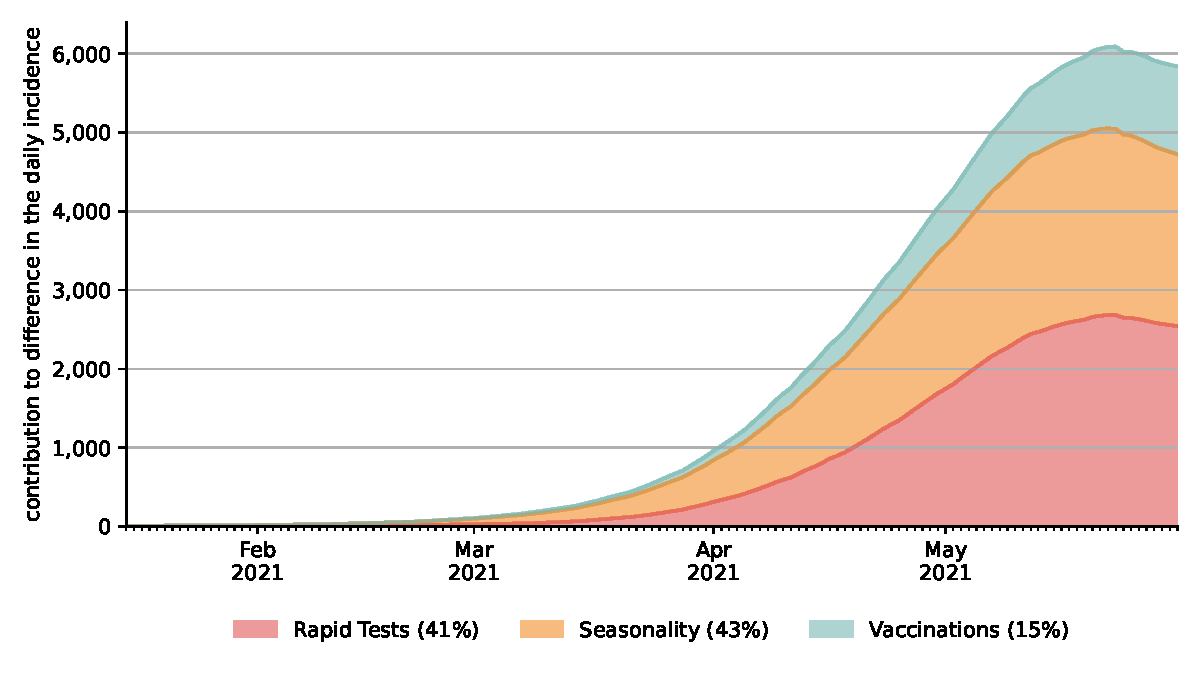
\includegraphics[width=0.9\textwidth]{figures/results/figures/data/testing/full_decomposition_channels_area_average}
            \caption{Shapley decomposition with average of sensitivity estimates}
        \end{subfigure}
        \begin{subfigure}[b]{0.475\textwidth}
            \centering
            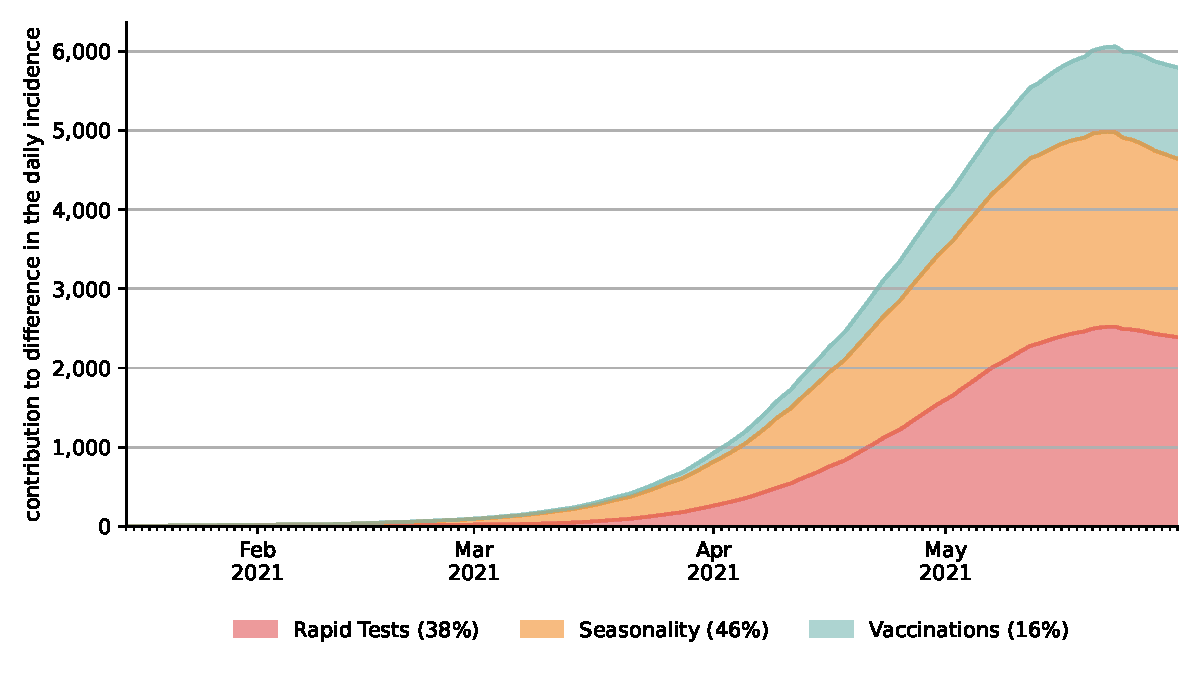
\includegraphics[width=0.9\textwidth]{figures/results/figures/data/testing/full_decomposition_channels_area_lower_envelope}
            \caption{Shapley decomposition with lower envelope of sensitivity estimates}
        \end{subfigure}

        \caption{Shapley decompositions for different values of rapid test sensitivity}
        \floatfoot{\noindent \textit{Note:} The figure shows updated versions of the
            Shapley decomposition in figure \ref{fig:2021_scenarios_decomposition}. The
            decompositions are based on 20 model runs with different random seeds. The
            share attributed to each channel is rounded to the next full percentage
            point to acknowledge the remaining sampling uncertainty.}
        \label{fig:robustness_to_sensitivity_assumptions}
    \end{figure}

    \FloatBarrier
}


\subsection{Share of Detected Cases}
\label{subsec:data_share_known_cases}

One important feature of our model is that we distinguish between undetected and detected
cases and that we model which cases are detected and which are not (see
Section~\ref{sub:testing} for a detailed description for how we model both rapid and PCR
tests). For our model it is important to have an estimate for the share of cases that is
detected in the absence of rapid tests ($\psi_t$). For this we rely on the
\cite[Dunkelzifferradar Project][]{Dunkelzifferradar2020} which uses estimates of the
case fatality rate to estimate the number of total cases given the number of CoViD-19
deaths which are assumed to be perfectly observable. For 2020, we follow the reported
share of detected cases quite closely. One exception is the phase of November 2020 where
we interpolate to maintain monotonicity during the fall as there was no reason why the
share of detected cases should have risen in that time\footnote{The testing policy
changed in November \citep{RKI2020a}. However, this only moved the rare PCR tests more
towards vulnerable groups.}

% After Christmas 2020
Since vaccinations started after Christmas 2020 and these were predominantly given to
nursing homes in the beginning and other vulnerable groups in spring, we expect the
relationship between deaths and the number of total infections to change rapidly in 2021.
This is why we stop using the share of detected cases estimated by the Dunkelzifferradar
after Christmas. Instead, we assume that the share of detected cases would have stayed
the same in the absence of rapid tests. Thus, we also achieve in our model an increase in
the share of detected cases but this is driven from inside our model through increased
rapid testing which lead follow-up PCR tests when they are positive (see
Section~\ref{subsec:results_share_known_cases} and \ref{sub:testing}).

% Christmas and Easter
Lastly, we model reductions in the share of detected cases due to the two major holidays in our
simulation period, Christmas and Easter. During both holidays many laboratories did not
process tests and most physicians' offices were closed, leading to less PCR tests and
short and large drops in the share of known cases. The resulting share of detected cases
in the absence of rapid tests is shown in Figure~\ref{fig:share_known_cases_data} and
was estimated to fit the data.

\begin{figure}[ht]
  \centering
  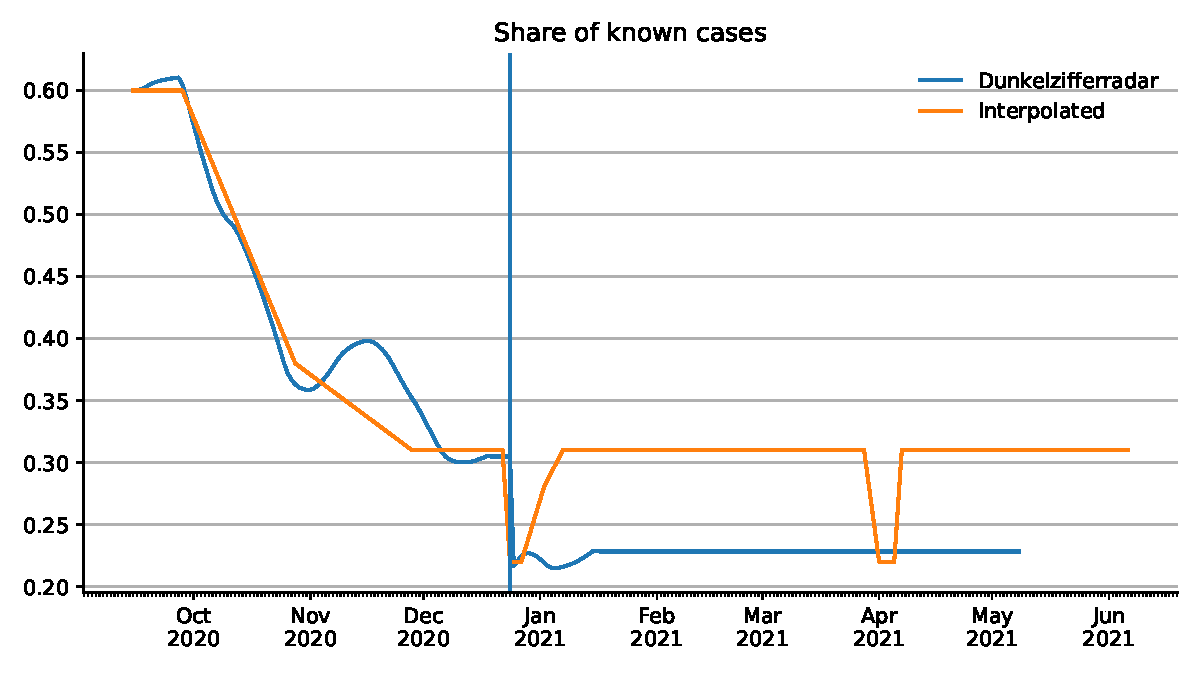
\includegraphics[width=0.5\textwidth]{figures/results/figures/data/testing/assumed_overall_share_known_cases}
  \caption{Share of Detected Cases in the Absence of Rapid Tests}
  \label{fig:share_known_cases_data}
  \floatfoot{\noindent \textit{Note:} The figure shows the share of cases that is
  reported as an official case via PCR confirmation. We use the overall share of known
  cases that was estimated through the case fatality ratio by the \cite[Dunkelzifferradar
  Project][]{Dunkelzifferradar2020} for all of 2020 and then assume it to be constant as
  vaccinations of the elderly strongly affect the case fatality rate which the project
  does not account for. Starting in 2021 in addition to the overall numbers of detected
  cases through symptoms and a random component, cases are also detected through
  confirmation of positive rapid tests which happens endogenously inside the model. For
  the public holidays of Christmas and Easter we lower the share of detected cases as
  fewer PCR tests are available during public holidays. See
  Figure~\ref{fig:share_known_cases_by_age_group} for how the share of detected cases
  develops in our model for each age group}.
\end{figure}

\FloatBarrier


\subsection{Simulated Rapid Tests}
\label{subsec:results_rapid_test_statistics}

In order to make most use out of limited data sources on rapid test usage, we model the
number of performed rapid tests as a result of time invariant willingness to do rapid
tests and time varying supply side factors and events that trigger rapid tests. Thus,
the parameters described in Section~\ref{subsec:rapid_test_demand} are only indirectly
related to the number of rapid tests that are actually performed in the model. When it
comes to positive and negative rapid tests, there is even an additional layer because
rapid tests imperfectly sensitive and specific.

In this section we look at how rapid tests expanded in our simulations over time and to
what degree they are useful as a screening device despite their imperfections.

We start with the share of the population doing a rapid test, receiving a positive rapid
test and receiving a negative rapid test over time by the channel through which the test
was demanded in Figures~\ref{fig:rapid_test_demand_by_channel},
\ref{fig:pos_rapid_tests_by_channel} and \ref{fig:neg_rapid_tests_by_channel},
respectively. Overall, the share of the population getting a rapid test on a given day
increases from 2\% in mid March to over 10\% by May. The work rapid tests are a little
ragged because of public holidays. For education rapid tests both vacations (first half
of April) as well as the opening of schools in May are very visible in the rapid test
demand. Overall, work tests make up the largest fraction of rapid tests. The image is
very similar for the share of positive tests, except that the overall number of positive
tests starts decreasing in May as rapid test expansion comes to a halt and cases fall,
especially the positive share of private rapid tests falls as less and less individuals
are triggered to seek a rapid test because of a risk contact in their household.

\begin{figure}[ht] % Share tested per day
  \centering
  \begin{subfigure}[b]{0.3\textwidth}
      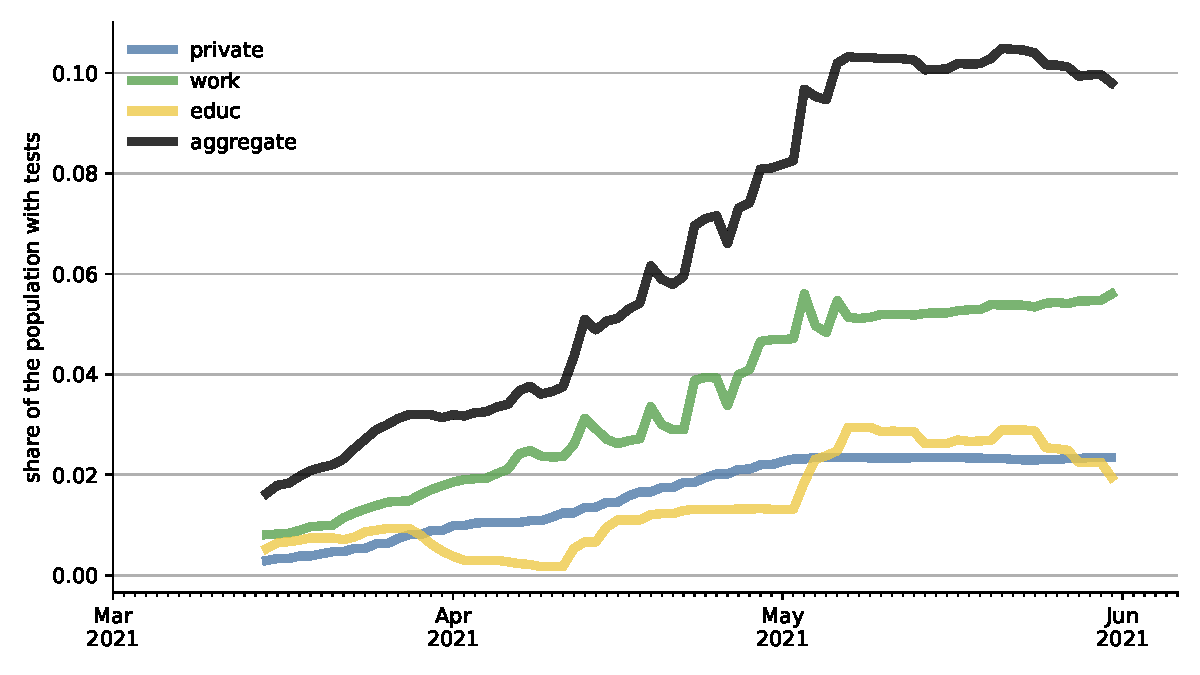
\includegraphics[width=\textwidth]{figures/results/figures/rapid_test_statistics/popshare_tested}
      \caption{Share of the Population Doing a Rapid Test Because of Different Channels
      on a Given Day}
      \label{fig:rapid_test_demand_by_channel}
  \end{subfigure}
  \hfill
  \begin{subfigure}[b]{0.3\textwidth}
      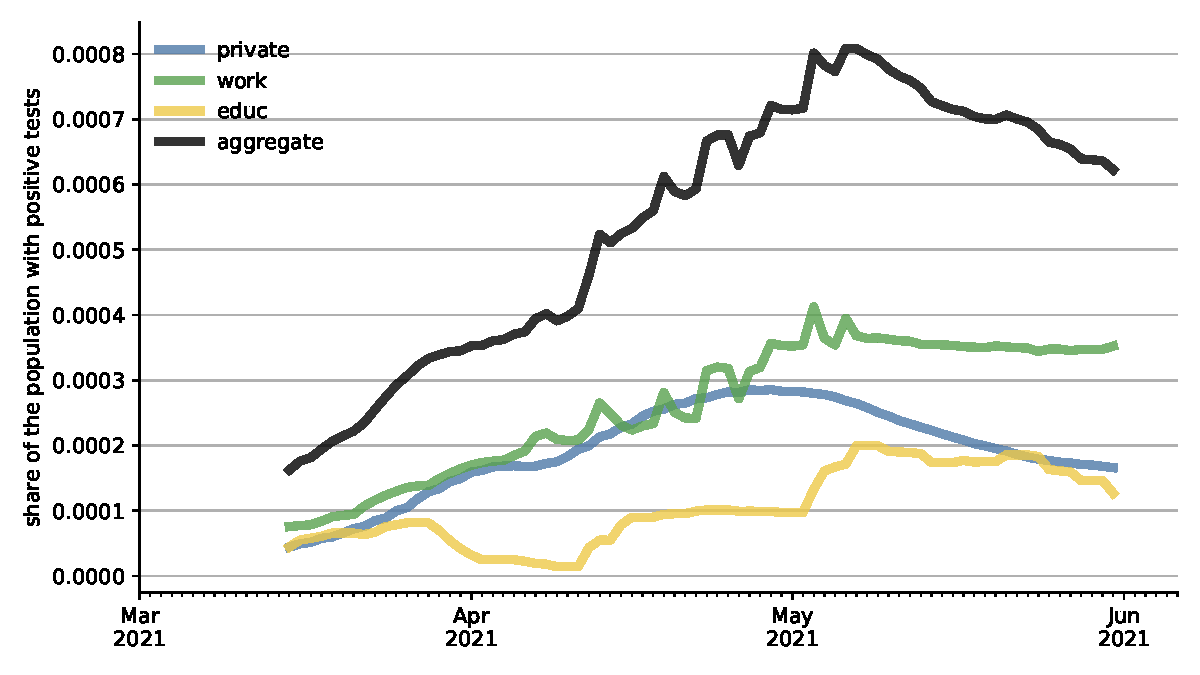
\includegraphics[width=\textwidth]{figures/results/figures/rapid_test_statistics/popshare_tested_positive}
      \caption{Share of the Population Testing Positive Because of Different Channels
      on a Given Day}
      \label{fig:pos_rapid_tests_by_channel}
  \end{subfigure}
  \hfill
  \begin{subfigure}[b]{0.3\textwidth}
      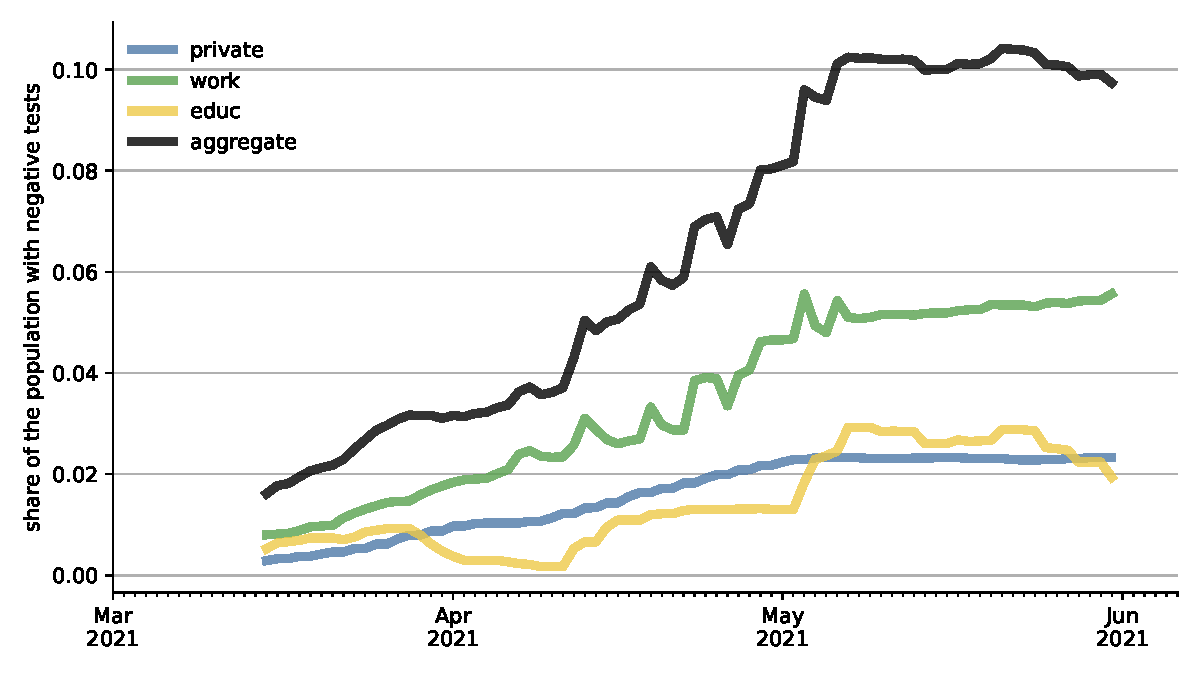
\includegraphics[width=\textwidth]{figures/results/figures/rapid_test_statistics/popshare_tested_negative}
      \caption{Share of the Population Testing Negative Because of Different Channels
      on a Given Day}
      \label{fig:neg_rapid_tests_by_channel}
  \end{subfigure}
  \caption{Rapid Test Shares in the Population by Channel}
  \floatfoot{\noindent \textit{Note:}
    Rapid tests in the education setting are demanded by teachers (nursery, preschool and
    school) as well as pupils. After Easter the required frequency of tests is
    increased from once per week to twice per week. Work rapid tests are demanded by
    individuals that still have work contacts, i.e. do not work from home. The share of
    employers offering rapid tests increases over the time frame and the frequency of
    testing is also increased. Private tests are demanded by individuals for one of three
    reasons: having developed symptoms without access to a PCR test, having a household
    member that has tested positive or developed symptoms or having planned a weekly
    meeting with friends. The left figure shows the share of the population doing a
    rapid test on a given day. The middle figure shows the share of the population
    testing positive on a given day (true and false positives). The right figure shows
    the share of the population testing negative on a given day (true and false
    negatives).}
\end{figure}

\FloatBarrier

Next, we show the tests split by whether they are true positive, false positive, true
negative or false negative (see Figure~\ref{fig:rapid_test_results_numbers}) in numbers
per million individuals to make the metric comparable to incidences.
% true positive
The number of true positives (Figure~\ref{fig:rapid_tests_number_true_positive}) rapidly
increases and peaks at the end of April with over 200 cases per million detected through
rapid tests per day. This means that our model suggests that Germany was able to detect
up to 16,600 cases per day that would have likely gone undetected otherwise. The most
powerful tool for detecting cases are the private rapid tests. This is because a large
share of them are targeted, i.e. triggered by events in the household. However, this
does not mean that rapid tests in the workplace or at school are useless. It is rather
the combination of large scale screening at work and in schools and very efficient
follow up tests whenever those screening tests detected a case. Shapley values
(Figure~\ref{fig:2021_scenarios_decomposition_tests}) take this into account and
assign about 50\% of the overall reduction of case numbers via rapid tests to private
rapid tests with work and school rapid tests accounting for 40\% and 7\%,
respectively.

Such a large effect of rapid tests seems to be at odds with the general perception that
they are not very reliable. However, this is not the case, which can be seen from the
number of
false negative tests. At its peak at the beginning of May, there are more than 80 false
negative rapid tests per million inhabitants per day. While this number might sound low
in isolation, it becomes quite large when set in context: We estimate that at at the
the same time only 200 cases per million are detected by rapid tests. This means that
even at the time where discovery of cases via rapid tests is at its peak, almost
30\% of of people who are infected and make a test are not discovered by the test.

This shows clearly that the large effect of rapid tests on the infection dynamic
is not driven by unrealistic assumptions about their sensitivity but rather by the
fact that there was a very large number of infected individuals who did not know they
are positive. Detecting and isolating some of them is enough to slow down the
overall infection dynamic.

\begin{figure}   % Number of True Positive / False Positive / True Negative / False Negative
    \centering
    \begin{subfigure}[b]{0.425\textwidth}
        \centering
        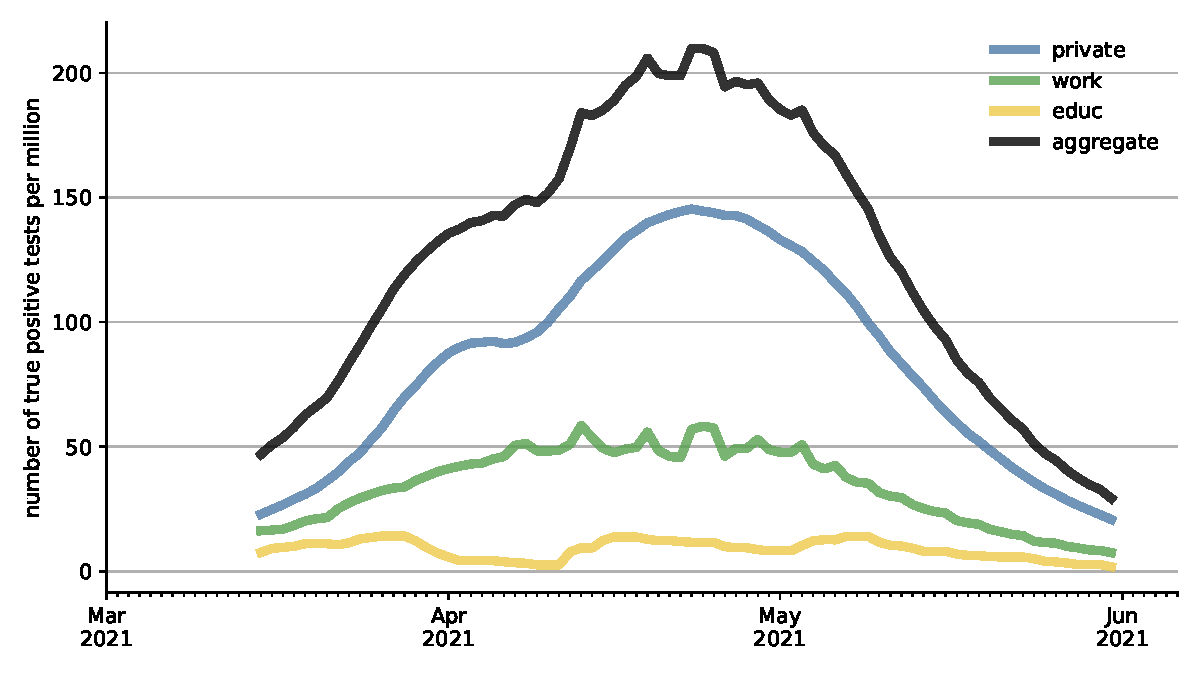
\includegraphics[width=\textwidth]{figures/results/figures/rapid_test_statistics/number_true_positive}
        \caption{Number of Discovered Cases Due to Rapid Tests by Channel}
        \label{fig:rapid_tests_number_true_positive}
    \end{subfigure}
    \hfill
    \begin{subfigure}[b]{0.425\textwidth}
        \centering
        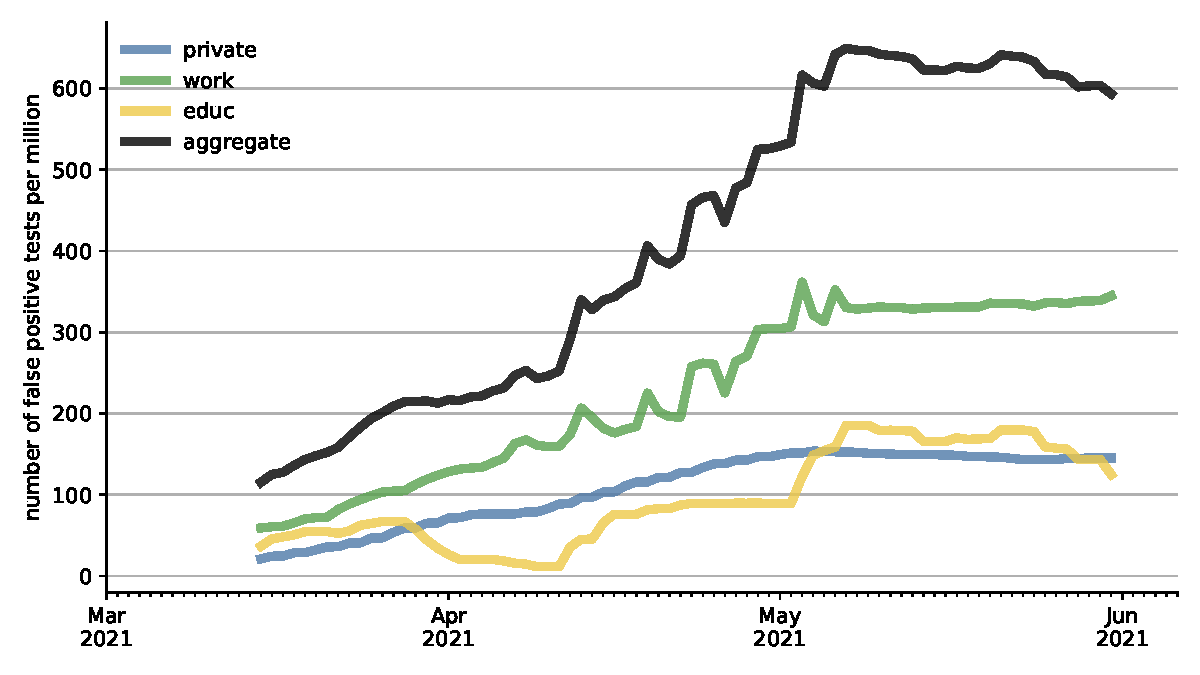
\includegraphics[width=\textwidth]{figures/results/figures/rapid_test_statistics/number_false_positive}
        \caption{Number of False Positive Rapid Tests by Channel}
        \label{fig:rapid_tests_number_false_positive}
    \end{subfigure}
    \vskip3ex
    \begin{subfigure}[b]{0.425\textwidth}
        \centering
        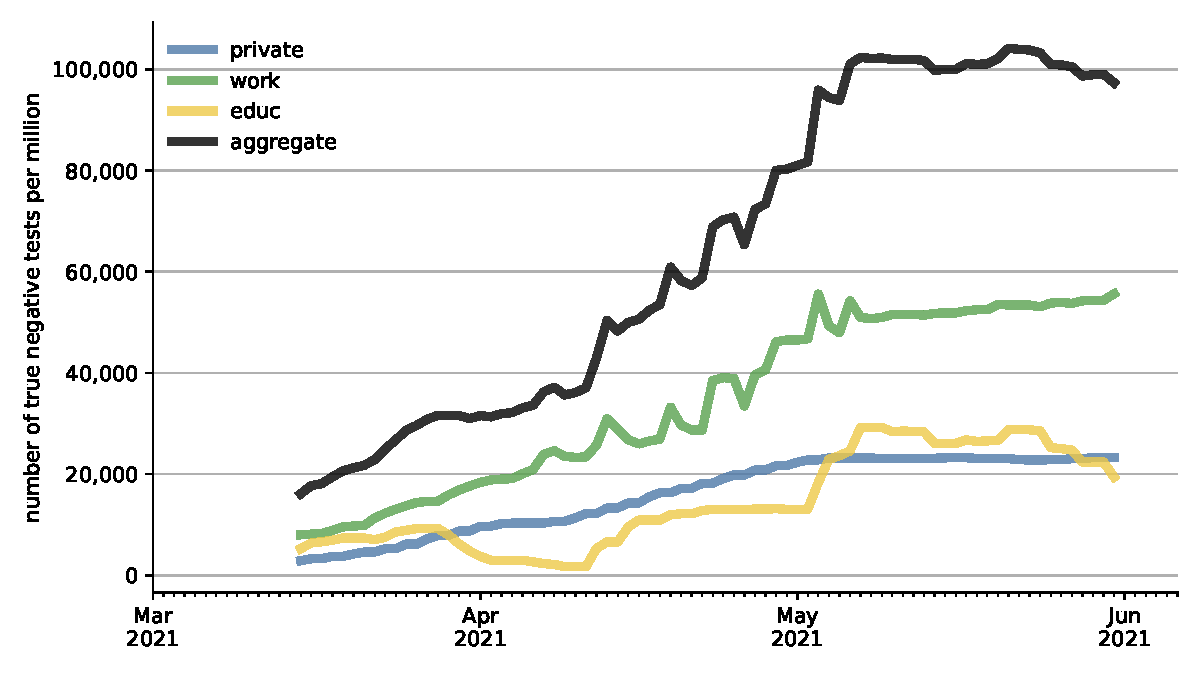
\includegraphics[width=\textwidth]{figures/results/figures/rapid_test_statistics/number_true_negative}
        \caption{Number of True Negative Rapid Tests by Channel}
        \label{fig:rapid_tests_number_true_negative}
    \end{subfigure}
    \hfill
    \begin{subfigure}[b]{0.425\textwidth}
        \centering
        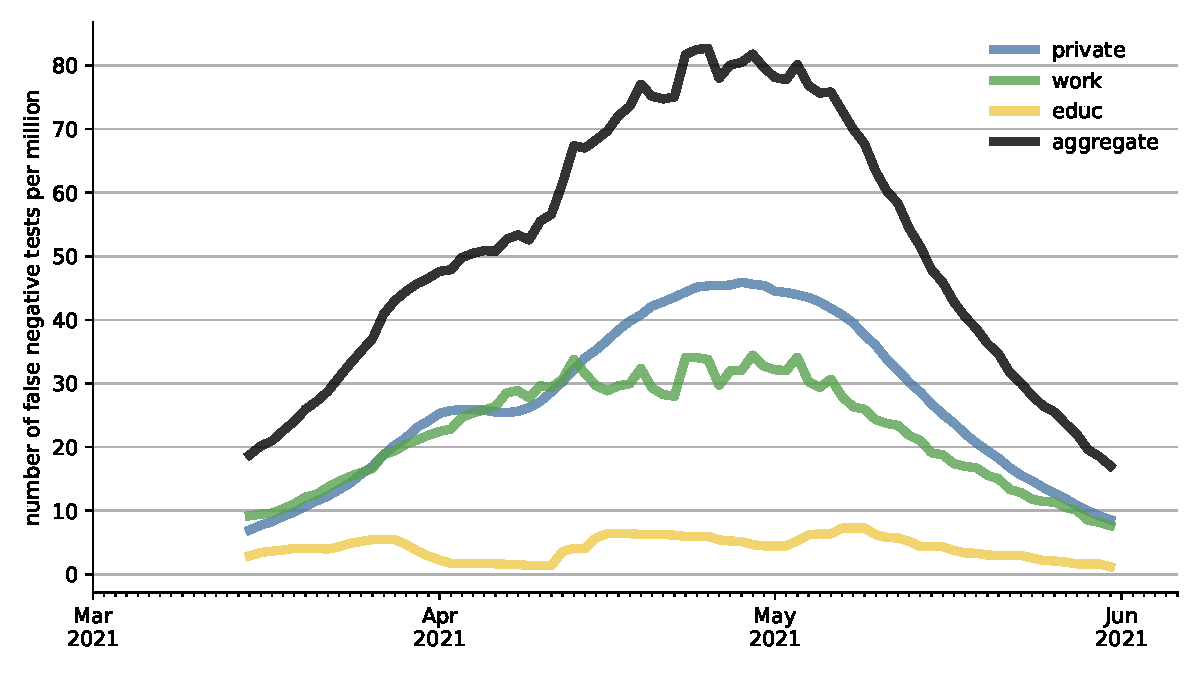
\includegraphics[width=\textwidth]{figures/results/figures/rapid_test_statistics/number_false_negative}
        \caption{Number of False Negative Rapid Tests by Channel}
        \label{fig:rapid_tests_number_false_negative}
    \end{subfigure}
    \vskip3ex
    \caption{Rapid Test Results}
    \label{fig:rapid_test_results_numbers}
    \floatfoot{\noindent \textit{Note:}
    Each panel shows the number of rapid tests per million inhabitants that fall into the
    respective category. Private rapid tests are especially good at detecting cases but
    since they are often triggered by rapid tests from other channels, the other groups
    of tests, especially rapid tests at the workplace, also play an important role for
    containing the pandemic.}
\end{figure}

\FloatBarrier

A similar picture arises, when looking at the false positive rate,
i.e. the share of positive tests that go to people who are not infected.
Figure~\ref{fig:rapid_tests_false_positive_rate} shows that the false
positive rate is very high. On average 60\% to 93\% of positive tests are
received by individuals that are not infected. The false positive rate increases over
time. This is due to the low prevalence of infections in the population, which falls
over time. Again, private rapid tests are an exception with a much lower false
positive rate because those tests are primarily demanded when there is a high likelihood
of being infected. The low false negative rate of 0.2\% looks very low. As discussed
above this is deceiving and just a mechanical consequence of a very low prevalence
of the disease and the many rapid tests done by non-infected people.

\begin{figure} % True Positive / False Positive / True Negative / False Negative Rate
    \centering
    % \begin{subfigure}[b]{0.425\textwidth}
    %     \centering
    %     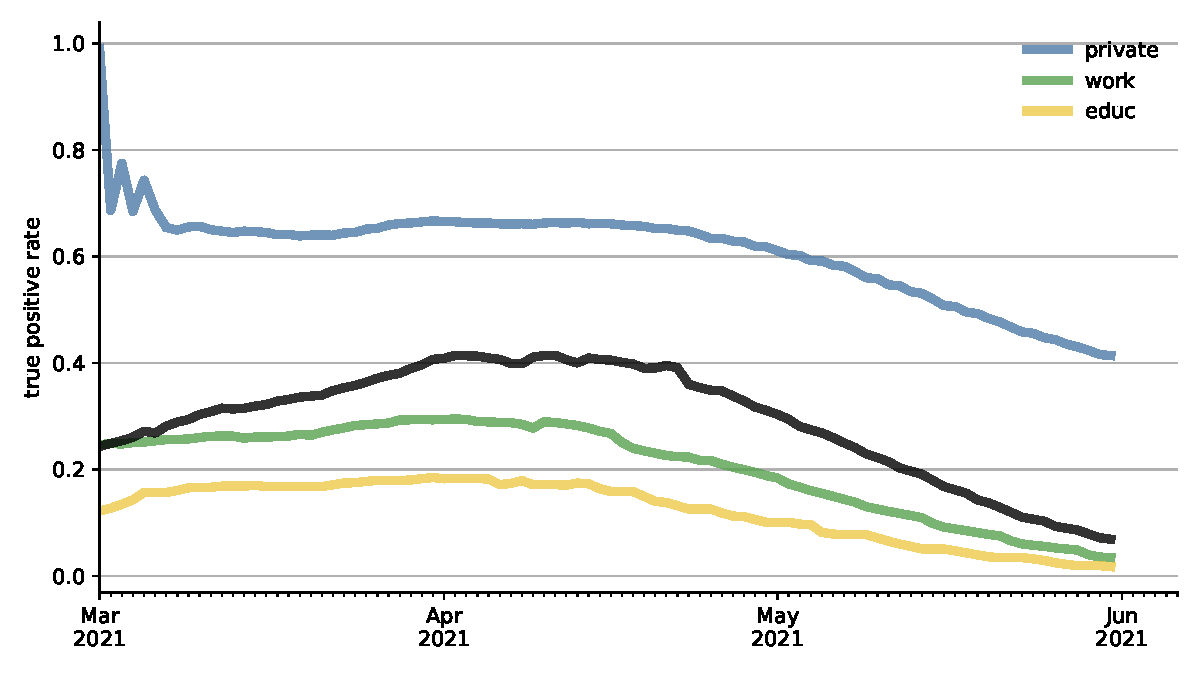
\includegraphics[width=\textwidth]{figures/results/figures/rapid_test_statistics/true_positive_rate}
    %     \caption{Rate of True Positive Rapid Tests by Channel}
    %     \label{fig:rapid_tests_true_positive_rate}
    % \end{subfigure}
    % \hfill
    \begin{subfigure}[b]{0.425\textwidth}
        \centering
        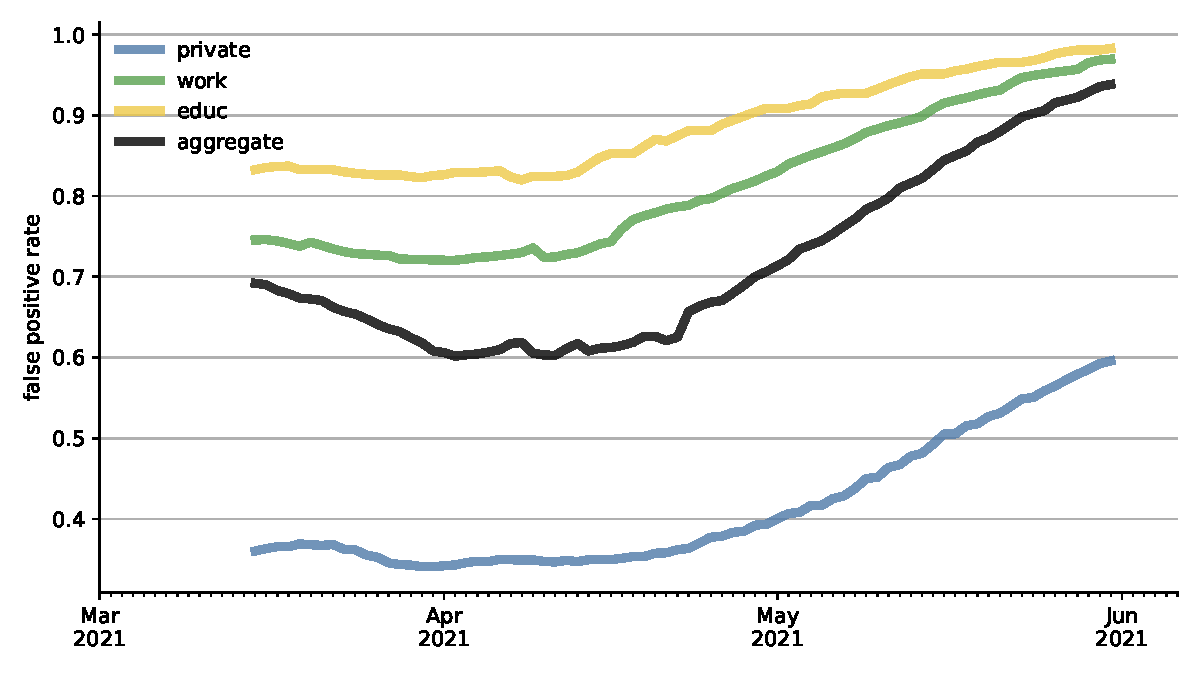
\includegraphics[width=\textwidth]{figures/results/figures/rapid_test_statistics/false_positive_rate}
        \caption{Rate of False Positive Rapid Tests by Channel}
        \label{fig:rapid_tests_false_positive_rate}
    \end{subfigure}
    % \vskip3ex
    % \begin{subfigure}[b]{0.425\textwidth}
    %     \centering
    %     \includegraphics[width=\textwidth]{figures/results/figures/rapid_test_statistics/true_negative_rate}
    %     \caption{Rate of True Negative Rapid Tests by Channel}
    %     \label{fig:rapid_tests_true_negative_rate}
    % \end{subfigure}
    \hfill
    \begin{subfigure}[b]{0.425\textwidth}
        \centering
        \includegraphics[width=\textwidth]{figures/results/figures/rapid_test_statistics/false_negative_rate}
        \caption{Rate of False Negative Rapid Tests by Channel}
        \label{fig:rapid_tests_false_negative_rate}
    \end{subfigure}
    \vskip3ex
    \caption{Rapid Test Rates by Channel}
    \label{fig:rapid_test_results_rates}

    \floatfoot{\noindent \textit{Note:}
    The left panel shows the share of positive tests that are given to people who are not
    infected. This share is large as can be expected with a very low baseline rate of
    positive individuals. As the incidence in the population drops, the false positive
    rate increases. An exception are the private rapid tests because they are --
    especially when the incidence is high -- often triggered by events that make it
    likely that the test taker is infected and therefore their false positive rate is
    much lower. The right panel shows the false negative rate in the population, i.e. the
    share of negative test results that are mistakenly given to infected individuals.
    This is very low because there are many truly negative tests in times of low
    incidences and large scale screening tests.}
\end{figure}

\FloatBarrier




\subsection{Scenarios} \comment[id=K]{Add parameter notation when writing this.}
\label{subsec:appendix_scenarios}


\begin{figure}[ht] % Work Scenarios
  \centering
  \begin{subfigure}[b]{.49\textwidth}
    \centering
    \includegraphics[width=0.9 \textwidth]{figures/results/figures/scenario_comparisons/new_work_scenarios/full_new_known_case}
    \caption{Reported Cases}
    \label{fig:work_scenarios_new_known_case}
  \end{subfigure}
  \hfill
  \begin{subfigure}[b]{.49\textwidth}
    \centering
    \includegraphics[width=0.9 \textwidth]{figures/results/figures/scenario_comparisons/new_work_scenarios/full_newly_infected}
    \caption{Total Cases}
    \label{fig:work_scenarios_newly_infected}
  \end{subfigure}
  \caption{The Effect of Different Work Scenarios on Reported and Total Cases}
  \label{fig:work_scenarios_detailed}
  \floatfoot{\noindent \textit{Note:} The figure shows the development of cases after the
  policy changes took place at Easter until the end of our simulation period (end of
  May). We vary the share of workers that work from home and how many tests are performed
  at work relative to our baseline scenario. Making it mandatory to test all employees
  that do not work from home markedly reduces cases -- even when only assuming 95\%
  compliance on both the employer and the employee side. As before, the observed cases
  can be misleading because more testing leads to more detected cases. It takes two to
  three weeks for the reduction in new infections effect to dominate the increased
  detection effect. Furthermore, the two opposing effects lead to a smaller effect size
  than is actually the case.}
\end{figure}

 \comment[id=K]{Regarding figure \ref{fig:work_scenarios_detailed}: Look up numbers and
 add them to the description.}


\begin{figure}[ht] % School Scenarios
  \centering
  \begin{subfigure}[b]{.49\textwidth}
    \centering
    \includegraphics[width=0.9 \textwidth]{figures/results/figures/scenario_comparisons/school_scenarios/full_new_known_case}
    \caption{Reported Cases}
    \label{fig:school_scenarios_new_known_case}
  \end{subfigure}%
  \hfill
  \begin{subfigure}[b]{.49\textwidth}
    \centering
    \includegraphics[width=0.9 \textwidth]{figures/results/figures/scenario_comparisons/school_scenarios/full_newly_infected}
    \caption{Total Cases}
    \label{fig:school_scenarios_newly_infected}
  \end{subfigure}
  \caption{The Effect of Different School Scenarios on Reported and Total Cases}
  \label{fig:school_scenarios_detailed}
  \floatfoot{\noindent \textit{Note:} The figure shows the development of cases after the
   policy changes took place at Easter until the end of our simulation period (end of
   May). Apart from the enacted school policies as our baseline we simulate how cases
   would have developed if schools had been closed completely as the strictest possible
   counterfactual scenario and two opening models: One where schools open normally (with
   hygiene measures) without any testing in the education sector and one where schools
   open normally but testing shares develop as in the baseline scenario. Our simulations
   suggest that the enacted policies were as effective as keeping schools closed. Opening
   schools with the testing schemes that were in place after Easter would have had a
   small effect on the overall incidence. However, this is mainly due to the stringent
   testing that was in place in schools by that time. Had schools opened without testing
   requirements the total incidence would have been up to 50 points higher, though this
   would have been less visible in the reported cases.}
\end{figure}

 \comment[id=K]{Regarding figure \ref{fig:school_scenarios_detailed}: Look up numbers and
 add them to the description.}


\begin{figure}[ht] % Random Rapid Tests
  \centering
  \begin{subfigure}[b]{.49\textwidth}
    \centering
    \includegraphics[width=0.9 \textwidth]{figures/results/figures/scenario_comparisons/random_rapid_tests_vs_baseline/full_new_known_case}
    \caption{Reported Cases}
    \label{fig:random_rapid_tests_new_known_case}
  \end{subfigure}%
  \hfill
  \begin{subfigure}[b]{.49\textwidth}
    \centering
    \includegraphics[width=0.9 \textwidth]{figures/results/figures/scenario_comparisons/random_rapid_tests_vs_baseline/full_newly_infected}
    \caption{Total Cases}
    \label{fig:random_rapid_tests_newly_infected}
  \end{subfigure}
  \caption{The Role of Targeted and Compliance Driven Rapid Test Demand}
  \label{fig:random_rapid_tests_detailed}
  \floatfoot{\noindent \textit{Note:} \textcolor{red}{To be written}}
\end{figure}

 \comment[id=K]{Describe that random tests are more effective at detecting cases and that
 explains the bump in the random test scenario detection in the beginning. However, cases
 fall immediately more in the non-random scenario because the targeted demand for tests
 by household members leads to a much more efficient interruption of infection chains
 because we catch the household members very early in their infectious period.}

 \comment[id=K]{Write that at the end of our simulation period nearly everyone in the
 educ sector did rapid tests because they are mandatory but still 40-50\% refusers in the
 work and private sector}

\FloatBarrier




        \begin{refcontext}[sorting=none]
            \printbibliography[heading=bibintoc]
        \end{refcontext}

    \end{refsection}

\end{appendices}

\end{document}
